\chapter[Spracheinstellungen und Sprachideologien]{Spracheinstellungen und Sprachideologien als Einflussfaktoren für Sprachvariation und -wandel}
\label{cha:SprachideologienundSpracheinstellungen}
Im folgenden Kapitel geht es um zentrale Konzepte, die für die Frage relevant sind, wie die Vorstellungen von Sprachbenutzer:innen über Sprache untersucht werden können und wie sie die Variation und den Wandel von Sprachgebrauch beeinflussen. 
\autoref{sec:MetapragmatikinderLinguistik} thematisiert zunächst die Relevanz der Beschäftigung mit der {Re\-flexion} über Sprache und mit den Sprachgebrauch bewertenden, metapragmatischen Äußerungen in der Linguistik. 
In \autoref{sec: Forschungsansaetze} werden die zwei wesentlichen Ansätze vorgestellt, die sich hier abseits normativer Perspektivierungen\footnote{Mit normativ ausgerichteten Perspektiven auf Sprache beschäftigt sich die linguistische Sprachkritik, die hier nicht thematisiert werden soll \citep[s. bspw.][]{Kilian2010}.} herausgebildet haben, die Spracheinstellungsforschung und die Sprachideologieforschung. 
Anschließend geht es in \autoref{sec:MetapragmatikVariationWandel} um die Interdependenz zwischen Sprachurteilen, Variation und Wandel im Sprachgebrauch. 

\section{Reflexion über Sprache als zentraler Gegenstand der Linguistik}
\label{sec:MetapragmatikinderLinguistik}
\largerpage

Das Interesse daran, wie Sprache konzeptualisiert wird und wie dies mit dem Sprachgebrauch und dem Wandel sprachlicher Strukturen zusammenhängt, ist seit dem Ende des letzten Jahrhunderts in der Linguistik deutlich gestiegen (\cites[s. etwa][5--6]{Jaworski.2004}[119]{Garrett.2007}). 
Im Folgenden geht es zunächst darum, was metapragmatische Äußerungen sind und inwiefern und warum sie für die Linguistik einen interessanten und relevanten Untersuchungsgegenstand darstellen (\autoref{sec:MetapragmatischeAeusserungen}). 
Dabei wird hier mit Metapragmatik bewusst ein Begriff verwendet, den die Sprachideologieforschung geprägt hat, während in der Spracheinstellungsforschung häufig bspw. von Laienurteilen die Rede ist. 
\autoref{sec:Laienlinguistik} diskutiert den  Status metapragmatischer Äußerungen als \glqq Laienurteile\grqq. \autoref{sec:MetapragmatischeBewusstheit} beschäftigt sich mit der Frage, wieso über bestimmte sprachliche Phänomene bewusst reflektiert wird, während andere nicht thematisiert werden.
\subsection{Formen und Funktionen metapragmatischer Äußerungen}
\label{sec:MetapragmatischeAeusserungen}
Metapragmatische Äußerungen sind (sprachliche) Handlungen, die Werte und Einstellungen gegenüber Sprache, sprachlichen Formen oder sprachlichen Handlungen transportieren (\cites[s.][33]{Silverstein1993}[264]{Spitzmuller2013}[323--324]{Spitzmuller2014}). 
%Was ist Metapragmatik
Lässt sich Pragmatik beschreiben als {\glqq}how speech forms are used as effective action in specifiable cultural contexts{\grqq} \citep[3]{Silverstein.1981}, so zählen {\"A}u{\ss}erungen zu den Regelhaftigkeiten solchen Gebrauchs zur Metapragmatik:~{\glqq}To give those rules, to talk about them, is to engage in {\glq}metapragmatic{\grq} discourse, we should say{\grqq}~\citep[3--4]{Silverstein.1981}.\footnote{Das ebenfalls verwandte Konzept der Sprachkritik kann als eine Form von Metapragmatik gewertet werden \citep[s.][3]{Schiewe.2005}.} 
Damit ist Metapragmatik immer reflexiv: Sprachliches Handeln wird genutzt, um über sprachliches Handeln zu sprechen~\citep[s.][116]{Gal.2016}. 

Mit dem Konzept der Metapragmatik eng verwandt ist das Konzept der Metasprache, das bereits von \citet[]{Jakobson.1960} als eine zentrale Funktion von Sprache beschrieben wird. 
Im Vergleich zur Metasprache  geht es bei der Metapragmatik nicht ausschließlich um sprachliche Äußerungen über Sprache, sondern um jedes Verhalten, das Sprachgebrauch und das Handeln mit Sprache bewertet.
Die Metapragmatik ist damit kein Randbereich, sondern eine zentrale Funktion von Sprache und somit auch ein zentrales Interessensgebiet der Linguistik (\cites[s.][1--2]{Cameron1995}[3]{Jaworski.2004}[113]{Gal.2016}). 
%Formen metapragmatischer Äußerungen
Die Relevanz dieses Bereichs zeigt sich unter anderem an der Beobachtung, dass alle Sprachgemeinschaften Sprache nutzen, um über Sprache zu sprechen: 
\begin{quote}Several genres of metapragmatic discourse occur naturally in all language communities---e.g., verbal reports and glosses of language use; names for registers and associated speech genres; stereotypes about users of a repertoire; proscriptions on usage; standards of appropriate usage; positive or negative assessments of the social worth of the register.~\citep[][217]{Agha.1999}\end{quote}
Metapragmatische Äußerungen bilden Diskurse über Sprache, zu denen etwa sprachpflegerische Schriften wie die Bastian Sicks, journalistische Texte über Sprache und ihren Gebrauch, linguistische Aufsätze, Vorträge, Schulbücher sowie der Schulunterricht, Ratgeber, aber auch private Unterhaltungen und einzelne Kommentare zu Sprachgebräuchen zählen (zum Begriff des Diskurses s. \citealp{Foucault.1974}). 
Metapragmatische Äußerungen, die Teil solcher Diskurse sind, können dabei unterschiedlicher Natur sein. 
Typische Beispiele wären etwa \object{in Norddeutschland sagt man Moin} oder \object{kennenzulernen schreibt man zusammen}. 
\citeauthor{Agha2007} macht aber darauf aufmerksam, dass metasprachliche Handlungen nicht nur verbale {\"A}u{\ss}erungen sein k{\"o}nnen:~{\glqq}An eyebrow raised in response to a remark implicitly evaluates the import of that remark and is, to this extent, a metalinguistic act{\grqq}~\citep[17]{Agha2007}. 
Auch \citet[21]{Konig.2017} betont die Relevanz nonverbaler Bewertungssignale. 
Im Bereich des massenmedial vermittelten Diskurses ist etwa an die Bebilderung von Zeitungs- und Zeitschriftenartikeln zu denken \citep[s.][]{Spitzmuller.2007}. 

Nicht nur explizit wertende Äußerungen oder Handlungen fallen in den Bereich der Metapragmatik, sondern auch Aussagen, die sprachliche Handlungen kategorisieren oder beschreiben.\footnote{\citet[]{Silverstein.2018} nennt außerdem implizite Formen der Metapragmatik. Hierzu zählt er bestimmte Formen der Intertextualität, Voicing und Metrikalisierung. Da diese Formen der Metapragmatik für die Analyse in der vorliegenden Studie nicht relevant sind, wird auf sie hier nicht eingegangen.}
Teilweise wird bei Metasprache oder Metapragmatik zwischen verschiedenen Komponenten unterschieden:~Unter Metasprache1 werden dann explizite, oft wertende Aussagen verstanden, während mit Metasprache2 bspw. Sprechhandlungsbezeichnungen wie \object{sagen} gemeint sind, mit Metasprache3 hingegen keine expliziten {\"A}u{\ss}erungen, sondern die diesen zugrundeliegenden kognitiven Strukturen, die sonst meist unter Sprachbewusstheit gefasst werden (\citealp[s.][16--19]{Cuonz.2014} sowie \autoref{sec:MetapragmatischeBewusstheit}). 
Besser als diese Typologie scheint jedoch das Konzept der metapragmatischen Transparenz von \citet[16--17]{Silverstein.1981} geeignet, das danach fragt, wie nah eine metapragmatische Beschreibung an der objektsprachlichen {\"A}u{\ss}erung ist: \object{Sie hat versprochen, einzukaufen} als Beschreibung von \object{Ich verspreche, einzukaufen} hat etwa eine hohe metapragmatische Tranzparenz~\citep[s.][16--17]{Silverstein.1981}.

Neben Äußerungen, die sprachliche Formen bewerten und einordnen, zählen zu den metapragmatischen Äußerungen auch Aussagen über den eigenen Sprachgebrauch wie etwa \object{Ich verwende Großschreibung in E-Mails}. 
\citet[50]{Cavanaugh.2013} betont, dass von solchen metapragmatischen {\"A}u{\ss}erungen einer Person nicht auf ihren tats{\"a}chlichen Umgang mit sprachlichen Formen geschlossen werden kann (s. dazu auch \citealp[43]{Silverstein.1976} sowie \autoref{sec:Komponenten}). 

Sprecher:innen berufen sich bei metapragmatischen {\"A}u{\ss}erungen auf in der Gesellschaft geteilte, nicht hinterfragte Annahmen über Sprache (s. \cites[1]{Gunthner.2012}[205]{Konig2015}). 
Die Metapragmatik ist also immer auf der einen Seite von tradierten Vorstellungen über Sprache, den Sprachideologien, geprägt, auf der anderen Seite bringt sie persönliche Einstellungen gegenüber Sprache zum Ausdruck (\cites[s.][196--197]{Silverstein2003}[1319]{Vandermeeren2005}{Spitzmuller2013}; \autoref{sec:Integrationsversuch}). 
Gleichzeitig lässt sich Metapragmatik als diskursive Aushandlung von Wissen und Meinungen über Sprache fassen \citep[s.][263]{Spitzmuller2013}. 
Für die Beschäftigung mit metapragmatischen Diskursen ist es daher sehr wichtig, ihre Einbettung in Traditionen der jeweiligen Zeit zu berücksichtigen, d.\,h., sowohl synchron als auch diachron zu arbeiten \citep[s.][325]{Spitzmuller2014}. 
Bspw. wird in der {\"o}ffentlichen Sprachkritik als Ma{\ss}stab h{\"a}ufig die Kommunikationsf{\"a}higkeit als entscheidendes Kriterium angef{\"u}hrt und so die denotative Funktion sprachlicher Zeichen, also ihre Darstellungsfunktion -- scheinbar -- in den Vordergrund ger{\"u}ckt (\cites[s.][]{Buhler.1999}[190]{Spitzmuller.2007}[322]{Langer.}[128]{Silverstein.2014}). 
Damit wird an einen verbreiteten Sprachmythos angeknüpft, der bereits in Platons Kratylos-Dialog existiert (\cites[s.][57]{Heringer.2015}[116]{Gal.2016}). 
Mit der Darstellungsfunktion von Sprache hat die Kritik an bestimmten Formen allerdings meist nur vordergr{\"u}ndig zu tun, kritisiert wird vielmehr die Appellfunktion \citep[s.][]{Buhler.1999}. 
Tatsächlich zielt die Kritik also auf Werte ab, die mit dem kritisierten Sprachgebrauch verbunden sind. 
So teilen etwa diejenigen, die Anglizismen ablehnen, die Werte derer nicht, die Anglizismen verwenden und guthei{\ss}en~\citep[s.][191]{Spitzmuller.2007}.
Kritik an bestimmten Ausdrucksformen ist daher immer auch Kritik an den mit diesen assoziierten Gruppen~\citep[s.][191]{Spitzmuller.2007}. 

Metapragmatische Urteile haben zum einen eine komplexit{\"a}tsreduzierende Funktion, indem sie Zusammenh{\"a}nge in der Welt erkl{\"a}ren und vereinfachend darstellen. 
Zum anderen werden im metasprachlichen Diskurs soziale Normen ausgehandelt. 
Hier entscheidet sich etwa, in welcher Situation bestimmte Formen angemessen sind, welchen Gruppen ein bestimmter Sprachgebrauch zugewiesen wird und wie bestimmte Formen und damit auch Personen, die diese nutzen, wahrgenommen werden~(s. \cites[17]{Agha2007}[200]{Konig2015}). 
Diese Normen dienen zu einem wesentlichen Teil der sozialen Differenzierung und wirken gruppenkonstituierend bzw. gruppenfestigend, etwa indem Normabweichungen mit Ausgrenzung sanktioniert werden (\cites[s.][3]{Garrett2003}[33]{Garrett.2012}[114]{Gal.2016}).
Metapragmatische Diskurse haben damit eine hohe gesellschaftliche Relevanz.
Nach der Auffassung von \citet[103]{Arendt2015} ist es daher die Aufgabe der Linguistik, Sprachnormen nicht nur auf der Grundlage des beobachtbaren Sprachgebrauchs, sondern auch auf der Grundlage metasprachlicher {\"A}u{\ss}erungen von Sprachbenutzer:innen zu beschreiben.
 
\subsection{Laienlinguistische Sprachurteile}
\label{sec:Laienlinguistik}
Häufig werden Studien, die sich mit wertenden Urteilen über Sprache beschäftigen, in das Feld der Laienlinguistik eingeordnet (bzw. \textit{folk linguistics} im englischsprachigen Raum). 
Damit soll betont werden, dass Urteile von Sprecher:innen ohne wissenschaftlich-linguistische Ausbildung in den Blick genommen werden \citep[s.][25--26]{Antos1996}. 
Auf die Problematik der Bezeichnung wurde jedoch bereits vielfach hingewiesen (s. etwa \cites{Cuonz.2014}{Konig.2014}[396]{Moschonas2014}[320]{Spitzmuller2014}). 
Schwierig bis unmöglich ist bereits die Abgrenzung der Gruppe der Lai:innen. 
\citet[11--12]{Konig.2014} f{\"u}hrt verschiedene Definitionen f{\"u}r linguistische Lai:innen auf und h{\"a}lt fest, dass die Gruppe vor allem negativ als {\glqq}Nichtlinguisten{\grqq} definiert wird (etwa bei \citealp[179]{Garrett.2012}, aber auch bei \citealp[8]{Hennig2016}). 
Eine solche Definition ist aber nicht zielführend. 
So weist \citet{Konig.2014} darauf hin, dass sich Sprecher:innen nicht ohne Weiteres in eine Gruppe von Lai:innen und eine Gruppe von Expert:innen unterteilen lassen:
\begin{quote}Es kann daher nicht in allen F{\"a}llen allein aus der Tatsache, dass jemand keinen sprachwissenschaftlichen Studiengang belegt hat, auf ein linguistisches Nicht-Wissen in dem zu untersuchenden Bereich geschlossen werden;~umgekehrt kann aber auch nicht bei allen Linguist:innen automatisch etwa auf ein Wissen {\"u}ber Dialektr{\"a}ume geschlossen werden.~\citep[12--13]{Konig.2014}\end{quote}
Das Problem, wie sich Laienauffassungen von wissenschaftlichen Auffassungen trennen lassen, diskutiert auch \citeauthor{Cuonz.2014}:\begin{quote}Alltagsweltliches Reflektieren und Sprechen {\"u}ber Sprache findet nie in einem nicht-professionellen Vakuum statt -- wie also definiert die Laienlinguistik, von wem die von ihr untersuchten Daten stammen?~\citep[12--13]{Cuonz.2014}\end{quote}
Die Konzepte von Laie und Expertin k{\"o}nnen mit \citet[14--15]{Konig.2014} eher als Pole einer Skala verstanden werden, auf der sich Personen in der Interaktion in Bezug auf ein zu bewertendes Objekt positionieren.\footnote{Auch \citet[13]{Cuonz.2014} und \citet[320]{Spitzmuller2014} sprechen von einem Kontinuum zwischen Lai:innen und Expert:innen.} 
Da es sich um Rollen handelt, die immer wieder neu ausgehandelt werden, sei f{\"u}r die Analyse v.\,a. entscheidend, dass es sich um {\glqq}subjektive Sprachdaten{\grqq} handele \citep[15]{Konig.2014}. 
Die Unterscheidung sollte also nicht an den Personen festgemacht werden, von denen metapragmatische Äußerungen stammen, sondern vielmehr am Kontext, in dem eine Äußerung getätigt wird. 

Als weiteres Problem der Unterscheidung in Expert:innen und Lai:innen wird oft die damit implizierte Wertung genannt \citep[s.][320]{Spitzmuller2014}. 
Diese zeigt sich bspw. daran, dass die Linguistik die wissenschaftliche Einschätzung sprachlicher Phänomene als Maßstab für die \glqq richtige\grqq{} Interpretation sieht. 
So unterscheidet etwa \citet{Preston2004} laienlinguistische Sprachurteile nach ihrer Akkuratheit: \glqq Folk respondents may accurately, partially accurately, or completely inaccurately represent linguistic facts (and their distribution)\grqq{} \citep[45]{Preston2004}. 
Andere sehen den Unterschied in der Präskriptivität der Urteile.  
\citeauthor{Antos1996} etwa versteht unter Laienlinguistik {\glqq}eine weitgehend au{\ss}er-wissenschaftlich gepr{\"a}gte Thematisierung von Sprache und Kommunikation{\grqq}~\citep[25--26]{Antos1996}. 
Einen wesentlichen Unterschied zur wissenschaftlichen Beschäftigung mit sprachlichen Themen sieht er in der präskriptiveren und wertenden Ausrichtung der öffentlichen Sprachbetrachtung \citep[19--20, 36]{Antos1996}. 
Diese bewertet er kritisch: 
\begin{quote}[Es] hat sich, von der Linguistik kaum bemerkt, in Wirtschaft und Verwaltung eine Art praxisorientierte {\glq}Ersatz-{\grq} oder {\glq}Alternativ-Linguistik{\grq} entwickelt. Sie gibt vor, den praktischen Bed{\"u}rfnissen entsprechend, mehr oder weniger wissenschaftlich begr{\"u}ndbare L{\"o}sungen f{\"u}r Sprach- und Kommunikationsprobleme anbieten zu k{\"o}nnen.~\citep[25]{Antos1996}\end{quote}
Allerdings lässt sich der Grad der Präskriptivität oder Wertung kaum als Kriterium für die Unterscheidung von wissenschaftlicher und nicht-wissenschaftlicher Sprachbetrachtung heranziehen. 
Zum einen deswegen nicht, weil auch wissenschaftliche Urteile über Sprache teilweise präskriptiv oder (explizit oder implizit) wertend sind. 
% Änderung Anfang So wurden bspw. in historischen Sprachschriften einzelne Varianten stigmatisiert \citep[s. etwa][]{Wustmann.1911}. % Änderung Ende
So sind linguistische Urteile häufig zumindest implizit wertend, etwa wenn Sprachwandel als positiv dargestellt wird \citep[s.][549--250]{Spitzmuller.2005}.
Zum anderen können außerwissenschaftliche Sprachurteile durchaus deskriptiv sein. 
Häufig ist es gerade interessant, einen metapragmatischen Diskurs darauf zu untersuchen, wie präskriptiv argumentiert wird. 
\citet[314]{Spitzmuller2014} kritisiert daher die abwertende Sicht der Linguistik auf präskriptive Urteile von Lai:innen. 

Für die vorliegende Studie wird eine Definition gewählt, die nicht eine bestimmte Sprechergruppe, sondern bestimmte Äußerungskontexte in den Vordergrund stellt. 
Es wird daher allgemein von Sprachurteilen\footnote{\citet[31]{Cuonz.2014} schl{\"a}gt Sprachbetrachtungen als Oberbegriff f{\"u}r alle {\glqq}Reaktionen von Laien auf Sprache{\grqq} vor, wie auch \citet[4]{Preston2010b}, der von \glqq regard\grqq{} spricht.} oder metapragmatischen Äußerungen gesprochen, was zunächst alle Aussagen über Sprache einschließt.
Um den teilweise als abwertend empfundenen Begriff der \textit{Lai:innen} zu umgehen, werden wissenschaftliche Urteile von Urteilen durch Sprachbenutzer:innen oder Sprecher:innen bzw. {Schrei\-ber:in\-nen} abgegrenzt.\footnote{Die von \citet[15]{Konig.2014} vorgeschlagene Bezeichnung \object{subjektive Sprachdaten} empfinde ich ebenfalls als nicht optimal, da Sprecher:innen bei metapragmatischen Äußerungen häufig nicht nur ihre subjektiven Meinungen äußern, sondern Annahmen, die sie selbst als allgemeingültig und damit objektiv empfinden. Zudem impliziert diese Unterscheidung, dass wissenschaftliche Erkenntnisse objektiv seien, was ebenfalls problematisch ist.} 
Für metapragmatische Äußerungen von Sprachbenutzer:innen ist charakteristisch, dass sie nicht mit dem Zweck geäußert werden, einen wissenschaftlichen Beitrag zur Linguistik zu leisten, bspw. im Alltag oder auch in einer Befragungssituation. 
Entscheidendes Kriterium ist also, dass die äußernde Person die Rolle des Laien bzw. der Sprachbenutzerin einnimmt. 
\subsection{Metapragmatische Bewusstheit und ihre Ursachen}
\label{sec:MetapragmatischeBewusstheit}
Die Voraussetzung dafür, dass über sprachliche Formen gesprochen wird, ist, dass sie den Sprecher:innen bewusst sind. 
Metapragmatische Äußerungen werden daher nicht über alle Bereiche der Sprache getätigt. 
Bspw. werden nicht alle Sprachwandelphänomene reflektiert \citep[s.][233]{Labov1973}.
\citet[45]{Preston2004} spricht davon, dass nicht alle sprachlichen Merkmale gleichermaßen für die metapragmatische Reflexion verfügbar seien, sodass über manche ein Diskurs entstehe, über andere nicht. 

Für das Konzept des bewussten Nachdenkens über Sprache werden verschiedene Ausdrücke teilweise synonym verwendet. 
Es wird unterschieden zwischen der Sprachbewusstheit, die eine willentliche Reflexion darstellt, und dem Sprachbewusstsein, das unbewusster ist und der bewussten Reflexion vorausgeht \citep[s.][]{Spitta.2000}. 
Der Ausdruck \textit{Sprachaufmerksamkeit}, der vereinzelt auftaucht, hat sich nicht durchgesetzt \citep[s.][134]{Ossner2007}. 
Hier soll die aus dem englischsprachigen Raum stammende Bezeichnung \textit{metapragmatic awareness} oder \textit{metapragmatische Bewusstheit} verwendet werden, um die der Reflexion vorausgehende Bewusstheit zu benennen. 

\citeauthor{Silverstein.1981} (\citeyear[4]{Silverstein.1981}, \citeyear[s. auch][41]{Silverstein.1976}) sieht die metapragmatische Bewusstheit für einen Zeichengebrauch von drei Parametern beeinflusst, die er als \textit{unavoidable referentiality}, \textit{continuous segmentability} und \textit{relative presuppositional quality} beschreibt.
Das erste Kriterium bezieht sich auf die Referenzialität von Zeichen.
\citet[5]{Silverstein.1981} geht davon aus, dass Elemente, die zum propositionalen Gehalt einer Aussage beitragen, eher Gegenstand bewusster Sprachreflexion werden als nicht-referenzielle Elemente wie Prosodie oder Allophone.
\citet[506--507]{Kroskrity.2004} illustriert dies an einem Beispiel aus dem Arizona Tewa:~Die Sprecher:innen verfolgen eine puristische Sprachideologie und widersetzen sich daher Entlehnungen aus anderen Sprachen. 
Allerdings greift dieser Widerstand lediglich bei lexikalischen Entlehnungen. 
So wurde zwar der Evidentialitätsmarker \object{yaw} aus dem Hopi nicht entlehnt, aber ein ähnlicher Marker aus dem Arizona Tewa wird dort nun in gleicher Weise verwendet \citep[s.][507]{Kroskrity.2004}.
Zwar wurde also das Lexem nicht entlehnt, seine Gebrauchsweise aber dennoch.

Die Wahrscheinlichkeit, dass ein sprachliches Merkmal zu metapragmatischer Bewusstheit führe, sei außerdem höher, wenn es sich um eine kontinuierliche Form handele, so \citet[6]{Silverstein.1981}. 
Diskontinuierliche Formen wie etwa das Perfekt im Deutschen müssten demnach seltener zu metapragmatischer Thematisierung führen als bspw. einzelne Wörter, Affixe oder auch Sätze. 
Bei der \textit{relative presuppositional quality} geht es schließlich um den Zusammenhang der Form mit anderen im Kontext. 
\citet[6--7]{Silverstein.1981} geht davon aus, dass eher solche sprachlichen Formen thematisiert werden, die das Vorkommen anderer Formen präsupponieren, da sie immer gemeinsam mit anderen Merkmalen auftreten und erst mit diesen einen bestimmten Kontext evozieren (vgl. dazu \autoref{sec:Indexikalitaet}). 
%ernsthaft? Das klingt überhaupt nicht plausibel, warum ist es nicht genau umgekehrt? 
Ein Beispiel wäre etwa die formelle Anrede \object{sehr geehrte}, die andere Höflichkeitsformen wie das Siezen präsupponiert.  
Formen hingegen, deren Verwendung unabhängig von anderen Formen dazu geeignet ist, einen neuen Kontext aufzumachen, würden seltener besprochen \citep[7]{Silverstein.1981}. 
\citet[5--8]{Silverstein.1981} zufolge k{\"o}nnen Muttersprachler:innen  also relativ zuverl{\"a}ssige metapragmatische Aussagen treffen, wenn Zeichen referenziell und kontinuierlich sind und andere Elemente präsupponieren, w{\"a}hrend die Variation eher unbewusst bleibt, wenn diese Merkmale nicht zutreffen \citep[vgl. auch][49]{Silverstein.1976}. 

Dass die Variation zwischen Genitiv- und Dativrektion so stark im metapragmatischen Bewusstsein der Sprecher:innen verankert ist, scheint vor diesem Hintergrund zunächst bemerkenswert, da zwei der Kriterien \citeauthor{Silverstein.1976}s auf den ersten Blick nicht zutreffen. 
Welche Rektionsvariante gewählt wird, macht für die Proposition keinen Unterschied, das Merkmal ist in diesem Sinne also nicht-referentiell. 
Zudem handelt es sich bei der Kasusmarkierung nicht um ein kontinuierliches Segment, sondern diese erfolgt sowohl am Artikel als auch am Substantiv (\object{d\textbf{es} Wege\textbf{s}}). 
Auch dies verringert laut \citet{Silverstein.1981} die Wahrscheinlichkeit der metapragmatischen Bewusstheit. 
Lediglich im dritten von \citet{Silverstein.1981} genannten Punkt, der \textit{relative presuppositional quality}, ist der Variationsfall der Präpositionen bewusstheitsf{\"o}rdernd, da die Kasuswahl im nat{\"u}rlichen Sprachgebrauch nicht allein zu einer bestimmten Interpretation des Kontextes führt. 
So haben bspw. schon die Pr{\"a}positionen selbst eine kontextualisierende Wirkung, indem sie etwa als formell erscheinen (wie z.\,B. \object{aufgrund}). 
Die Diskontinuierlichkeit des Phänomens fällt wahrscheinlich deshalb kaum ins Gewicht, da der Kasus von vielen nur am Artikel festgemacht wird, was bspw. der Leitfaden zur leichten Sprache zeigt, der diesen Hinweis enthält: \glqq Vermeiden Sie den Genitiv. 
Den Genitiv erkennt man oft an dem Wort: des.\grqq{} \citep[30]{BMAS.2017}. 
Was die Referentialität angeht, so sind die Kasusendungen immerhin Teil referentieller Elemente, nämlich der von der Präposition regierten Nominalphrase. 
\citeauthor{Silverstein.1981} (persönliches Gespräch) vermutet, dies könnte bereits ausreichen, um die Bewusstheit zu erhöhen.

\citet{Hettler.2013} {\"a}u{\ss}ert die Vermutung, dass morphosyntaktische Ph{\"a}nomene von Sprecher:innen st{\"a}rker wertend betrachtet werden als z.\,B. phonologische. 
Dazu lägen bisher außer \citet{Mihm.1985} jedoch wenige Studien vor. 
In \citeauthor{Mihm.1985}s (\citeyear{Mihm.1985}) Untersuchung zur Bewertung des Ruhrdeutschen zeigt sich, dass z.\,B. Kasusabweichungen h{\"a}ufiger wahrgenommen werden als phonologische Ph{\"a}nomene. 
Auch \citet[522]{Harnisch.2005} geht davon aus, dass vor allem morphologische Varianten häufig als Abweichungen wahrgenommen werden, da sie stark normiert sind (s. \autoref{sec:Einheitlichkeit}). 

Dafür, ob über ein sprachliches Merkmal reflektiert wird oder nicht, spielt außer den von \citet{Silverstein.1981} genannten Faktoren die Salienz eine Rolle. 
Mit Salienz ist die Auffälligkeit sprachlicher Merkmale gemeint. 
Es handelt sich bei der Salienz also um eine subjektive, kognitive Größe, da sie, wie \citet[33]{Purschke2014} schreibt, {\glqq}erst in der Interpretation des Gehörten durch einen Hörer entsteht{\grqq}. 
\citeauthor{Lenz2010} (\citeyear{Lenz.2003}; s. auch \citeyear[94]{Lenz2010}) definiert Salienz daher als 
{\glqq}eine h{\"o}here Form des Sprecherbewusstseins{\grqq} \citep[200]{Lenz.2003}.

\citet{Auer2014} sieht als Ursachen für diese Auffälligkeit sprachlicher Merkmale sowohl formale als auch funktionale Aspekte.
Er unterscheidet zwischen physiologisch bedingter, kognitiv bedingter und soziolinguistisch bedingter Salienz \citep[s.][9--10]{Auer2014}. 
Als Beispiel für überwiegend physiologisch bedingte Salienz nennt er \glqq bestimmte lautliche Elemente [...], die von ihrer Umgebung besonders gut gesondert werden können, zum Beispiel weil sie lauter oder langsamer gesprochen werden\grqq{} \citep[9]{Auer2014}. 
\citet[38]{Purschke2014} spricht von solch einer merkmalsimmanenten Auffälligkeit auch als \textit{bottom-up}-Effekt. 

Als \textit{top-down}-Effekt lässt sich hingegen kognitiv bedingte Salienz beschreiben \citep[s.][38]{Purschke2014}. 
Damit ist gemeint, dass ein Merkmal salient ist, wenn es im Abgleich mit den anderen Formen des Repertoires einer Sprachbenutzerin als ungewöhnlich und daher auffällig wahrgenommen wird \citep[9--10]{Auer2014}. 
Dies entspricht der Salienzdefinition \citeauthor{Gessinger.2008}s (\citeyear[134]{Gessinger.2008}), der davon ausgeht, dass sich Sprachbenutzer:innen aufgrund ihrer Erfahrungen und ihrer eigenen Sprachpraxis eine Theorie über angemessenen Sprachgebrauch bilden. 
Dies deutet bereits den engen Zusammenhang mit Normen an, vor deren Hintergrund eine Form als abweichend empfunden wird. 
Auf diesen Aspekt wird in \autoref{sec:Einheitlichkeit} näher eingegangen.

Indem er auch soziolinguistisch verursachte Salienz annimmt, berücksichtigt \citet[10]{Auer2014} die Tatsache, dass \glqq ein emotional besonders besetzter Stimulus besonders aus seiner Umgebung heraus[sticht]\grqq.
Eine ähnliche Unterteilung wie \citet{Auer2014} nimmt \citet[11]{Trudgill1986} vor. 
Er sieht Stigmatisierung als einen Faktor, der Salienz begünstigt, daneben spiele eine Rolle, ob ein Merkmal aktuell einen Wandel durchlaufe, ob es sich phonetisch stark von anderen unterscheide und ob es zu einem phonologischen Kontrast führe \citep[s.][11]{Trudgill1986}. 
Auch \citet[121]{Elmentaler2010} berücksichtigen, dass bewusst oder unbewusst stigmatisierte Formen stärker wahrgenommen werden.
\citet[294--295]{Errington.1985} spricht von der pragmatischen Salienz und meint damit, dass bestimmte Merkmale deutlicher als soziale Verweise wahrgenommen werden als andere. 
\citet[184]{Mihm.1985} sieht in der Stigmatisierung (etwa durch die Schule) sogar den haupts{\"a}chlichen Grund f{\"u}r die Salienz von Merkmalen. 
In der Salienzdefinition von \citet[]{Lenz2010} wird die wertende Komponente als Kriterium der Salienz selbst gesehen: 
\begin{quote}Eine auffällige Variante ist eine Variante, die nicht allein bewusst ist und metakommuniziert wird, sondern die seitens der Sprecher mit mehr oder weniger stark emotionaler Bewertung versehen wird. \citep[200]{Lenz2010}\end{quote}
%\citet[33--34]{Purschke2014} hingegen modelliert die Bewertung  sprachlicher Formen ausschließlich als Folge ihrer Wahrnehmung. 
%Er spricht von der Pertinenz und meint damit die Evaluation der als auffällig wahrgenommenen Merkmale in der Interaktion \citep[s.][33, 42]{Purschke2014}.
In Beobachtungen wie diesen und in der unterschiedlichen Modellierung des Bewertungsaspekts zeigt sich die Interdependenz von Salienz und metapragmatischer Bewertung:~Wird ein sprachliches Merkmal aufgrund seiner Salienz und anderer begünstigender Faktoren zum Gegenstand metapragmatischer Betrachtungen, fördert dies seine soziolinguistische Salienz und damit wiederum die metapragmatische Bewusstheit über dieses Merkmal. 
Damit spielen für die Salienz auch der Kontext und die Sozialisation eine Rolle, wie \citet[135]{Elmentaler2010} feststellen. 
Salienz und Bewertung beeinflussen sich also gegenseitig (\cites[s.][58]{Hickey2000}[163f]{Hettler.2013}; \autoref{sec:Indexikalitaet}).  
Die Zuordnung der Bewertungskomponente zur Salienz selbst, wie \citet{Lenz.2003} sie vornimmt, erweist sich allerdings als nicht trennscharf genug:~Metapragmatische Bewertung kann zwar Ursache und Folge von Salienz sein, nicht aber Teil dieser selbst. 

Dass die soziale Bewertung sprachlicher Formen der Dreh- und Angelpunkt ihrer Auffälligkeit zu sein scheint, zeigt, wie zentral dieser Aspekt für die Konzeptualisierung von Sprache ist. 
Dies führt zu den Funktionen metapragmatischer Äußerungen in laienlinguistischen Kontexten zurück, die, wie oben bereits angeklungen ist, insbesondere in der Konstruktion eines sozialen Raums und der Orientierung in diesem liegen. 
Damit bekommt eine Linguistik, die sich nicht in erster Linie mit dem Sprachgebrauch selbst, der Objektsprache, beschäftigt, sondern die Reflexion über Sprache in den Blick nimmt, eine hohe Relevanz. 
Ihr Gegenstand sind metapragmatische Äußerungen. 
Dabei handelt es sich häufig um wertende Handlungen, die Konzeptualisierungen von Sprache erkennen lassen. 
Sie beziehen sich meist auf die leicht für bewusste Reflexion zugänglichen und auffälligen Elemente von Sprache. 
Wie sich metapragmatische Äußerungen theoretisch und methodisch fassen lassen, ist Thema des folgenden Unterkapitels. 
\section{Forschungsansätze der Beschäftigung mit Sprachurteilen}
\label{sec: Forschungsansaetze}
Im Wesentlichen haben sich zwei Forschungstraditionen herausgebildet, die sich mit Fragestellungen beschäftigen, die metapragmatische Urteile von Sprecher:innen betreffen: die an die Sozialpsychologie \citep[für einen Überblick hierzu s.][]{Graumann.2005} anknüpfende Spracheinstellungsforschung und die der linguistischen Anthropologie \citep[für einen Überblick s.][]{Wortham.2008} zugehörige Sprachideologieforschung. 
Beiden ist gemeinsam, dass sie danach fragen, wie es zu Sprachurteilen kommt, wieso also bspw. das Lateinische als logisch oder der Nominalstil als unschön empfunden werden. 
Während die Spracheinstellungsforschung dabei eher kognitive Prozesse in den Vordergrund stellt, geht es der Sprachideologieforschung v.\,a. um gesellschaftliche Zusammenhänge. 
Die unterschiedlichen Schwerpunkte dieser beiden Ansätze sollen im Folgenden herausgearbeitet werden. 
Anschließend wird diskutiert, inwiefern sich beide Ansätze gegenüberstehen und ergänzen und welche methodologischen Implikationen sich daraus ergeben. 
\subsection{Spracheinstellungsforschung}
\label{sec:Spracheinstellungsforschung}
Ziel der Spracheinstellungsforschung ist es, \glqq Einstellungen und Meinungen der SprachbenutzerInnen zu sprachlichen Fragen zu ermitteln und deren kulturelle und soziale Bedingtheiten aufzudecken\grqq{} \citep[179]{Plewnia.2011}.
Laut einer häufig herangezogenen Definition handelt es sich bei einer Einstellung um die Veranlagung, auf eine bestimmte Weise auf ein Phänomen zu reagieren (etwa \cites[805]{Allport.1935}[69]{Hermanns.2002}[116]{Garrett.2007}[63]{Adler.2018}).
Eine solche Veranlagung kann als vermittelnde Instanz zwischen einem Reiz (etwa einem sprachlichen Phänomen) und einer Reaktion (etwa einer positiven Bewertung) gesehen werden \citep[s.][1319]{Vandermeeren2005}. 
Damit sind Einstellungen nicht unmittelbar messbar, sondern müssen aus beobachtbarem Verhalten abgeleitet werden (\cites[s.][242, 245]{Ajzen1989}[1319]{Vandermeeren2005}). 

In der Literatur zu Einstellungen allgemein und zu Spracheinstellungen wird der Einstellungsbegriff unterschiedlich eng gefasst.
\citet{Aronson.2014} etwa vertreten ein enges Einstellungskonzept, indem sie Einstellungen als Bewertungen definieren: {\glqq}Einstellungen sind, einfach ausgedr{\"u}ckt, Bewertungen von Menschen, Gegenst{\"a}nden oder Ideen{\grqq}~\citep[218]{Aronson.2014}. 
Eine solche Bewertung kann positiv oder negativ sein und unterschiedlich stark ausfallen \citep[s.][199]{Jonas.2014}. 
Teilweise werden Einstellungen jedoch sehr weit gefasst, etwa bei \citet[802]{Allport.1935}, der Rassismus oder Respekt vor der Wissenschaft als Beispiele f{\"u}r Einstellungen nennt. 
Für die vorliegende Studie werden Spracheinstellungen eher eng definiert. 
Dabei wird \citeauthor{Neuland.1993}s (\citeyear{Neuland.1993}) Definition gefolgt: Sie beschreibt Spracheinstellungen als
\begin{quote}intervenierende Variablen zwischen den ausl{\"o}senden Reizen als unabh{\"a}ngige und den beobachteten Reaktionen als abh{\"a}ngige Variablen, wobei Einstellungen aus den Reaktionen des Individuums gegen{\"u}ber dem Einstellungsobjekt zu erschlie{\ss}en sind.~\citep[728]{Neuland.1993}\end{quote}
Bei Spracheinstellungen handelt es sich also zunächst um kognitive Phänomene, die sich in Form von Reaktionen auf konkrete Reize zeigen. 
Sie k{\"o}nnen alle sprachlichen Ebenen betreffen, von der Prosodie bis zu ganzen Variet{\"a}ten oder Sprachen~\citep[s.][2]{Garrett.2012}. 
Da sich Spracheinstellungen in metapragmatischen Handlungen, % Änderung Anfang
also Spracheinstellungsäußerungen, % Änderung Ende
widerspiegeln, können sie über diese erhoben werden~\citep[s.][1319]{Vandermeeren2005}. 
Dabei können Einstellungen explizit, also einer Person bewusst, oder implizit, das heißt, einer Person nicht bewusst, sein~\citep[s.][222]{Aronson.2014}, sodass unterschiedlich direkte Erhebungsmethoden infrage kommen (s. \autoref{sec:Methodologie}). 
\subsubsection{Das Drei-Komponenten-Modell}
\label{sec:Komponenten}
Es wird angenommen, dass für Einstellungen generell und auch für Spracheinstellungen drei Komponenten eine Rolle spielen: die kognitive, die affektive und die konative Komponente (\cites[s.][242--244]{Ajzen1989}[221]{Cargile.1994}[200]{Jonas.2014}). 
Zur kognitiven Komponente werden Annahmen über das bewertete sprachliche Phänomen gezählt, etwa \glq die deutsche Grammatik ist kompliziert\grq. 
Bei der affektiven Komponente geht es um Gefühle, die einer Sprachform etc. entgegengebracht werden, bspw. \glq Schwäbisch ist ein schöner Dialekt\grq. 
Unter der konativen Komponente werden Handlungsabsichten oder -gewohnheiten verstanden. Die Angabe eines Sprechers oder einer Sprecherin, in der Familie stets Dialekt zu sprechen, würde etwa hierunter fallen.\footnote{\citet[65--66, 76--77]{Hermanns.2002} kritisiert diese Begriffstrias und w{\"a}hlt stattdessen die Bezeichnungen kognitive, emotive und volitive Komponente, da es bei der verhaltensbezogenen Komponente seiner Meinung nach nur um ein Wollen gehen kann.} Einstellungen unterscheiden sich darin, wie stark die verschiedenen Komponenten ausgeprägt sind~\citep[s.][218]{Aronson.2014}.

\citet[23]{Garrett.2012} weist darauf hin, dass neuere Studien davor warnen, die drei Komponenten von Einstellungen mit Einstellungen selbst gleichzusetzen, und stattdessen vorschlagen, sie als Ursachen und Einflussfaktoren f{\"u}r Einstellungen zu sehen. So verstehen \citet[198]{Jonas.2014} die Komponenten als \glqq \textit{Voraussetzungen} einer Einstellung\grqq{} (Hervorhebung i. Original).  
Das heißt, eine Einstellung ergibt sich aus dem Vorhandensein der drei Komponenten.

\citet{Ajzen1989} schlüsselt die Komponenten danach auf, in welchen metapragmatischen Handlungen sie sich beobachten lassen (s. \autoref{table:Komponenten}). 
Dabei unterscheidet er zwischen verbal und nonverbal geäußerten Sprachurteilen. 
Explizit geäußerte Annahmen über sprachliche Formen, wie bspw. \object{Die Vergangenheitsform von winken lautet gewunken}, lassen sich etwa auf die kognitive Komponente zurückführen.
Im Bereich der nonverbalen Reaktionen ließe sich diese Einstellung an der Wahrnehmung von \object{gewinkt} als Fehler festmachen.

\begin{table}
\fittable{\begin{tabular}{ccccc}
\lsptoprule
& \multicolumn{4}{c}{{Response Category}}\\\cmidrule(lr){2-5}
Response Mode & Cognition                                                                               & Affect                                                                                   & Conation &  \\
\midrule
Verbal        & \begin{tabular}[c]{@{}c@{}}Expressions of\\ beliefs about\\ attitude object\end{tabular} & \begin{tabular}[c]{@{}c@{}}Expressions of\\feelings toward\\attitude object\end{tabular} & \begin{tabular}[c]{@{}c@{}}Expressions of\\ behavioral\\intentions\end{tabular}           &  \\
Nonverbal     & \begin{tabular}[c]{@{}c@{}}Perceptual reactions\\ to attitude\\object\end{tabular}      & \begin{tabular}[c]{@{}c@{}}Physiological\\ reactions to\\attitude\\ object\end{tabular}    & \begin{tabular}[c]{@{}c@{}}Overt behaviors\\with respect to\\attitude object\end{tabular} &  \\
\lspbottomrule
\end{tabular}}
\caption{Komponenten von Einstellungen und jeweils messbare Reaktionen nach~\citet[242]{Ajzen1989}}
\label{table:Komponenten}
\end{table}

Die einzelnen Komponenten von Einstellungen können sich durchaus widersprechen. 
So kann ich bspw. auf der kognitiven Ebene negative Einstellung gegenüber Zucker äußern, weil ich aus den Medien und von Ärzt:innen weiß, welche negativen Folgen Zucker haben kann. 
Meine affektive Einstellung gegenüber Süßigkeiten kann dennoch positiv sein, was sich etwa daran zeigt, dass ich Lust auf Schokolade habe.
Ebenso können sich die aus einer Komponente, bspw. der kognitiven, resultierenden Einstellungen untereinander widersprechen, etwa wenn über eine Sache sowohl einige Vorteile als auch einige Nachteile bekannt sind. 
In der Sozialpsychologie werden Einstellungen daher zweidimensional modelliert, wie \autoref{pic:2D} zeigt \citep[s.][207]{Jonas.2014}. 
Damit wird berücksichtigt, dass jemand sowohl eine sehr positive als auch eine sehr negative Einstellung gegenüber einem Objekt haben kann (X) und dass dies etwas anderes ist als eine vollkommen neutrale Einstellung (Y). 

\begin{figure}
% % % 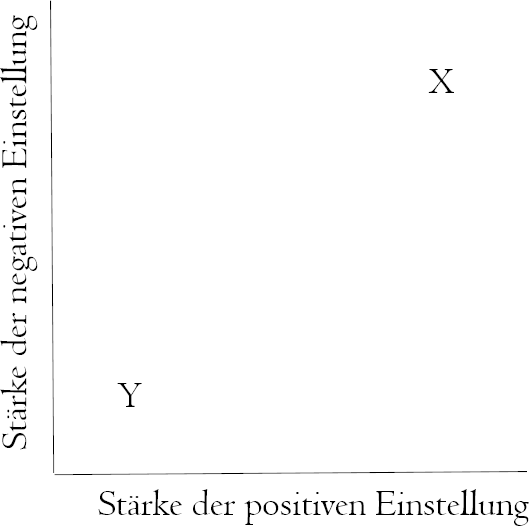
\includegraphics[scale=0.7]{ModellEinstellungen2D} 
\begin{tikzpicture}
    \begin{axis}[axis lines*=left,
                 xtick=\empty,
                 ytick=\empty,
                 ylabel={Stärke der negativen Einstellung},
                 xlabel={Stärke der positiven Einstellung},
                 ylabel near ticks,
                 xlabel near ticks,
                 nodes near coords,
                 point meta=explicit symbolic,
                 enlargelimits=0.25]
        \addplot [black, only marks] coordinates { (0,0) [Y] (1,1) [X] };
    \end{axis}
\end{tikzpicture}
\caption{Zweidimensionale Modellierung von Einstellungen \citep[s.][207]{Jonas.2014}}
\label{pic:2D}
\end{figure}

Es ist schwierig zu sagen, wie die einzelnen Komponenten von Einstellungen genau interagieren und welche Rolle sie jeweils spielen \citep[s.][400]{Lasagabaster.2005}. 
Da die Trennung der drei Komponenten sehr schwer aufrecht zu erhalten ist, wird sie sogar oft insgesamt kritisch gesehen~\citep[s. etwa][34]{Cuonz.2014}. 
Insbesondere was die Verhaltenskomponente von Einstellungen angeht, gibt es in der Forschung unterschiedliche Meinungen dar{\"u}ber, wie eng diese mit den beiden anderen Komponenten zusammenh{\"a}ngt \citep[s.][25]{Garrett.2012}. 
Einerseits kann ein bestimmtes Verhalten dazu führen, dass wir eine bestimmte Einstellung ausbilden, um zu verhindern, dass unser Verhalten und unsere Einstellungen nicht übereinstimmen \citep[s.][203]{Jonas.2014}. 
Andererseits kann aus starken Einstellungen unter bestimmten Voraussetzungen das Verhalten vorhergesagt werden \citep[s.][224--225]{Jonas.2014}. 
Ob eine Einstellung zu einem bestimmten Verhalten führt, hängt aber auch von der Motivation einer Person ab, das Verhalten tatsächlich auszuführen. 
Außerdem spielen die Erwartungen anderer eine Rolle sowie nicht zuletzt die eigene Einschätzung der Fähigkeit, das Verhalten auszuführen (\cites[s.][224--225]{Jonas.2014}[s. auch][]{Ajzen.1977}). 
Die positive Einstellung einer Person zum Dialekt führt also eher dazu, dass sie den Dialekt verwendet, wenn sie dazu motiviert ist, wenn andere von ihr erwarten, dass sie im Dialekt spricht, und wenn sie den Dialekt beherrscht. 
Die \textit{Theory of Reasoned Action} geht deshalb davon aus, dass eher Verhaltensabsichten als das Verhalten selbst Voraussetzung für die Einstellung sind~\citep[s.][26--27]{Garrett.2012}.\largerpage[-1]

Das Verhalten wird in der Sozialpsychologie aufgrund dieser recht komplexen Zusammenhänge nur unter bestimmten Voraussetzungen als Hinweis auf eine bestimmte Einstellung genutzt, n{\"a}mlich dann, wenn die anderen Einstellungskomponenten nur schwach ausgepr{\"a}gt sind oder wenn f{\"u}r ein Verhalten au{\ss}er der Einstellung keine andere Begr{\"u}ndung infrage kommt~\citep[s.][221]{Aronson.2014}. 
Dass es einen gewissen Zusammenhang zwischen Einstellung und Verhalten gibt, ist jedoch die theoretische Voraussetzung dafür, das Ausfüllen eines Fragebogens oder andere Reaktionen auf sprachliche Phänomene als Hinweise auf eine kognitive Einstellung zu deuten \citep[s.][401]{Lasagabaster.2005}.

\citet[78]{Hermanns.2002} zufolge ist die affektive Komponente die zentrale und wichtigste Einstellungskomponente. Auch \citet[222]{Cargile.1994} betonen die Zentralit{\"a}t von Emotionen. Bspw. halten sie es f{\"u}r unwahrscheinlich, dass die kognitive Komponente die affektive {\glqq}{\"u}berstimmt{\grqq} \citep[s.][222]{Cargile.1994}. 
Dies passt zu der Beobachtung, dass es nur sehr selten geschieht, dass affektive Einstellungen durch Argumente ver{\"a}ndert werden~\citep[s.][219]{Aronson.2014}. 
\citet[142]{Riehl.2000} definiert Einstellungen sogar als ausschließlich affektiv. 
Viele dieser Abgrenzungsschwierigkeiten basieren auf der Gleichsetzung der Einstellung selbst mit den Komponenten (s. oben). 
Sieht man diese jedoch wie \citet[]{Jonas.2014} als Voraussetzungen für Einstellungen, wird deutlich, dass bspw. die affektive Komponente keinesfalls allein entscheidend dafür ist, welche Einstellung jemand entwickelt, sondern dass auch die Verhaltenskomponente, vor allem aber das erworbene Wissen die Einstellung prägen.\footnote{Bspw. ist die Einschätzung \citeauthor{Riehl.2000}s (\citeyear[147]{Riehl.2000}), eine Probandin äußere mit ihrer Aussage \object{ich weiß es nicht warum [...] aber grad das heftige sächsisch [...] gefällt mir einfach nicht} eine \glqq rein affektive Zuweisung\grqq{} zu hinterfragen. Da \citet[159]{Riehl.2000} selbst Stereotype als \glqq kognitive Größen\grqq{} sieht, auf denen solche Spracheinstellungen beruhen, ist diese Schlussfolgerung nicht nachvollziehbar.}

Als weitere Schwierigkeit bei der Erforschung von Spracheinstellungen nennen \citet[182]{Plewnia.2011}, dass Einstellungen von den Befragten unterschiedlich stark reflektiert w{\"u}rden \citep[s. auch][143]{Riehl.2000}. 
Das heißt, Einstellungen können sowohl explizit als auch implizit vorhanden sein: 
\begin{quote}Explizite Einstellungen sind solche, die wir bewusst bekr{\"a}ftigen und {\"u}ber die [wir] leicht Auskunft geben k{\"o}nnen; sind das, was wir als unsere Bewertung angeben.~\citep[222]{Aronson.2014}\end{quote}
Implizite Einstellungen hingegen seien viel weniger kontrollierbar und häufig unbewusst \citep[s.][222]{Aronson.2014}. Wie die einzelnen Einstellungskomponenten können sich auch explizite und implizite Einstellungen widersprechen \citep[s.][222]{Aronson.2014}. Das heißt, jemand kann bspw. zwar eine explizit negative affektive Einstellung gegenüber Katzenvideos äußern, aber beim Anschauen dennoch positive Gefühle entwickeln, die eine andere implizite Einstellung verraten.

Die drei Komponenten, Affekt, Kognition und Konation, werden zwar als Voraussetzungen für (implizite und explizite) Einstellungen gesehen, können aber noch nicht erklären, wie es zu einer Einstellung kommt. 
Damit und mit der Frage, welche Aspekte (bspw. welche Gefühle und welche Art von Wissen) für die Herausbildung einer Spracheinstellung relevant sind, beschäftigt sich der folgende Abschnitt. 
\subsubsection{Bewertungsgrundlage und Bewertungskategorien}
\label{sec:Bewertungsgrundlage}
Zu der Frage, wie die Bewertung sprachlicher Formen zustande kommt, gibt es zwei Hypothesen: 
Die \textit{inherent value hypothesis} geht davon aus, dass bspw. phonologische Merkmale f{\"u}r die positive oder negative Bewertung von W{\"o}rtern oder Variet{\"a}ten verantwortlich sind, w{\"a}hrend die \textit{imposed norm hypothesis} davon ausgeht, dass soziale Stereotype und Konnotationen f{\"u}r die Bewertung sprachlicher Formen und Variet{\"a}ten verantwortlich ist~\citep[s.][5]{Garrett.2012}. 
Die erste Hypothese wird allerdings kaum vertreten, da sich gezeigt hat, dass sprachinterne Merkmale für die Bewertung nicht ausschlaggebend sind: 
\begin{quote}[I]t has been shown that listeners rating totally unfamiliar (foreign) varieties (which for respondents were non-categorizable socioeconomically) did not discriminate between them on the ground of aesthetic and status differences, although they were perceived to differ sharply in these qualities within their own speech communities. It seems therefore that evaluations of language varieties do not reflect either linguistic or aesthetic qualities so much as the social conventions within speech communities concerning the status and prestige associated with \so{speakers} of the varieties.~\citep[585, Hervorhebung im Original]{Giles.1988}\end{quote}
Die Bewertung sprachlicher Formen erklärt sich also aus deren Verknüpfung mit sozialen Werten, d.\,h., Spracheinstellungen stellen nicht in erster Linie Reaktionen auf formale Gegebenheiten, sondern 
\begin{quote}gesellschaftlich vermittelte Produkte sozialer Lernprozesse dar und sind als solche entwicklungsf{\"a}hig und ver{\"a}nderbar und in ihrer Aktualisierung von situationsspezifischen Bedingungen abh{\"a}ngig.~\citep[728]{Neuland.1993}\end{quote}
Spracheinstellungen werden also im Laufe der Sozialisation erlernt.\footnote{Man nimmt an, dass Einstellungen, die relativ fr{\"u}h erworben werden, verhältnismäßig stabil sind und nicht so leicht ge{\"a}ndert werden (\citealp[5]{Garrett2003}; s. auch \citealp[30]{Garrett.2012}).}
Dabei spielen Eltern, Freund:innen, Erziehung und Bildung eine wesentliche Rolle \citep[s.][400]{Lasagabaster.2005}.\footnote{Es gibt Studien, die davon ausgehen, dass auch genetische Dispositionen Einstellungen beeinflussen können \citep[s.][400]{Lasagabaster.2005}.} 
\citet[22]{Garrett.2012} sieht als zwei wesentliche Bereiche, aus denen sich Spracheinstellungen speisen, die pers{\"o}nliche Erfahrung und das soziale Umfeld, zu dem er auch die Medien z{\"a}hlt.
Durch sie werden stereotype Vorstellungen {\"u}ber Sprecher:innen vermittelt und mit einer Variante oder Variet{\"a}t in Verbindung gebracht (\cites[s.][180]{Gartig2010}[180]{Plewnia.2011}[37]{Preston2004}). 
Stereotype formen Spracheinstellungen also zu einem großen Teil. 
Ein Stereotyp kann mit \citet{Aronson.2014} verstanden werden als

\begin{quote} 
\sloppy
eine verallgemeinernde Annahme über eine Gruppe von Menschen, die praktisch all ihren Mitgliedern, unabhängig von tatsächlichen Unterschieden zwischen ihnen, dieselben charakteristischen Merkmale zuschreibt. \citep[476]{Aronson.2014} 
\end{quote} 
Stereotype führen zu prototypischen Vorstellungen von Vertreter:innen sozialer Gruppen wie \object{Medizinerinnen sind intelligent} \citep[s.][142]{Riehl.2000}.
Eine solche Annahme zu typischen Eigenschaften oder Verhaltensweisen wird (meist unbewusst) auf sprachliche Merkmale, bspw. Fachbegriffe, übertragen, sodass diese ausreichen, um stereotype Vorstellungen hervorzurufen (\cites[s.][81]{Hundt.1992}[38--39]{Preston2004}). 
Stereotype lassen sich der kognitiven Komponente zuordnen und sind wesentlich für die Herausbildung von Spracheinstellungen \citep[s.][201]{Jonas.2014}. 
Dabei spielen sowohl Heterostereotype, also Vorstellungen über andere Gruppen, als auch Autostereotype eine Rolle, also Vorstellungen über die eigene Gruppe \citep[s.][6--7]{Hundt.1992}. 
Hinzu kommen vermutete Hetero- und vermutete Autostereotype. 
\citet[7]{Hundt.1992} schreibt stereotypen Vorstellungen mehrere Funktionen zu, unter anderem Orientierung und Komplexitätsreduktion. 
Des Weiteren haben Stereotype immer auch eine Selbstdarstellungsfunktion:~Indem ich andere auf eine bestimmte Weise darstelle, positioniere ich mich selbst~\citep[s.][7]{Hundt.1992}. 
\citet[728]{Neuland.1993} f{\"u}hrt deshalb an, dass Spracheinstellungs{\"a}u{\ss}erungen mehr Aufschluss {\"u}ber die Person geben, die diese {\"a}u{\ss}ert, als {\"u}ber das Einstellungsobjekt, also etwa die Variet{\"a}t, da sie insbesondere zur Konstruktion der eigenen Identit{\"a}t und zur Abgrenzung von anderen dienen. 
Spracheinstellungen sind daher gruppenspezifisch \citep[s.][627]{Garrett.2001}. So zeigen \citet{Garrett.1999} etwa, dass walisische Jugendliche andere Einstellungen gegenüber der \textit{Received Pronunciation} (RP) haben als ihre Lehrer:innen. 

Die Bedeutung sozialer Gegebenheiten für Spracheinstellungen schlägt sich in den Kategorien nieder, die bei der Bewertung sprachlicher Merkmale relevant gemacht werden.  
So zeigt sich in bisherigen Studien, dass die wichtigsten Bewertungsaspekte sich in eine Status- und eine Wärmekategorie aufteilen (\cites[s.][155]{Creber.1983}[49]{Preston2004}{Fiske.2002}). 
Zur Statuskategorie gehören Eigenschaften wie Kompetenz und Bildung;  
Eigenschaften wie Freundlichkeit, Gruppensolidarität und Sympathie werden in der Wärmekategorie zusammengefasst~\citep[s.][182]{Plewnia.2011}.
\citet[223--224]{Cargile.1994} nennen zahlreiche Studien, die Evidenz f{\"u}r solche unterschiedlichen Bewertungsdimensionen liefern, wobei nicht immer die gleichen Dimensionen festgestellt werden. \citet{Lambert.1967} etwa unterscheidet zwischen \textit{personal integrity, competence} und \textit{social attractiveness}; 
\citet[117]{Garrett.2007} nennt \textit{superiority, social attractiveness} und \textit{dynamism}. 
Häufig lässt sich ein Zusammenspiel zwischen einer positiven Bewertung in der einen Dimension und einer negativen Bewertung in der anderen Dimension beobachten, sodass Gruppen und die ihnen zugeschriebenen sprachlichen Merkmale entweder als freundlich, sympathisch usw., aber wenig kompetent oder aber als gebildet und professionell, aber unsympathisch empfunden werden \citep[s.][878--879]{Fiske.2002}.
Bei der Bewertung von Variet{\"a}ten zeigt sich als Muster, dass Sprecher:innen die eigene  Nonstandardvariet{\"a}t freundlich, sympathisch und vertrauensw{\"u}rdig, aber langsam und wenig intelligent finden, w{\"a}hrend sie Sprecher:innen der Standardvarietät als kalt, unehrlich, unsympatisch und intelligent empfinden~\citep[s.][1687]{Preston2005}.
% Änderung Anfang
F{\"u}r die Bewertung in Kategorien wie Kompetenz und Bildung ist dabei entscheidend, wie der gesellschaftliche Status der bewerteten Gruppe eingesch{\"a}tzt wird:~Gilt er als hoch, werden Gruppenmitglieder als professionell und kompetent wahrgenommen~\citep[897]{Fiske.2002}.
Die Bewertung in der Wärmedimension hängt \citet[897]{Fiske.2002} zufolge maßgeblich davon ab, ob die bewertete Gruppe als Konkurrenz bzw. als Gefahr für den eigenen Status empfunden wird.
Positive Werte in Status- und Wärmedimension erhalten neben der eigenen \textit{In-Group} insbesondere Gruppen, die in einer Gesellschaft als Referenzgruppe gelten; in den USA bspw. gilt dies laut \citet[898]{Fiske.2002} etwa für die Mittelschicht.
% Änderung Ende

Dass soziale Kategorien die entscheidenden Aspekte der Bewertung sind, heißt allerdings nicht, dass immer bewusst auf diese referiert wird. 
Vordergründig stehen häufig andere Kriterien im Zentrum. 
So zeigt \citeauthor{Preston2004} (\citeyear{Preston1996, Preston2004, Preston2005}), dass sich Befragte vor allem auf die Kategorien Korrektheit und angenehmer Klang beziehen. 
Über die Korrektheit als Bewertungskategorie schreibt er: {\glqq}I personally believe it is no exaggeration to say that it may be the most powerful contributor to awareness in American English{\grqq}~\citep[54]{Preston1996}. 
Solche normativen oder ästhetischen Kriterien sind allerdings eng mit sozialen Kategorien assoziiert. 
Bspw. werden Sprecher:innen der Standardvarietät in Statuskategorien wie Intelligenz h{\"o}her bewertet, w{\"a}hrend Sprecher:innen einer Nonstandardvariet{\"a}t eher bei Eigenschaften wie Vertrauensw{\"u}rdigkeit h{\"o}her bewertet werden~(\citealp[s.][155]{Creber.1983}; sowie \autoref{sec:Prestigevarietaet}). 
Auch \citet[732]{Neuland.1993} stellt fest, dass die Bewertung eines Merkmals als nicht normgerecht h{\"a}ufig mit der Bewertung desselben Merkmals als sympathisch korreliert. 
Auf der anderen Seite kann die Standardvarietät in bestimmten Situationen mit geringer Solidarität assoziiert sein \citep[s.][586--587]{Giles.1988}.

Vor dem Hintergrund dieser Befunde zum Zustandekommen von Spracheinstellungen lässt sich mehr über deren Funktion sagen. 
In der Sozialpsychologie wird zwischen Objekten unterschieden, die eher aufgrund ihres Nutzens beurteilt werden (etwa Klimaanlagen) und Objekten, deren Bewertung auf sozialen Werten beruht (etwa Nationalflaggen) \citep[s.][210]{Jonas.2014}. 
Sprache lässt sich klar dem letzteren Gegenstandstyp zurechnen. 
Ihre Bewertung betrifft die eigene Identität und persönliche Werte: 
\begin{quote} A speaker's language attitudes mirror the norms of the group of people to whom he/she relates most closely, especially when these attitudes and the behaviour which they guide function as group identity markers. This implies that language behaviour has social meaning and prompts social categorization. \citep[1321]{Vandermeeren2005} \end{quote} 
Somit wird deutlich, dass Spracheinstellungen zwar als kognitive Phänomene konzeptualisiert werden können, sich aber nicht losgelöst vom sozialen Kontext betrachten lassen. 
Dies wird im folgenden Abschnitt weiter ausgeführt. 
\subsubsection{Spracheinstellungen im Kontext}
\label{sec:Interaktion}
\citet[72--73]{Hermanns.2002} kritisiert an der sozialpsychologischen Theorie der Einstellungen, dass nicht zwischen abstrakten Typen von Einstellungen und gerade aktualisierten unterschieden wird:
\begin{quote}Ausgelassen bleibt an dieser Stelle der Gedanke, dass man eine virtuelle Einstellung immer erst noch aktualisieren muss, damit sie wirksam sein kann. Wie auch der Gedanke, dass es durchaus aktuelle Bereitschaften zu Arten des Reagierens geben kann, die keinem Typ der gelernten Einstellungen entsprechen.~\citep[73]{Hermanns.2002}\end{quote}
In diesem Zusammenhang weist er auch darauf hin, dass Menschen oft verschiedene Einstellungen ein und derselben Sache gegen{\"u}ber haben, also {\"u}ber Einstellungssets verf{\"u}gen. 
Welche Einstellung aktualisiert % Änderung Anfang
und geäußert % Änderung Ende
wird, h{\"a}ngt dann ma{\ss}geblich vom Kontext ab \citep[73--74]{Hermanns.2002}. 
Entgegen dieser Kritik wird die Kontextabhängigkeit von Einstellungen in der Sozialpsychologie und in der Spracheinstellungsforschung bereits berücksichtigt. 
\citet[210--211]{Jonas.2014} etwa gehen darauf ein, dass die Äußerung einer Einstellung davon abhängig sein kann, wem gegenüber sie getätigt wird. 
Auch wie sich eine Testperson f{\"u}hlt, kann sich auf ihre Einstellungen auswirken~\citep[s.][218]{Cargile.1994}. 

Neuere Arbeiten der Spracheinstellungsforschung betonen, dass Spracheinstellungen in der Interaktion entstehen (\cites[s.][205--206]{Tophinke.2006}[200]{Liebscher.2009}[5--6]{Konig.2014}). \citet{Konig.2014} etwa untersucht Spracheinstellungsäußerungen in konkreten Interaktionen und zeigt, wie metapragmatisches Wissen -- etwa über die Angemessenheit sprachlicher Formen~-- ausgehandelt wird (\cites[s. auch][200]{Konig2015}{Konig.2017}). 
Anhand von Interviewausschnitten zum Sächsischen demonstrieren \citet[206--207]{Liebscher.2009}, dass es sich bei % Änderung Anfang
Spracheinstellungsäußerungen % Änderung Ende
um Positionierungen in den sozialen Strukturen einer konkreten Situation handelt. 
Die Interviewteilnehmer:innen gehen durch ihre Äußerungen etwa in Opposition zu anderen Beteiligten. 
\citet[218]{Liebscher.2009} kommen zu dem Schluss, dass es kontextunabhängige Einstellungen nicht geben kann. 

Auch ältere Studien im Bereich der Spracheinstellungen sehen bereits die Relevanz des Kontextes.
Ein Beispiel ist eine Untersuchung von \citet{Creber.1983}, in der zwölf- bis 14-jährige britische Schüler:innen Standard- und Nonstandardsprecher:innen in einem informellen und einem formellen Setting bewerten sollen. 
Es zeigt sich, dass positive Statuseigenschaften noch stärker mit der Standardvarietät verbunden werden, wenn die Bewertung innerhalb eines formellen Settings stattfindet \citep[s.][159]{Creber.1983}.

In einer nat{\"u}rlichen Interaktionssituation dient nicht nur die Sprache einer Sprecherin als Bewertungsgrundlage, sondern der H{\"o}rer bezieht in sein Urteil auch bspw. die Kleidung, das Auftreten usw. mit ein. 
Sprachliche Merkmale sind in der Interaktion allerdings besonders relevant: \begin{quote} Indeed, contextual issues notwithstanding, we maintain that language behaviours are among the most salient and often used cues in social interaction, and thus the importance of focusing on language attitudes~\citep[215]{Cargile.1994} \end{quote}
Das bereits gewonnene Wissen über ein Gegenüber beeinflusst die Interpretation der sprachlichen Merkmale aber erheblich. 
\citet{Cargile.1994} modellieren die gemeinsame Vergangenheit der Interaktionspartner:innen daher als eine Art Filter, der die Reaktion auf ein sprachliches Verhalten mitbestimmt. 
Spricht bspw. eine gute Freundin mit einem bestimmten Akzent, der sonst als ungebildet empfunden wird, ist diese Interpretation nicht wirksam, wenn die Freundin als intelligent eingesch{\"a}tzt wird \citep[s.][222--223]{Cargile.1994}. 
Auch dies betont die Kontextabh{\"a}ngigkeit von Spracheinstellungen.

%\begin{figure}\includegraphics[width=\textwidth]{Images/Cargile,Gilesetal(2).jpg}\caption{Spracheinstellungsmodell von \citet[214]{Cargile.1994}}
%\label{pic:Cargile}
%\end{figure}
Spracheinstellungen % Änderung Anfang
und die Äußerungen, zu denen sie führen, % Änderung Ende
sind also keineswegs nur kognitiv, sondern insbesondere sozial bedingt, was auch \citet{Aronson.2014} betonen. 
Sie bezeichnen Einstellungen als {\glqq}hochgradig soziales Ph{\"a}nomen, das vom angenommenen oder tats{\"a}chlichen Verhalten anderer Menschen beeinflusst wird{\grqq}~\citep[223]{Aronson.2014}. 
\citet{Garrett.2012} schließt daher:
\begin{quote}[L]anguage attitudes issues extend to all manner of sociolinguistic and social psychological phenomena, such as how we position ourselves socially, and how we relate to other individuals and groups. They may affect behaviours and experiences.~\citep[15]{Garrett.2012}\end{quote}
Spracheinstellungsäußerungen sind damit nicht nur zu einem wesentlichen Teil vom Kontext abhängig, sondern sie wirken auch auf diesen zurück. 
In Interaktionssituationen werden Spracheinstellung% Änderung Anfang
säußerungen und damit auch die Einstellungen selbst % Änderung Ende
daher sowohl als Input als auch als Output gesehen, wie bereits oben in der Diskussion des Zusammenhangs von Verhalten und Einstellungen angeklungen ist (s. \autoref{sec:Komponenten}; \citealp[400]{Lasagabaster.2005}). 
Als Beispiel nennt \citet[21]{Garrett.2012} Einstellungen gegen{\"u}ber dem Walisischen:~Auf der einen Seite k{\"o}nnen positive Einstellungen dazu f{\"u}hren, dass das Walisische erlernt wird (Input), auf der anderen Seite kann das erfolgreiche Erlernen der Sprache zu positiven Einstellungen f{\"u}hren (Output). 
Das bedeutet, dass Spracheinstellungen soziale Realität mitformen. 
Dies zeigt bspw. auch eine Untersuchung von \citet{Keim.1995}, in der es darum geht, wie das sprachliche Verhalten und die Identifikation mit einer lokalen Gemeinschaft zusammenhängen. 
In Narrativen der Proband:innen \citeauthor{Keim.1995}s werden verschiedene Variet{\"a}ten (Dialekt und Standard) zur Konstruktion einer wir-Gruppe in Abgrenzung zu einer fremden, negativ bewerteten Gruppe (bspw. die Vornehmen) verwendet~\citep[s.][170]{Keim.1995}.

Mit dieser Hinwendung zu konstruktivistischen Fragestellungen nähert sich die Spracheinstellungsforschung der Sprachideologieforschung an, deren anthropologisch geprägte Theorie darauf ausgerichtet ist, dem Zusammenhang von sprachlichen und sozialen Kategorien auf den Grund zu gehen. 
\subsection{Sprachideologieforschung}
\label{sec:Sprachideologieforschung}
Der Begriff Ideologie ist in der Alltagssprache meist negativ konnotiert \citep[s.][124--127]{Silverstein1998}. Ideologien werden häufig verstanden als \glqq a system of wrong, false, distorted or otherwise misguided beliefs, typically associated with our social or political opponents\grqq{} \citep[2]{vanDijk.1998}. 
Der anthropologische Ideologiebegriff hingegen meint nicht etwa falsche Vorstellungen, sondern schließt alle Konzeptualisierungen, auch wissenschaftliche, mit ein (\cites[s.][312]{Silverstein1992}[124]{Silverstein1998}). 
Ideologien werden hier urteilsfrei als Systeme von Annahmen und Wertungen gefasst (\cites[s.][3]{vanDijk.1998}[12]{Gal.2019}).\footnote{Die einzelnen Ansätze unterscheiden sich hier durchaus, wie \citet[56--57]{Woolard1994} herausstellen: Während einige grundsätzlich alle Konzeptualisierungen als ideologisch auffassen (hier nennen \citeauthor{Woolard1994} etwa \citealp{Rumsey.1990}), stellen andere die Gefahr der ideologisch verzerrten Darstellung in den Vordergrund und betrachten Ideologien in erster Linie als Mittel, soziale Privilegien zu rechtfertigen.} 
Bei Ideologien handelt es sich um gesellschaftliche Phänomene, das heißt, sie sind immer in einer bestimmten Gruppe verortet und hängen eng mit deren Kultur zusammen (\cites[s.][312]{Silverstein1992}[3]{vanDijk.1998}).

Sprachideologien sind demzufolge Wertehaltungen und Grundeinstellungen einer Gesellschaft zu Sprache und sprachlichen Formen (\cites[s.][]{Silverstein1979}{Silverstein1992}{Silverstein1998}{Kroskrity.2010}{Spitzmuller2013}). 
\citet[193]{Silverstein1979} definiert sie als \glqq any sets of beliefs about language articulated by the users as a rationalization or justification of perceived language structure and use\grqq{}. 
Anders als der sozialpsychologisch geprägten Spracheinstellungsforschung geht es der Sprachideologieforschung also nicht um kognitive Repräsentationen, sondern es wird untersucht, auf welchen grundlegenden Annahmen über Sprache metapragmatische Äußerungen beruhen \citep[s.][223]{Silverstein.1985}. 
Diese sprachideologischen Annahmen können aus expliziten metapragmatischen {\"A}u{\ss}erungen abgeleitet werden, kommen aber noch h{\"a}ufiger implizit zum Ausdruck, indem in bestimmter Weise auf einen Sprachgebrauch reagiert wird~\citep[s.][116]{Gal.2016}.

\begin{sloppypar}
Sprachideologien werden zumindest von einer Gruppe innerhalb einer Sprechergemeinschaft oder aber sogar von der ganzen Sprechergemeinschaft geteilt \citep[s.][125]{Silverstein1998}. 
Welche Sprachideologien in einer Gesellschaft entwickelt und verbreitet werden, h{\"a}ngt dabei zu einem Teil auch davon ab, wie das Sprachsystem aufgebaut ist~\citep[s.][194]{Silverstein1979}. 
Bspw. setzt ein Diskurs über gendergerechte Sprache ein Sprachsystem voraus, in dem die Markierung verschiedener Geschlechter angelegt ist. 
\end{sloppypar}

\begin{sloppypar}
Dass Sprachideologien gesellschaftliche Phänomene sind, zeigt sich daran, dass es im Wesentlichen um den in einer Gruppe angenommenen \glqq Zusammenhang zwischen sprachlicher Variation bzw. Sprachwahl auf der Mikroebene und gesellschaftlich\hyp sozialer Differenzierung auf der Makroebene\grqq{}~\citep[202]{Konig2015} geht. 
Sprachideologien sind also als Verbindungen zwischen sprachlichen Formen und sozialen Strukturen zu verstehen \citep[s.][55]{Woolard1994}. 
Dabei ist wichtig, dass weder die sprachlichen noch die sozialen Kategorien als von sich aus gegeben angenommen werden:
Zum einen sind Sprachideologien entscheidend dafür, wie Sprache konzeptualisiert und kategorisiert wird. 
Zum anderen werden soziale Strukturen und Identit{\"a}ten erst durch (sprachliche) Interaktion und Ideologien darüber konstruiert (\cites[s.][289]{Ochs.1993}[407]{Ochs1996}[70]{Eckert.2016}). 
Ideologien über Sprache wirken daher mit an der Konstruktion sozialer Realität, indem sie sprachliche Formen und Varietäten mit bestimmten Sprecher- oder Kontextmerkmalen verbinden und dadurch spezifische Gruppen oder Situationen häufig erst konstituieren: 
\end{sloppypar}

\begin{quote}[I]t has become clearer that people not only speak about, or refer to, the world “out there” -- outside of language -- they also presuppose (or reflect) and create (or fashion) a good deal of social reality by the very activity of using language.~\citep[194]{Silverstein1979}\footnote{\citeauthor{Silverstein1979} spricht daher nicht von Mikro- und Makroebene, sondern legt den Fokus darauf, wie Kultur diskursiv hervorgebracht wird \citep[s. etwa][]{Silverstein.2013}.}\end{quote}
Soziale Kategorien existieren also nicht losgelöst von Sprache und Vorstellungen darüber, wie Sprache verteilt ist \citep[s.][81--82]{Cameron.1990}. 
Der Zusammenhang zwischen sozialen Identit{\"a}ten und sprachlichen Formen ist dabei immer über Ideologien vermittelt~\citep[s.][288]{Ochs.1993}. 
Für diesen mittelbaren Zusammenhang zwischen Sprache und sozialer Realität spielt die Indexikalität sprachlicher Zeichen eine wesentliche Rolle. Dieses zentrale Konzept der Sprachideologie- oder Metapragmatikforschung ist Thema des folgenden Abschnitts. 

\subsubsection{Indexikalität}
\label{sec:Indexikalitaet}
Sprachliche Variation bietet Sprecher:innen die M{\"o}glichkeit, sich in einer konkreten Situation f{\"u}r eine Variante zu entscheiden. 
Damit ist die Voraussetzung dafür gegeben, diese Entscheidung sprachideologisch zu begründen und die Varianten so sozialsymbolisch aufzuladen~(\citealp[s. u.\,a.][]{Silverstein1979, HessLuttich2005, Eckert2008, Spitzmuller2013}). 
Bspw. werden unterschiedliche Stile oder Varianten oft vereinfachend spezifischen Gruppen zugewiesen und somit auf soziale Unterschiede zur{\"u}ckgef{\"u}hrt. 
In der Folge wird die Nutzung dieser Stile oder Varianten als Hinweis auf die Zugehörigkeit zu der damit assoziierten Gruppe interpretiert. 
Varianten k{\"o}nnen auf diese Weise als Marker sozialer Identität, etwa als weiblich, alt oder Akademikerin fungieren:
\begin{quote} It has become a commonplace in sociolinguistics that linguistic forms, including whole languages, can index social groups. As part of everyday behavior, the use of a linguistic form can become a pointer to (index of) the social identities and the typical activities of speakers.~\citep[36]{Irvine2000}\end{quote}
Indem eine bestimmte Variante verwendet wird, wird also etwas {\"u}ber die soziale Identit{\"a}t ausgesagt -- entweder über die eigene oder über die derjenigen Person, der die Variante in den Mund gelegt wird~\citep[s.][222]{Silverstein.1985}. 
Diese sozialsymbolische Verweiskraft, also \glqq die Fähigkeit sprachlicher Zeichen, soziale Werte, Akteurstypen und Lebensformen zu evozieren bzw. zu kontextualisieren\grqq{} \citep[265]{Spitzmuller2013}, wird in der Sprachideologieforschung als Indexikalität bezeichnet \citep[s.][]{Silverstein1979,Silverstein2003}.\footnote{Unter der Indexikalität sprachlicher Zeichen wird nicht nur der Verweis auf außersprachliche Merkmale verstanden, sondern auch der Verweis auf den Kotext \citep[s.][6--8]{Auer.1995}. \citet[42]{Auer.1989} spricht bei Verweisen auf Außersprachliches von der exophorischen Indexikalität und unterscheidet diese von der endophorischen Indexikalität, womit z.\,B. gemeint ist, dass Wörter durch ihre Endungen auf kongruente Wörter verweisen.}
Dabei kann unterschieden werden zwischen der indexikalischen Form, die in einem sprachlichen Merkmal besteht, dem eine verweisende Kraft zugeschrieben wird, und dem \textit{indexed feature}, einem Kontextmerkmal, auf das verwiesen wird \citep[s.][2]{Auer.1995}.

Die soziale Bedeutsamkeit der Variation sprachlicher Zeichen sollte nicht als bloßer Nebenschauplatz verstanden werden: 
Sie ist ein wesentliches Element von Sprache und häufig zentral für den Ablauf der Kommunikation (\cites[s.][19]{Silverstein.1976}[131]{Gumperz.1982}[68]{Eckert.2016}).\footnote{Während in der Sprachideologieforschung v.\,a. von \textit{Indexikalität} die Rede ist, ist in anderen Teildisziplinen eher der von \citet{Gumperz.1982} geprägte Begriff der \textit{Kontextualisierung} geläufig.}
Ob man bei der Bestellung im Restaurant bspw. den Ausdruck \object{Radler} oder \object{Alster} verwendet, macht nicht nur auf der formalen Ebene einen Unterschied, sondern die Wahl der Variante wird vom Gegenüber als Zeichen der regionalen Herkunft interpretiert. 
Den Zeichengebrauch einer Person als indexikalisch zu interpretieren bedeutet jedoch nicht, eine Intentionalität zu unterstellen \citep[s.][78]{Eckert.2016}. 
Da Sprachideologien meist nicht reflektiert werden, geschieht die Wahl einer Variante in den meisten Fällen unbewusst. 
Möglich ist auch, dass eine Form zun{\"a}chst bewusst eingesetzt wird und dann mit der Zeit in einen automatischen Gebrauch {\"u}bergeht~\citep[s.][79]{Eckert.2016}.

Jedes formale Merkmal einer Sprache kann theoretisch indexikalisch aufgeladen werden (\cites[s.][42]{Silverstein.1976}[206]{Silverstein1979}). 
Dabei können zwei Typen indexikalischer Tokens unterschieden werden: solche, bei denen die indexikalische Bedeutung Teil der Denotation ist, wie etwa Deiktika, und solche, bei denen die Denotation unabhängig von der Indexikalität ist (\cites[s.][34]{Silverstein.1976}[497]{HessLuttich2005}).\footnote{\citet[3]{Auer.1995} weist darauf hin, dass häufig lediglich diejenigen indexikalischen Zeichen in den Fokus der pragmatischen Linguistik gerückt wurden, deren Denotation ohne die Berücksichtigung des Kontextes nicht bestimmt werden kann.}
Letzteres wird besonders gut an Wortpaaren wie \object{Personenkraftwagen} und \object{Auto} deutlich, die zwar die gleiche Denotation aufweisen, denen aber unterschiedliche Indexikalitäten zugeschrieben werden. 
\citet[30--31]{Silverstein.1976} nennt als Beispiel Sexusmarker der Muskogee-Sprachen, die anzeigen, ob eine Aussage von einer Sprecherin oder einem Sprecher ge{\"a}u{\ss}ert wird.
Ein weiteres Beispiel sind die lange und kurze Genitivendung im Deutschen (\object{Baums/Baumes}): Beide tragen die gleiche grammatische Bedeutung, die lange Endung ist aber mit mehr Prestige aufgeladen \citep[s.][]{Szczepaniak2014}.\footnote{Prestige kann mit \citet{Strasser2005} verstanden werden als {\glqq}die Wertschätzung, die einer Person oder Gruppe aufgrund von positiv bewerteten Eigenschaften, wie berufliche Position oder Clubmitgliedschaft, entgegengebracht wird{\grqq}~\citep[412]{Strasser2005}. Stigma bezeichnet komplementär dazu die Abwertung einer Gruppe oder Person \citep[s.][412]{Strasser2005}.}
Solche Zeichen verfügen neben ihrer inhaltsseitigen Bedeutung über davon unabhängige, indexikalische Bedeutungsaspekte, die sich bspw. auf die Kontexte beziehen, in denen sie verwendet werden, oder auf Sprechertypen, mit denen sie assoziiert sind~\citep[s.][206--207]{Silverstein1979}. 
Hier trägt die indexikalische Funktion des Zeichens nicht zur Proposition bei, sondern operiert auf der Ebene des Kontextes. 

\textcites[33--35]{Silverstein.1976}[195--196]{Silverstein2003} beschreibt zwei Seiten der Indexikalität einer Form, die er \textit{presupposition} und \textit{entailment}\footnote{Anstatt von \textit{entailment} spricht \citeauthor{Silverstein1979} z.\,T. auch von \textit{creativity} oder von einem kreativen Effekt (\cites[s.][]{Silverstein.1976}[]{Silverstein1979}).} nennt: 
Mit \textit{presupposition} ist gemeint, dass eine Form bestimmte Kontextmerkmale voraussetzt. 
Ihr Auftreten und ihr Verständnis sind nur möglich, wenn bestimmte Voraussetzungen erfüllt sind. 
Deutlich wird dies insbesondere bei indexikalischen Zeichen, die nur mithilfe des Kontextes interpretierbar sind, wie etwa deiktische Ausdr{\"u}cke (bspw. \object{dieses} in \object{probier mal dieses Kabel})~\citep[s.][33]{Silverstein.1976}. 
Damit geht es bei der \textit{presupposition} auch um die Angemessenheit eines Zeichens im bis zu diesem Punkt etablierten Kontext \citep[s.][195]{Silverstein2003}. 

Der Begriff des \textit{entailment} zielt darauf ab, dass durch die Verwendung einer  Form in einer Situation die Merkmale des Kontextes erst sichtbar gemacht werden. Hier geht es um die Wirkung des Zeichens im Kontext:

\begin{quote} In some cases, the occurrence of the speech signal is the only overt sign of the contextual parameter, verifiable, perhaps, by other, cooccurring behaviors in other media, but nevertheless the most salient index of the specific value. Under these circumstances, the indexical token in speech performs its greatest apparent work, seeming to be the very medium through which the relevant aspect of the context is made to “exist.” \citep[34]{Silverstein.1976}
\end{quote}
Bspw. kann die Äußerung \object{wenn du alles aufisst...} je nach Intonation entweder als Drohung oder als Äußerung einer Bedingung aufgefasst werden. 
Die Intonation verweist also indexikalisch auf eine bestimmte Praktik und kann über diese Indexikalität zu einer bestimmten Interpretation führen \citep[s.][421]{Ochs1996}. 

Für das \textit{entailment} des indexikalischen Zeichens ist entscheidend, welche Implikationen die Verwendung im zuvor etablierten Kontext mit sich bringt \citep[s.][195]{Silverstein2003}. 
So könnte ein umgangssprachlicher Ausdruck in einem Vortrag humoristisch wirken, in einer anderen Situation unter Umständen aber als unhöflich empfunden werden. 
Die Verwendung einer indexikalischen Form wirkt sich außerdem wiederum auf die Erwartbarkeit und Angemessenheit anderer Zeichen aus. 
In einer E-Mail, die man aufgrund einer förmlichen Anrede und eines offiziellen Inhalts als formell wahrnimmt etwa, erwartet man eine Abschiedsformel wie \object{mit freundlichen Grüßen}. 
Diese Erwartungshaltung wird metapragmatisch verhandelt und durch Sprachideologien gestützt \citep[s.][196]{Silverstein2003}. 

Wichtig ist also, dass nicht davon ausgegangen werden kann, dass Kontext oder Kotext das Auftreten eines Zeichens determinieren, sondern dass die Wahl oder Nichtwahl eines Zeichens auch zur Kontextualisierung, also zur Gestaltung des Kontextes beiträgt (\cites[s.][23]{Auer.1986}[42--43]{Gumperz.1992b}).\footnote{In der Soziolinguististik wurde nichtsdestotrotz lange Zeit ein deterministischer Ansatz verfolgt und versucht, von einem Zeichen auf seine Benutzer:innen zu schließen \citep[s.][88--90]{Eckert2012}.
Unterschiede in der Variantenwahl wurden mit höherem bzw. geringerem Planungsaufwand oder mit sozialer Herkunft erklärt \citep[vgl. etwa die Kaufhausstudie von][]{Labov2006}.
\citet{Eckert2012} macht drei Phasen der variationslinguistischen Forschung aus und zählt Studien wie die \citeauthor{Labov2006}s zur ersten Phase.
Studien der zweiten Phase hingegen verfolgten einen ethnografischen Ansatz und berücksichtigten sprachideologische Fragestellungen, hielten sich aber immer noch an vorgefertigte Kategorien wie soziale Klasse \citep[s.][93]{Eckert2012}. Die dritte Phase schließlich brachte eine Fokussierung auf die stilistischen Praktiken der Sprachbenutzer:innen und deren sich wandelnde sozialsymbolische Bedeutungen, betont also die Agentivität der Sprecher:innen.} 
Variation wird damit als komplexes Zeichensystem verstanden \citep[s.][92]{Eckert2012}.
Für die Sprachideologieforschung und die Theorie der Indexikalität ist diese konstruktivistische Sichtweise zentral.

Wie oben bereits erwähnt, entsteht die indexikalische Bedeutung einer Variante nicht ad hoc, sondern wird in der Interaktion ausgehandelt. 
Beide Seiten des {in\-dexi\-ka\-li\-schen} Zeichens (also das bilaterale Zeichen aus Form- und Funktionsseite und die Kategorie, auf die dieses indexikalisch verweist) existieren zunächst unabh{\"a}ngig voneinander und werden erst über den metapragmatischen Diskurs verbunden (\cites[s.][316]{Silverstein1992}[86]{Jaffe.2016}). 
Sobald eine Variante metapragmatisch reflektiert wird, können ihr indexikalische Bedeutungen zugeschrieben werden.\footnote{Diese Zuschreibung sozialer Bedeutsamkeit zu einem zuvor als auffällig wahrgenommenen Merkmal entspricht dem, was \citeauthor{Purschke2014} unter Pertinenz fasst (s. \autoref{sec:MetapragmatischeBewusstheit}). Er betrachtet daher den {\glqq}Gegenstand von Hörerurteilen über Sprache [...] als die salienz- und pertinenzbasierte sozio-pragmatische Indexikalität lebensweltlicher Phänomene{\grqq}\citep[44]{Purschke2014}.} 
Auf diese Weise schaffen Sprachideologien Verbindungen zwischen sozialen Strukturen und sprachlichen Formen \citep[s.][55]{Woolard1994}. 
Dieser Prozess, in dem Formen bestimmte Bedeutungen zugeordnet werden, lässt sich mit \citet[86]{Jaffe.2016} als Indexikalisierung beschreiben und hängt eng zusammen mit dem Prozess der Registrierung \citep[s.][]{Agha2007}, auf den weiter unten eingegangen wird.

\citeauthor{Silverstein1979} (u.a. \citeyear{Silverstein1979}, \citeyear{Silverstein2003}) spricht von verschiedenen aufeinanderfolgenden indexikalischen Stufen bzw. Ordnungen (s. \autoref{pic:Indexikalitaet}). 
Auf der ersten Stufe (\textit{first-order-indexicality}) befinden sich Varianten, deren gruppen-, varietäten- oder registerspezifische Distribution zwar empirisch beobachtbar, den Sprecher:innen aber nicht bewusst ist \citep[s.][265]{Spitzmuller2013}.
Der Bezug der sprachlichen Form zu außersprachlichen Gegebenheiten bleibt hier von der Sprachgemeinschaft unbemerkt und ließe sich lediglich etwa durch Korpusuntersuchungen feststellen.
Auf der zweiten Stufe (\textit{second-order-indexicality}) stehen Varianten, die von Sprecher:innen als Kontextualisierungshinweise im Sinne \citeauthor{Gumperz.1982}' (\citeyear{Gumperz.1982}; s. auch \citealp{Auer.1986}) wahrgenommen werden. 
Kontextualisierungshinweise helfen Teilnehmer:innen einer Interaktion, zu interpretieren, {\glqq}what the activity is, how semantic content is to be understood and \textit{how }each sentence relates to what precedes or follows{\grqq}~\citep[131, Hervorhebung im Original]{Gumperz.1982}. 
Von Seiten der Sprachbenutzer:innen wird dabei häufig auch eine quantitative Verteilung angenommen, die durch außersprachliche Gegebenheiten gesteuert ist und dadurch auf diese verweist \citep[s.][266]{Spitzmuller2013}. 

Auf der Stufe der dritten indexikalischen Ordnung (\textit{third-order-indexicality}) entspricht das Zeichen einem Labovschen Stereotyp\footnote{\citet[52]{Silverstein.2016} weist selbst darauf hin, dass die Unterscheidung \citeauthor{Labov1963}s auf die Idee der indexikalischen Ordnungen übertragbar ist.}, das sich zur Stilisierung bestimmter Personengruppen oder kommunikativer Praktiken eignet (\cites[s.][308--309]{Labov1978}[220]{Silverstein2003}[92]{Eckert2012}). 
So wird etwa die Koronalisierung von [ç] bspw. in \object{ich} oder \object{dich} als ein typisches Merkmal in Äußerungen jugendlicher Sprecher:innen aus einem multikulturellen, großstädtischen Milieu gesehen und dazu verwendet, diese Gruppe zu konstruieren und stereotyp darzustellen (\cites[s.][]{Androutsopoulos.2011}[11]{Auer2014}). 
\citet[523]{Harnisch.2005} sieht insbesondere in morphologischen Varianten ein großes Potenzial, als soziale Marker genutzt zu werden. 
Er nennt etwa verbalmorphologische Klammergef{\"u}ge des unterfr{\"a}nkischen Dialekts (\textit{nei-lass-fall} \glq hineinfallen lassen\grq), dessen Sprecher:innen wegen dieses auff{\"a}lligen Merkmals teilweise mit Bildungen wie \textit{foto-lass-grafieren }verspottet werden, oder genderneutrale Partizipialformen wie \textit{Studierende}, die f{\"u}r politische Korrektheit und Feminismus stehen~\citep[s.][524]{Harnisch.2005}.

\begin{figure}
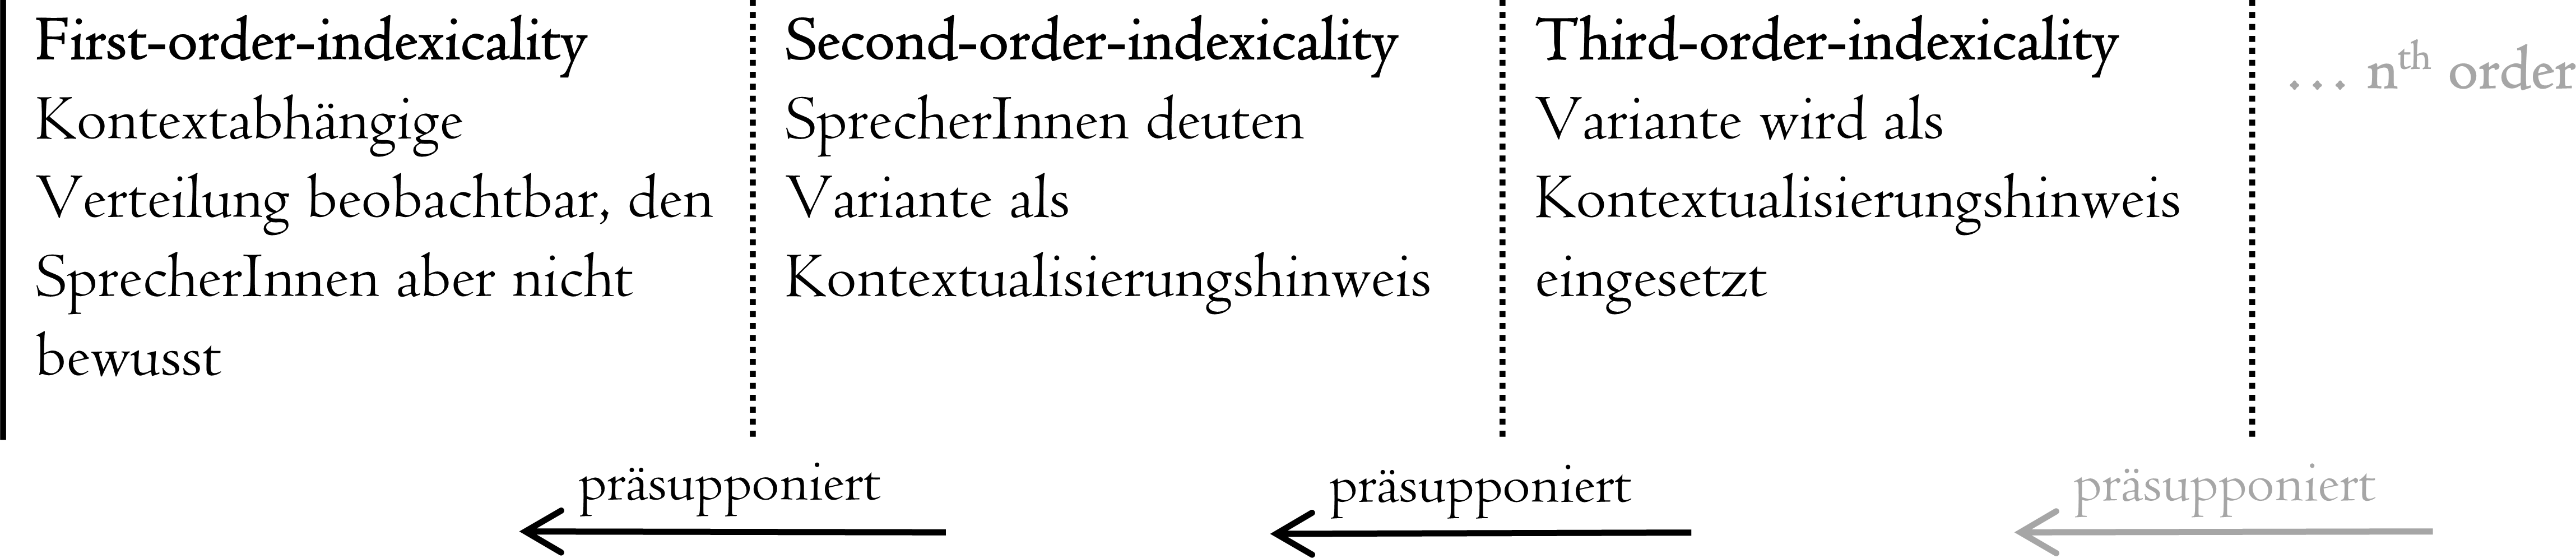
\includegraphics[width=\textwidth]{indexikalischeStufen}
\caption{Indexikalische Stufen nach \citet[]{Silverstein2003}}
\label{pic:Indexikalitaet}
\end{figure}

Wichtig ist, dass die zweite und dritte Ordnung nicht auf einer tatsächlich beobachtbaren Verteilung aufbauen müssen, wie \citet[266]{Spitzmuller2013} betont: \glqq Jede n-te Ordnung präsupponiert die n--1-te Ordnung, was aber nicht bedeutet, dass diese n--1-te Ordnung faktisch wirklich existiert\grqq. 
Studien, die quantitativ untersuchen, welche Gruppe eine Variante h{\"a}ufiger verwendet, k{\"o}nnen daher keinen Aufschluss dar{\"u}ber geben, mit welcher sozialsymbolischen Bedeutung eine Variante aufgeladen ist~\citep[s.][455]{Eckert2008}. 

Da die Verweiskraft in der Interaktion immerzu kreativ genutzt, thematisiert und explizit oder implizit verhandelt wird, ist das System der indexikalischen Ordnungen nach oben offen. 
Sowohl jede Verwendung des Zeichens in einem neuen Kontext als auch die metapragmatische Reflexion tragen zum indexikalischen Gehalt des Zeichens und damit zur weiteren Indexikalisierung bei. 
Das heißt, der Indexikalisierungsprozess ist nie abgeschlossen, sondern die Indexikalität eines Zeichens unterliegt einer ständigen Wandelbarkeit: 

\begin{quote}Variation constitutes a social semiotic system capable of expressing the full range of a community's social concerns. And as these concerns continually change, variables cannot be consensual markers of fixed meanings; on the contrary, their central property must be indexical mutability.~\citep[94]{Eckert2012}
\end{quote}
Auf die dritte indexikalische Stufe können also potenziell beliebig viele weitere Stufen folgen, wie in \autoref{pic:Indexikalitaet} angedeutet~\citep[s.][438]{Woolard2008}.
Sobald eine sprachliche Form einmal von den Sprachbenutzer:innen bemerkt und mit sozialsymbolischer Bedeutung aufgeladen wird, entfaltet sie das Potenzial, mit dem Wissen um die Indexikalität wiederverwendet zu werden und so weitere Bedeutungsfacetten anzunehmen. 
Ein Beispiel, das \citet[13--14]{Eckert.2011} nennt, ist die Realisierung des englischen Phonems \mbox{/θ/} als [t], die in den USA zunächst ein Marker für ethnische Gruppen mit bspw. deutscher oder mexikanischer Herkunft war. 
Auf der nächsten Stufe beinhaltete die Indexikalität dieser Aussprachevariante stereotype Vorstellungen über diese sozialen Gruppen und wurde etwa als Marker für harte Arbeit auf dem Feld gesehen \citep[s.][13]{Eckert.2011}. 
Aufgrund dieser stufenweisen Entwicklung handelt es sich bei indexikalischen Verweisen auf soziale Kategorien oft nicht um einen direkten Verweis der Varianten auf die soziale Kategorie, sondern ein sprachliches Merkmal verweist bspw. indirekt auf eine Gruppe, indem es mit bestimmten Kommunikationspraktiken assoziiert ist, die als typisch für diese Gruppe verstanden werden, oder -- wie im Beispiel von \citet{Eckert.2011} -- andersherum~(\citealp[s.][455]{Eckert2008}; vgl. auch \citealp{Silverstein.1985, Ochs1996}). 

Auf diese Weise kann ein sprachliches Zeichen ein Set an verschiedenen Indexikalitäten entwickeln. 
Um dieser Varianz im Spektrum der indexikalischen Bedeutungen Rechnung zu tragen, entwickelt \citet{Eckert2008} die Idee der indexikalischen Felder, die davon ausgeht, dass eine Variante nicht nur eine Interpretation zulässt, sondern über ein Set von sozialsymbolischen Bedeutungsaspekten verfügt, die je nach Verwendungskontext und beteiligten Akteur:innen aktiviert werden. 
Welcher Aspekt in den Vordergrund rückt, ist dabei sowohl von der Hörerin bzw. dem Leser als auch vom Kotext und dem Inhalt der Äußerung abhängig (\citealp[s.][466]{Eckert2008}; vgl. auch \cites[45]{Gumperz.1992b}[414]{Ochs1996}). 
Als Beispiel nennt \citet[72]{Eckert.2016} das zentralisierte [ɐɪ] aus \citeauthor{Labov1963}s \citeyear{Labov1963} Vineyard-Studie: {\glqq}Once the centralized nucleus indexed an anti-incursion stance on the Vineyard, it was available for reuse, for example, indexing a strong stance on some other issue{\grqq}~\citep[72]{Eckert.2016}.
Je länger eine Variation besteht, desto differenzierter können die indexikalischen Bedeutungsaspekte der Varianten sein \citep[s.][471]{Eckert2008}.

Die Sozialisation der Kommunikationsteilnehmer:innen ist ein wesentlicher Faktor dafür, welche indexikalische Bedeutung ein Zeichen für sie transportiert: 
Als sprachideologische Zuschreibung ist die Indexikalität sprachlicher Varianten sozial stratifiziert \citep[s.][265]{Spitzmuller2013}. 
Die indexikalischen Bedeutungen (bspw. Situation, Zeit, soziale Praktik etc.) werden im Laufe der Sozialisation  mit bestimmten Formen (bspw. Passivformen, Pronomen, bestimmte Fragetypen etc.) verkn{\"u}pft~\citep[s.][410--411]{Ochs1996}.
Auch wenn Kotext, Kontext und Erfahrung aus der eigenen Sprachpraxis das Bedeutungsspektrum der indexikalischen Felder eingrenzen, bleibt die Indexikalität aber immer unscharf, sodass, wie \citet[12--13]{Auer.1995} hervorhebt, zwei Teilnehmer:innen einer Kommunikationssituation den Verweis nie mit den gleichen Worten paraphrasieren würden. 

\begin{sloppypar}
Wie ausdifferenziert die indexikalischen Bedeutungen eines Zeichens sein können, wird an einem weiteren Beispiel deutlich, das \citet[465--466]{Eckert2008} nennt, nämlich den Assoziationen, die die beiden Aussprachevarianten des englischen Suffixes \{-ing\}  hervorrufen. 
Wie Untersuchungen von \citeauthor{CampbellKibler.2007} (\citeyear{CampbellKibler.2005}, \citeyear{CampbellKibler.2007}, \citeyear{CampbellKibler.2008}) zeigen, werden mit den Aussprachevarianten [ɪŋ] und [ɪn] recht unterschiedliche Eigenschaften verbunden. 
\citet{CampbellKibler.2007} lässt in Gruppeninterviews und in einer Umfrage US-amerikanische  Studierende Sprachaufnahmen unterschiedlicher Sprecher:innen bewerten. 
Die natürlichen Aufnahmen werden so manipuliert, dass pro SprecherIn eine Aufnahme mit der Realisierung des Morphems als [ɪŋ] und eine mit der Realisierung als [ɪn] vorliegt. 
Zum einen werden die Varianten als Verweise auf die Herkunft der Sprecher:innen gedeutet: Während [ɪŋ] allgemein der Großstadt zugeordnet wird, gilt [ɪn] als Variante aus Akzenten der Südstaaten \citep[s.][]{CampbellKibler.2007}. 
Zum anderen können die Varianten unterschiedliche Assoziationen mit Sprechertypen hervorrufen: So wird einer der Sprecher, für den die Proband:innen eine großstädtische Herkunft annehmen, signifikant häufiger als homosexuell eingeschätzt, wenn er die Variante [ɪŋ] verwendet \citep[s.][50]{CampbellKibler.2007}. 
[ɪŋ] kann außerdem zu einer höheren Einschätzung der Bildung der Sprecher:innen führen \citep[s.][46--47]{CampbellKibler.2007}. 
[ɪn] hingegen wird unter anderem mit niedriger Bildung und ländlichen Gebieten in Verbindung gebracht. 
Welche Interpretation zum Tragen kommt, ist dabei unter anderem stark von der beurteilenden Person abhängig: 
\end{sloppypar}

\begin{quote} One’s \object{-ing} use is seen by some as more intelligent and by others as annoying, less intelligent, and trying to impress. Another’s \object{-in} guise is seen as compassionate by some and as condescending by others, while a third, when using \object{-in}, is seen by some as annoying and less masculine, while others describe him as a masculine “jock.” \citep[637]{CampbellKibler.2008} \end{quote}
Die Studie \citeauthor{CampbellKibler.2008}s macht deutlich, dass sich die verschiedenen Bedeutungsmöglichkeiten einer Variante durchaus widersprechen können \citep[vgl. auch][93--94]{Jaffe.2016}. 
Offenbar ist für die Interpretation unter anderem entscheidend, ob (aufgrund von Kontext und Kotext) angenommen wird, dass eine Variante Teil des \glqq natürlichen\grqq{} Sprachgebrauchs einer Person ist, oder ob davon ausgegangen wird, dass die Variante bewusst eingesetzt wird, um einen bestimmten Effekt zu erzielen \citep[s.][640]{CampbellKibler.2008}. 
Das Aufzeigen differenzierter indexikalischer Felder macht auch deutlich, dass die häufig vorgenommene Unterteilung in eine {Pres\-tige\-variante} und eine stigmatisierte Variante meistens stark vereinfachend ist \citep[s.][226]{Eckert2004}. 

Einzelne oder mehrere Indexikalitäten können Zeichen mit anderen Zeichen gemeinsam haben, sodass diese Zeichen über ihre indexikalischen Bedeutungen untereinander verbunden sind. 
So kann ein Set von über die Indexikalität vernetzten Sprachzeichen ein sprachliches Register bilden. 
Register lassen sich im linguistisch-anthropologischen Verständnis als ein Repertoire von Zeichen verstehen, das über Sprachideologien mit bestimmten kommunikativen Praktiken und deren Akteur:innen verknüpft ist (\cites[s.][216]{Agha.1999}[38]{Agha2005}). 
Auch sie werden also im metapragmatischen Diskurs konstruiert \citep[s.][46]{Agha2005}. 
Der Prozess dieser sprachideologischen Konstruktion von Registern wird als Registrierung oder \textit{Enregisterment} bezeichnet (s. \cites[231]{Agha2003}[268]{Spitzmuller2013}{Anderwald.2017}). 
Dabei werden Varianten durch ihren Gebrauch sowie durch metapragmatische Kommentare bspw. einer Fachsprache, einer Textsorte etc. zugeordnet \citep[s.][218]{Agha.1999}. 
Die Herausbildung einer Standardsprache etwa ist als Registrierungsprozess zu fassen, an dem verschiedene soziale Akteure, wie etwa Schulen, die Medien usw. beteiligt sind (\cites[s.][64]{Woolard1994}{Auer.2013}). 
Auch das Entstehen von W{\"o}rterb{\"u}chern, Grammatiken und Sprachpflegevereinen tr{\"a}gt zur Registrierung einer Standardsprache bei~\citep[s.][164]{Gal.2006b}.

\begin{sloppypar}
Eine klare Trennung in Register als situationsspezifische Sprachgebr{\"a}uche und Variet{\"a}ten, die bestimmten Personen oder Personengruppen zugeschrieben werden, ist aufgrund der Menge an interagierenden Faktoren und der engen Verwobenheit der Indexikalit{\"a}ten kaum m{\"o}glich \citep[s.][120--121]{Eckert2005}. Vielmehr sind über den Registerbegriff verschiedene Kriterien miteinander verbunden: {\glqq}In all cases, a cultural model associates speaker types, their typified features, activities, practices, and values with a way of speaking: a register{\grqq}~\citep[117]{Gal.2016}. 
Dabei soll die Registrierung einer Form hier nicht mit ihrer Indexikalisierung gleichgesetzt werden:
Bspw. können die verschiedenen Formen, die dem Repertoire der Standardsprache zugeordnet sind, über ganz unterschiedliche Indexikalitäten verfügen \citep[s.][122]{Eckert2005}. 
Möglicherweise verweisen einige Formen des Repertoires auf Bildung, während andere als literatursprachlich oder altmodisch gelten.
\end{sloppypar}

Aus den Konzepten der Indexikalität und der Registrierung ergibt sich, dass es sich bei sprachlichen Varianten oder verschiedenen Stilen keineswegs schlicht um verschiedene Arten handelt, das Gleiche auszudrücken (\cites[s.][28]{Auer.1989}[88]{Coupland.2007}). 
\citet[96]{Eckert2012} konstatiert: \glqq style is at its foundation ideological, and the stylistic form of propositions is very much a part of their meaning\grqq.
Die indexikalische Bedeutung eines Zeichens ist dabei nicht statisch, sondern wird über den Diskurs vermittelt und ständig weiterentwickelt. 
\subsubsection{Ausblendung, fraktale Rekursivität und Ikonisierung}
\label{sec:Prozesse}
% Andersherum kann es auch vorkommen, dass vorhandene soziologische Unterschiede und der Wunsch nach Differenzierung dazu f{\"u}hren, dass sprachliche Variation verst{\"a}rkt wird~\citep[s.][39]{Irvine2000}.
\citeauthor{Irvine2000} (\citeyear{Irvine2000}, \citealp[s. auch][]{Gal.1995} \citeyear[und][]{Gal.2019}) machen drei wesentliche Prozesse aus, die bei sprachideologischen Konzeptualisierungen eine Rolle spielen:~Ausblendung, fraktale Rekursivit{\"a}t und Ikonisierung. 
Sie können die Indexikalität und den Registrierungsprozess stützen und stellen wichtige Faktoren bei der Wahrnehmung sprachlicher Variation dar.
Damit bilden die drei von \citet{Irvine2000} beschriebenen Prozesse gewissermaßen die diskursiven Dynamiken, unter denen Indexikalisierungs- und Registrierungsprozesse entstehen. 

%Ausblendung
\begin{sloppypar}
Der Prozess der Ausblendung (\textit{erasure}) f{\"u}hrt nicht prim{\"a}r dazu, dass ein sprachliches Element oder seine Eigenschaften tats{\"a}chlich ausgel{\"o}scht werden; vielmehr werden sie im Diskurs nicht wahrgenommen oder mit Behelfserkl{\"a}rungen ins Bild eingepasst \citep[s.][38]{Irvine2000}.   
Dies zeigt sich bspw. in einer Untersuchung von \citet{Auer.2017} zum Gebrauch verschiedener Dialektmerkmale am Oberrhein. 
Für dieses Gebiet wurde in der Dialektologie lange angenommen, dass die Dialektgrenze quer zur deutsch-französischen Staatsgrenze verläuft.
Isoglossen, die sich entlang der Staatsgrenze erstrecken und diesem Bild damit widersprechen, wurden ausgeblendet \citep[s.][29]{Auer.2017}. 
Diese Vernachlässigung bestimmter {Va\-rian\-ten\-ver\-tei\-lungen} war vor allem politisch motiviert: \citet{Auer.2017} zitieren insbesondere \citet{Maurer.1942} und merken an: 
\begin{quote} Es bedarf kaum der Erwähnung, dass diese Einschätzung in einem 1942 erschienenen Buch, das \glqq unseren Kameraden an der Front und bei der Wehrmacht\grqq{} gewidmet war, auch ein politisches Statement war. Maurers Darstellung der \glqq Rheinstaffeln\grqq{} [...] ist nicht zuletzt durch die geschickte Wahl der Merkmale bedingt.~\citep[29]{Auer.2017}\end{quote}
Im Metasprachdiskurs {\"u}ber die Sekund{\"a}rpr{\"a}positionen l{\"a}sst sich die ideologische Ausblendung der urspr{\"u}nglichen Dativpr{\"a}positionen und ihres Wandels zum Genitiv beobachten: Sprachbenutzer:innen gehen oft davon aus, dass die Genitivrektion grundsätzlich die ältere Form darstellt \citep[s.][46]{Szczepaniak2014}. 
Teilweise gehen infolge der ideologischen Ausblendung sprachliche Elemente aber auch tatsächlich aus einer Variet{\"a}t oder Sprache verloren \citep[s.][38--39]{Irvine2000}.
\end{sloppypar}

%fraktale Rekursivität
Mit fraktaler Rekursivit{\"a}t beziehen sich \citet[38]{Irvine2000} auf die Beobachtung, dass Unterscheidungen, die auf einer Ebene getroffen werden, auf eine andere Ebene projiziert werden. 
Bspw. wird von vielen Sprachkritiker:innen zwischen \glqq gutem\grqq{} und \glqq schlechtem\grqq{} Deutsch unterschieden. 
Zu letzterem werden häufig Anglizismen gezählt. 
Innerhalb der Gruppe der Anglizismen wird allerdings wieder unterschieden zwischen solchen, die eine Lücke im Wortschatz füllen, und daher als notwendig erachtet werden (etwa \object{Internet}) und solchen, die (scheinbar) eine Entsprechung im Deutschen haben\footnote{Meistens handelt es sich hier lediglich um partielle Synonyme oder Anglizismus und Erbwort entsprechen sich zwar auf der denotativen Ebene, verfügen aber über unterschiedliche Indexikalitäten und werden daher von unterschiedlichen Personengruppen/in unterschiedlichen Kontexten gebraucht \citep[s. hierzu][]{Spitzmuller.2007}.}, und daher als überflüssig und unerwünscht betrachtet werden (etwa \object{Party}). 
Zu einer Opposition werden also Unterkategorien gebildet, die sich wieder gegen{\"u}berstehen. 
Im Falle der Kasusschwankungen bei Sekund{\"a}rpr{\"a}positionen könnte sich die Rekursivit{\"a}t wie folgt zeigen:~Die Sprachbenutzer:innen differenzieren zwischen verschiedenen sozialen Gruppen, bspw. Akademiker:innen und Nichtakademiker:innen. Diese Unterscheidung wird auf Unterschiede zwischen Kommunikationspraktiken und Registern projiziert, etwa dienstliche formelle E-Mails im Gegensatz zu informellen mündlichen Gesprächen. 
Diesen unterschiedenen Registern werden die wahrgenommenen Varianten der Kasusrektion, Genitiv- und Dativrektion zugeordnet~(s. \autoref{sec:IndexikalitaetRektionskasus}).

%Ikonisierung
Mit Ikonisierung ist gemeint, dass ein sprachliches Merkmal als so charakteristisch für eine soziale Gruppe oder einen Kommunikationskontext angesehen wird, dass es geradezu als Stellvertreter für diese bzw. diesen angesehen wird. 
In der Wahrnehmung der Sprecher:innen entsteht ein Abbildverh{\"a}ltnis zwischen dem sprachlichen Merkmal und einem au{\ss}ersprachlichen Merkmal~\citep[s.][37]{Irvine2000}. 
Dadurch rücken Bezeichnetes und Bezeichnung näher zusammen, sodass sich die Zeichenhaftigkeit ein Stück weit auflöst und die Verbindung naturalisiert wird. 
Bspw. wird Sprache als Abbild für Nationalität gesehen, eine Ideologie, die auf Herder zurückgeht \citep[s.][60]{Irvine2000}. 
Hier wird ein Ähnlichkeitsverhältnis (bzw. ein Gleichheitsverhältnis) zwischen der Ausdehnung einer Sprache oder Varietät und der Ausdehnung eines Volkes angenommen. 
Auf Grundlage dieser Sprachideologie wurden während der Kolonialzeit Gebiete anhand von (vermeintlich eindeutigen) Sprachgrenzen eingeteilt, wie \citet[48--49]{Irvine2000} am Beispiel Westafrikas zeigen. 
Als ikonisch kann auch der Gebrauch von Majuskeln bis zur vollständigen Durchsetzung der heutigen Konventionen zur Großschreibung im Deutschen angesehen werden:
Im Frühneuhochdeutschen wurden insbesondere Namen von Personen, denen Ehrerbietung und Respekt entgegengebracht wurde, mit Majuskeln versehen (\cites[s.][]{Ducker.2020b}[73]{Bergmann.1999}). 
Noch verbreiteter war die Großschreibung von Wörtern wie \object{Gott} oder \object{Herr}. 
Ein weiteres Beispiel, das sich als Ikonisierung einordnen lässt, ist, dass Grammatikfehler von vielen als Zeichen mangelhafter Denkfähigkeit angesehen werden \citep[s.][11]{Eisenberg1990b}. 

Da ikonische Zeichen auf einem {\"A}hnlichkeitsverh{\"a}ltnis von Form und Inhalt beruhen, sind diese hier noch enger verkn{\"u}pft als bei indexikalischen Zeichen. 
Die Ikonisierung kann daher als ein weiterer Schritt in der Konventionalisierung einer indexikalischen Bedeutung verstanden werden \citep[s.][86]{Jaffe.2016}. 
Dass es sich um eine ideologisch vermittelte Verbindung handelt, wird dann nicht mehr wahrgenommen: \begin{quote} Viewed in this light, the process of indexicalization itself can be the target of processes of {“}erasure,{”} to use another of Gal and Irvine's terms. That is, iconization can be understood as erasing the situated, contingent, and political nature of indexical links between language/semiotic practice and aspects of the social world.~\citep[87]{Jaffe.2016}\end{quote}
Der Prozess, in dem ein indexikalisches Zeichen zum Ikon wird, wird von \citet[123]{Gal.2016} als Ikonisierung oder auch Rhematisierung bezeichnet.
Ob ein Zeichen als Index oder als Ikon interpretiert wird, hängt häufig von der interpretierenden Person und ihrer Teilhabe an sprachideologischen Diskursen ab~\citep[s.][122]{Gal.2016}. 

Auch die Prozesse der fraktalen Rekursivität und der Ausblendung stehen in engem Zusammenhang mit der Indexikalisierung sprachlicher Zeichen. 
So können bspw. soziale Kategorien wie die Generationen einer Gesellschaft und die ihnen zugeschriebenen Eigenschaften als Vorlage für die Indexikalitäten dienen, die sprachlichen Varianten zugeschrieben werden. 
Die Unterschiede, die auf der Ebene gesellschaftlicher Gruppen angenommen werden, werden dann auf sprachliche Unterschiede projiziert. 
Die Ausblendung bestimmter Merkmale kann die Indexikalisierung stützen, indem Widersprüche verschleiert werden. 
So werden bspw. standardkonforme Merkmale in stigmatisierten Registern wie der Jugendsprache oft nicht beachtet \citep[s.][143]{Hundt.2017b}. 
Diese Beispiele machen deutlich, wie die von \citet{Irvine2000} beschriebenen sprachideologischen Prozesse an der Aushandlung der indexikalischen Bedeutung sprachlicher Merkmale beteiligt sind. 
\subsubsection{Sprachideologische Positionierung}
\label{sec:Positionierung}
Aufgrund der sprachideologischen Verbindung von sprachlichen Formen mit sozialen Bedeutungen ist Sprache nie ausschließlich ein Informationsmedium, sondern immer auch ein Ausdruck der Werthaltungen von Sprachbenutzer:innen (s.~\cites[491]{HessLuttich2005}[95]{Bell.2007}[195]{Spitzmuller.2007}). 
\citet[40]{Agha2005} etwa hebt hervor, dass sich in der Wahl eines Stils oder bestimmter Varianten erkennen lässt, wie die Sprecherin zu etwas steht. 
So werden sprachliche Mittel etwa eingesetzt, um sich von anderen abzugrenzen oder Zugehörigkeit zu einer Gruppe auszudrücken \citep[s.][17]{Silverstein.1976}.
Dies wird mithilfe des Konzeptes der Positionierung oder des \textit{stancetaking} beschrieben (\cites[s.][]{DuBois.2007}{Jaffe.2016}{Spitzmuller.2017b}). 

Die Positionierung besteht zunächst aus der Beurteilung oder Bewertung eines beliebigen Objekts:
\glqq The act of taking a stance necessarily invokes an evaluation at one level or another, whether by assertion or inference\grqq{} \citep[141]{DuBois.2007}.
Als sozialer Akt lässt sich Positionierung fassen, weil neben dem Bewertenden und dem Objekt der Bewertung (\textit{object of stance} bei \citeauthor{DuBois.2007}) eine dritte Seite relevant ist:
Indem eine Akteurin ein Objekt bewertet, positioniert sie sich zu diesem ebenso wie zu anderen Akteur:innen, die entweder eine ähnliche oder eine abweichende Position gegenüber diesem Objekt haben.\footnote{Welche Positionen eingenommen werden können, ist nicht beliebig: Die (veränderbare) {Dis\-kurs\-struk\-tur} eröffnet bestimmte Möglichkeiten der Positionierung, während andere nicht gegeben sind (\cites[s.][82]{Foucault.1981}[4]{Spitzmuller.2017b}).}
\citet[163]{DuBois.2007} bringt dies auf die Formel {\glqq}I evaluate something, and thereby position myself, and thereby align with you{\grqq}.

Das Modell von \citet{DuBois.2007} erweitert \citet[273]{Spitzmuller2013} zu einem Modell der sprachideologischen Positionierung (s. \autoref{pic:Briefumschlag}). 
Darin ist berücksichtigt, dass sich die Kritik an sprachlichen Formen nicht trennen lässt von der Kritik an damit indexikalisch zusammenhängenden außersprachlichen Größen (\citealp[s.][257]{Spitzmuller.2005}; vgl. auch \citealp[1]{Gal.2019}). \citet[272]{Spitzmuller2013} nennt den Personentypus und den Verhaltenstypus als die zentralen sozialen Kategorien, die über Indexikalisierungs- und Registrierungsprozesse an sprachliche Formen angebunden werden und über diese untereinander verknüpft sind. 
Indem eine Sprachbenutzerin bspw. eine sprachliche Form wie den Apostroph in \object{frische Pizza's} bewertet, positioniert sie sich immer auch zu den sozialen Werten und Kategorien, die mit dieser Form assoziiert sind.
Im Modell ist dies durch die unterbrochenen Linien oberhalb und unterhalb der Dreiecke dargestellt. 
Aber nicht nur explizite metapragmatische Äußerungen beinhalten eine Positionierung zu einem bestimmten Sprachgebrauch. 
Auch indem ein Sprachbenutzer eine sprachliche Form selbst auf eine bestimmte Art und Weise verwendet, positioniert er sich dazu \citep[s.][270]{Spitzmuller2013}. 
Gleichzeitig evoziert und bewertet er dadurch die mit der Form indexikalisch verbundenen Kategorien. 
Bspw. kann er sich durch die Verwendung eines Wortes in Anführungszeichen von dem Gebrauch dieses Wortes und den damit assoziierten Personen- und Verhaltenstypen distanzieren.\footnote{S. dazu \citet[]{Klockow.1980}, der verschiedene einen Vorbehalt ausdrückende Verwendungen von Anführungszeichen unterscheidet \citep[vgl. auch][]{Bredel.2011}.}
Andererseits kann durch einen unironischen, nicht distanzierenden Gebrauch Zugehörigkeit oder Zustimmung zu den durch eine Form indizierten Kategorien ausgedrückt werden.

\begin{figure}
\centering
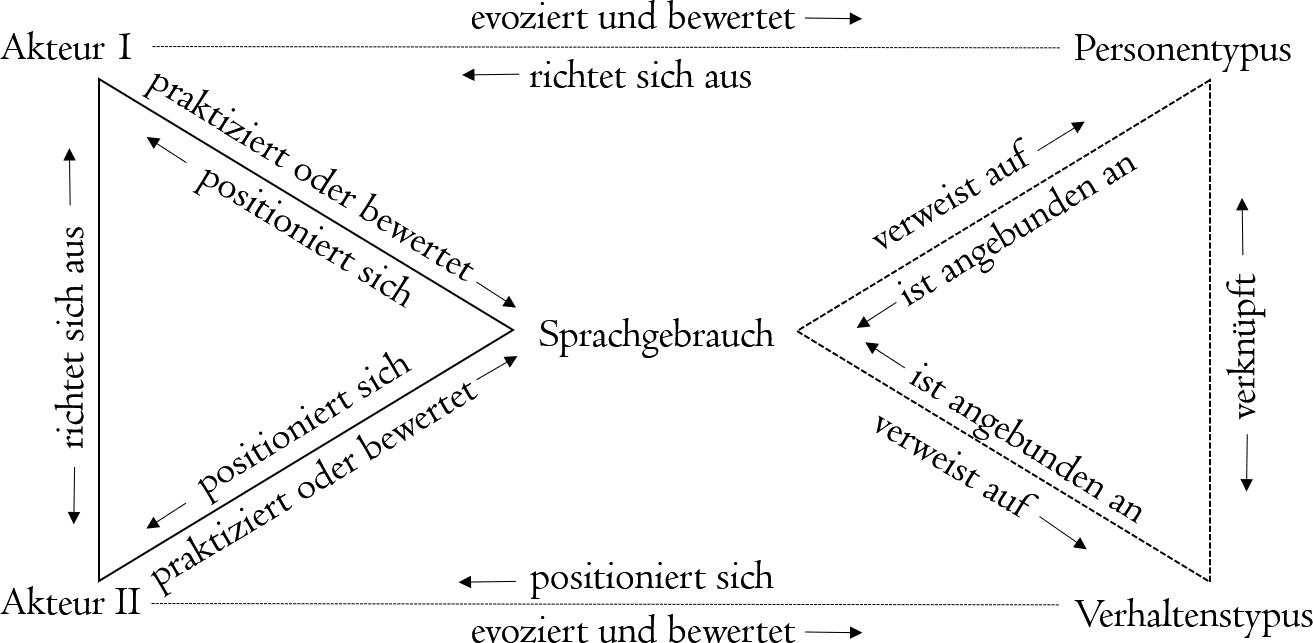
\includegraphics[width=\textwidth]{Briefumschlag}
\caption{Modell der sprachideologischen Positionierung von \citet[273]{Spitzmuller2013}, aktualisiert durch \citeauthor{Spitzmuller2013} (persönliches Gespräch)}
\label{pic:Briefumschlag}
\end{figure}

Wichtig ist jedoch, dass eine Position nicht als etwas anzusehen ist, das im Bewusstsein von Personen verankert ist, sondern als eine Größe, die erst durch eine konkrete Äußerung entsteht~\citep[s.][369--370]{Deppermann.2015}. 
Welche Position jemand relevant macht, kann daher je nach Situation variieren: 
\begin{quote}Positions are locally occasioned and designed, they are temporally and situationally flexible, and they are multifaceted – that is, different facets of identity are relevant in different discursive contexts. \citep[370]{Deppermann.2015}\end{quote}
So lassen sich auch die Rollen von Laie und Expertin als Positionen auffassen, die in einer konkreten Situation eingenommen werden, wie in \autoref{sec:Laienlinguistik} beschrieben. Die Positionierung als Expertin kann dabei etwa durch die Verwendung von Fachbegriffen vorgenommen werden, die als Laie bspw. durch den Ausdruck der emotionalen Bewertung eines Phänomens. 

Mit jeder Verwendung oder metapragmatischen Thematisierung einer indexikalisch aufgeladenen Form sagt eine Person A auch etwas über ihre Ausrichtung gegenüber anderen aus. 
Erstens gegenüber konkreten anderen an der Interaktion beteiligten Personen, etwa wenn eine Person B auf ironische Weise das Wort \object{Personenvereinzelungsanlage} verwendet und Person A darüber lacht. 
Zweitens richtet sie sich dadurch gegenüber einer stereotypen Vorstellung von Personen aus, mit deren Sprachgebrauch dieses Wort assoziiert ist \citep[s.][119]{Gal.2016}. 
Sie positioniert sich also zu einem abstrakten Personentypus, der \citeauthor{Bachtin.1990}s (\citeyear{Bachtin.1990}) Konzept der \textit{Persona} entspricht. 
\textit{Personae} können indexikalisch mit sprachlichen Repertoires verbunden sein, sodass auf sie verwiesen werden kann, indem ein Element dieses Repertoires genutzt wird \citep[s.][118]{Gal.2016}. \citet[39]
{Agha2005} spricht daher von \glqq figures performed through speech\grqq{} und verknüpft die Positionierungstheorie so mit einem zweiten Konzept \citeauthor{Bachtin.1990}s (\citeyear{Bachtin.1990}), dem \textit{voicing}. Damit ist gemeint, dass durch die Verwendung registrierter Formen stereotype Personentypen dargestellt werden können: \glqq every register has a social range, a range of figures performable through its use\grqq{} \citep[39]{Agha2005}. 

Das \textit{voicing}\footnote{In der Soziolinguistik ist oft auch von Stilisierung die Rede \citep[s. bspw.][]{Coupland.2007}.} ist insbesondere durch sprachliche Zeichen dritter oder drei +$n$ter indexikalischer Ordnung(en) möglich. 
Das oben herangezogene Beispiel der Verwendung von \object{ich} mit Aussprache des [\c{c}] als [ʃ] etwa wäre ein Fall von \textit{voicing}, mit dem sich eine Sprecherin oder ein Sprecher gegenüber durch diese Form indizierten Gruppen positionieren kann. 
Dass Indexikalität und Register dynamische Größen sind, die durch die Positionierungspraxis selbst gefestigt, verändert oder infrage gestellt werden können, ist im Positionierungsmodell durch die unterbrochenen Linien dargestellt \citep[s.][273]{Spitzmuller2013}. 
Eine Positionierung zu einer sprachlichen Form ist also nur vor dem Hintergrund der indexikalischen Bedeutung dieser Form zu verstehen und trägt gleichzeitig zur Indexikalisierung der Form bei. 
Ebenso kann sie Anzeichen und Katalysator für Ausblendung, fraktale Rekursivität und Ikonisierung sein. 

\subsection{Spracheinstellungen und Sprachideologien: Theoretische und methodologische Zusammenführung}
\label{sec:Integrationsversuch}
\begin{sloppypar}
Häufig wird von Sprachideologieforschung und Spracheinstellungsforschung als verschiedenen Sichtweisen auf ein und dasselbe Phänomen gesprochen, da beide metapragmatische Bewertungen von Sprache zum Gegenstand haben. 
Bei näherer Betrachtung zeigt sich jedoch, dass die Ansätze unterschiedliche Schwerpunkte haben. 
Während die Sprachideologieforschung an Zusammenhängen von Sprache und Gesellschaft interessiert ist, fokussiert die Spracheinstellungsforschung auf die kognitive Ebene und die Bewertung sprachlicher Phänomene durch einzelne Personen. 
Ziel der Spracheinstellungsforschung ist es dabei in erster Linie, etwas über Varietäten zu erfahren; 
Ziel der Sprachideologieforschung hingegen ist es, etwas über das gesellschaftliche Zusammenleben zu erfahren, sie hat also ein stärker kulturanthropologisch ausgerichtetes Interesse. 
Die Zusammenhänge zwischen der gesellschaftlichen und der individuellen Ebene sollen im \autoref{sec:GesellschaftundIndividuum} erläutert werden. 
Die Kritik an der sozialpsychologisch geprägten Spracheinstellungsforschung lautet oft, ihre Theorie sei unterkomplex und positivistisch (\citealp[s. etwa][141]{Agheyisi.1970}; s. hierzu auch \citealp{Soukup.2014}). 
Inwiefern sich beide Ansätze dennoch unter einem konstruktivistischen Paradigma vereinen lassen, wird in \autoref{sec:Konstruktivismus} diskutiert. 
Schließlich werden aus den Überlegungen methodologische Implikationen für die Untersuchung metapragmatischer Äußerungen abgeleitet (\autoref{sec:Methodologie}). 
\end{sloppypar}
\subsubsection{Metapragmatik zwischen Gesellschaft und Individuum}
\label{sec:GesellschaftundIndividuum}
%Was ist eigentlich mit diesem Gegensatz, dass die Spracheinstellungsforschung verallgemeinern will und die Sprachideologieforschung lokale Praxen untersucht? Muss das noch irgendwo rein? 
Die Begriffe Spracheinstellungen und Sprachideologien können mit \citet[22]{Konig.2014} unterschiedlichen konzeptuellen Ebenen zugeordnet werden. 
Während es bei der Untersuchung von Sprachideologien um Vorstellungen verschiedener sozialer Gruppen geht, stehen bei der Beschäftigung mit Spracheinstellungen die Vorstellungen einzelner Personen im Vordergrund \citep[s.][24]{Konig.2014}.
Zudem werden unter Sprachideologien h{\"a}ufig nicht nur metapragmatische Annahmen zu einzelnen Ph{\"a}nomenen verstanden, sondern Systeme von Vorstellungen {\"u}ber Sprache (\citealp[24]{Konig.2014} verweist hier auf \citealp[970]{Gal.1995} und \citealp[35]{Irvine2000}).

Eine Spracheinstellungsforschung, die aus metapragmatischen Äußerungen kognitive Strukturen ableiten will, verfolgt ein grundsätzlich anderes Ziel als die Sprachideologieforschung, die in Metapragmatik in erster Linie soziale Handlungen sieht.
Vertreter:innen beider Forschungsrichtungen betonen aber den engen Bezug zwischen Sprachideologien und Spracheinstellungen. \citeauthor{Woolard1994} (\citeyear[61--62]{Woolard1994}) sehen in Spracheinstellungen einzelner Sprecher:innen die Spiegelung der in einer Gesellschaft vorhandenen Sprachideologien \citep[vgl. auch][161--162]{Milroy2004}. 
Ähnlich geht \citet[xxiv]{Preston.1999b} davon aus, dass Spracheinstellungen von \textit{folk beliefs} beeinflusst werden, bspw. von Vorstellungen {\"u}ber den Status von Variet{\"a}ten oder über Eigenschaften von deren Sprecher:innen \citep[ähnlich auch][34]{Garrett.2012}.  
Auf solche in der Gesellschaft geteilten, nicht hinterfragten Sprachideologien berufen sich Sprecher:innen bei metapragmatischen Äußerungen (\cites[s.][1]{Gunthner.2012}[vgl. auch][205]{Konig2015}). 
Was die Frage nach der Entwicklung von Spracheinstellungen angeht, h{\"a}lt \citet[732]{Neuland.1993} fest, dass bisherige Untersuchungen hierzu nahelegten, dass Kinder und Jugendliche sich in ihren Spracheinstellungen nach und nach den dominanten Bewertungsmustern der Gesellschaft ann{\"a}herten. 
Auch \citet[399]{Lasagabaster.2005} geht davon aus, dass Sprecher:innen ihre Einstellungen an die in ihrer Gruppe geteilten Ideologien angleichen. 
Dies macht deutlich, wie individuelle Spracheinstellungen von gesellschaftlich geprägten Sprachideologien durchformt werden~\citep[s.][732]{Neuland.1993}. 
Dabei ist davon auszugehen, dass Ideologien alle drei Komponenten speisen, die eine Spracheinstellung konstituieren. 
So besteht etwa die kognitive Komponente im Wesentlichen aus dem Wissen um die Indexikalitäten, die einer Form gesellschaftlich zugeschrieben werden. 
Ebenso lassen sich mit dem Konzept der Indexikalität aber auch die Verhaltensebene (wann verwende ich eine Form/welche Annahmen habe ich darüber, wann ich eine Form verwende?) und die affektive Komponente (mit welchen Emotionen ist eine Form besetzt?) beschreiben. 
Der Bezug der eigenen Einstellung zu gesellschaftlich vermittelten Ideologien ist den Angehörigen einer Sprachgemeinschaft allerdings meist nicht bewusst \citep[s.][133]{Milroy.2007}.

\begin{sloppypar}
Da Sprachideologien von der Gesellschaft reproduziert und dadurch in gewisser Weise normalisiert werden, erscheinen sie als selbstverst{\"a}ndlich~\citep[s.][10]{Blommaert.1999} und können auch Spracheinstellungen wie selbstverst{\"a}ndlich erscheinen lassen \citep[s.][123]{Androutsopoulos.2007}.
Ein Beispiel daf{\"u}r ist der von \citet[134]{Milroy.2007} in Standardsprachkulturen beobachtete {\glqq}belief in correctness{\grqq}:~Auf der Standardsprachideologie, also der Vorstellung einer einheitlichen Leitvariet{\"a}t, fu{\ss}t die Auffassung, manche Varianten seien korrekt und andere inkorrekt. 
Diese Ideologie {\"a}u{\ss}ert sich in einer ablehnenden Einstellung gegenüber manchen Formen, die als {\glqq}falsch{\grqq} eingeordnet und der Folge davon sanktioniert werden~\citep[134]{Milroy.2007}.
\end{sloppypar}

\begin{sloppypar}
Es wird also deutlich, wie eng Spracheinstellungen mit Sprachideologien zusammenhängen: Sprachideologien bestimmen zu einem Teil, wie Sprecher:innen sprachliche Merkmale konzeptualisieren und wie sie sie bewerten \citep[s.][206]{Maitz2015}. 
\citet[8]{Garrett.2012} sieht Sprachideologien daher als Rechtfertigungen und Unterst{\"u}tzungen f{\"u}r Spracheinstellungen. 
Spracheinstellungsäußerungen präsupponieren häufig Sprachideologien, indem sie auf \glqq vorgeformte, soziale Kategorisierungen\grqq{} \citep[][213]{Tophinke.2006} verweisen.
Auf diese Weise lassen Äußerungen über Spracheinstellungen auf zugrundeliegende Sprachideologien schließen \citep[s.][35]{Garrett.2012}.
Sprachideologien und Spracheinstellungen können somit als interdependent modelliert werden:
Vor der Folie etablierter Sprachideologien wie etwa der Standardsprachideologie (s. \autoref{sec:MetapragmatikVariationWandel}) werden Spracheinstellungen geäußert. 
Diese stellen nicht nur eine Positionierung zu einem sprachlichen Phänomen dar, etwa zum Kiezdeutschen, sondern auch zu den damit verbundenen Ideologien. 
So kann bspw. eine negative Einstellungsäußerung zum Kiezdeutschen die Ideologie, der Standard stünde über anderen Varietäten, festigen. 
Trotz dieser engen gegenseitigen Abhängigkeit von Spracheinstellungen und Sprachideologien ist davon auszugehen, dass weder Sprachideologien allein aus Spracheinstellungen entstehen noch Spracheinstellungen sich allein aus Ideologien speisen. 
Bspw. ist es möglich, dass jemand eine positive Einstellung gegenüber einem bestimmten Lexem oder einem bestimmten Dialekt hat, weil er es oder ihn mit dem Sprachgebrauch eines ihm nahestehenden Menschen verbindet. 
Es ist jedoch davon auszugehen, dass Spracheinstellungen nicht ohne grundlegende Konzeptualisierungen von Sprache und damit ohne Rückgriff auf Sprachideologien entwickelt und ausgedrückt werden können:
\end{sloppypar}

\begin{quote}Jeder Standpunktbezug kommuniziert, da er die Bewertung eines {\frq}Objekts{\flq} einschlie{\ss}t und somit Werte und Einstellungen zum Ausdruck bringt, Ideologien.~\citep[270]{Spitzmuller2013}\end{quote}
Für die Entstehung von Sprachideologien auf der anderen Seite sind Spracheinstellungsäußerungen allein nicht ausreichend, sie müssen an bestehende Ideologien anknüpfen und gesellschaftlich geteilt werden. 
In der vorliegenden Studie % Änderung Anfang
soll nicht auf Spracheinstellungen als kognitive Größe, sondern auf Spracheinstellungsäußerungen als konkrete Wertungen fokussiert werden, % Änderung Ende 
die vor dem Hintergrund der in einer Gesellschaft diskursiv ausgehandelten Sprachideologien entstehen und auf diese zurückwirken. 
\subsubsection{Konstruktivistischer Ansatz}
\label{sec:Konstruktivismus}
Wie die Ausführungen zu Spracheinstellungsforschung und Sprachideologieforschung gezeigt haben, unterscheiden sich beide Traditionen zum Teil stark in ihren theoretischen Grundannahmen. 
Der Spracheinstellungsforschung ging es lange Zeit vor allem um die Bewertung selbst und ihre kognitive Manifestation.
So spricht etwa \citeauthor{Neuland.1993} von sprachlichen Formen als Identifikationsmerkmalen, die 
\begin{quote} Attributionen von Merkmalen des Alters und Geschlechts, von nationaler und regionaler Herkunft und Sozialstatus sowie von Pers{\"o}nlichkeitseigenschaften ausl{\"o}sen k{\"o}nnen. \citep[730]{Neuland.1993} \end{quote}
Wie diese Verkn{\"u}pfungen zustande kommen, ist allerdings in vielen Spracheinstellungsstudien nicht Teil der Fragestellung, wie \citet[730]{Neuland.1993} selbst anmerkt.\footnote{Die meisten Spracheinstellungsstudien entsprechen daher dem Ansatz der ersten soziolinguistischen Welle, während die Sprachideologieforschung der dritten Welle verpflichtet ist \citep[s.][]{Eckert2012}.}  
Dennoch beobachtet \citet[120]{Garrett.2007} eine Annäherung an die Sprachideologieforschung, da die Spracheinstellungsforschung zunehmend auch daran interessiert sei, soziale Zuschreibungen kritisch zu hinterfragen.

Das Konzept der Sprachideologien ist hingegen grundsätzlich ein {konstruk\-ti\-vis\-tisches}. 
So stellt \citet[25]{Konig.2014} fest, dass die Sprachideologieforschung verstärkt an der Frage nach semiotischen Prozessen bei der Indexikalisierung und Registrierung sprachlicher Zeichen (\autoref{sec:Indexikalitaet}) interessiert ist. 
In der Sprachideologieforschung werden aber nicht nur die Verknüpfungen von sprachlichen und gesellschaftlichen Kategorien als ideologische Konstrukte angesehen, sondern auch die Kategorien selbst: 
\begin{quote}The “language reflects society” account implies that social structures somehow exist before language, which simply “reflects” or “expresses” the more fundamental categories of the social. Arguably however we need a far more complex model that treats language as \textit{part }of the social, interacting with other modes of behaviour and just as important as any of them. \citep[81--82]{Cameron.1990}
\end{quote}
Auch \citet{Irvine.2005} betont, dass sowohl sprachliche als auch soziale Kategorien nicht als gegeben angenommen werden dürfen: 
\begin{quote}By foregrounding ideology I emphasize the need to investigate ideas about language and speakers independently of empirical distributions, and the need to recognize that {\glq}attitudes{\grq} include participants' basic understandings of what the sociolinguistic system consists of, not just emotional dispositions. Moreover, the categories and behaviors toward which one has these attitudes cannot be assumed to have been established independently of anyone's perception of them.~\citep[24]{Irvine.2005}\end{quote}
Dieser zusätzliche Analyseschritt kann und sollte auch für die Spracheinstellungsforschung nutzbar gemacht werden.  
Auch neuere Spracheinstellungsstudien fordern daher stärker konstruktivistisch ausgerichtete Herangehensweisen (\cites[s.][207]{Tophinke.2006}[195]{Liebscher.2009}[61--62]{Cuonz.2014}).
So machen bspw. \citet[213]{Tophinke.2006} deutlich, dass man zwar davon ausgehen könne, dass Personen einen bestimmten Beruf haben usw., es allerdings von den {Kom\-mu\-ni\-kations\-teil\-neh\-merIn\-nen} abhänge, ob dies im Kontext einer Spracheinstellungsäußerung relevant werde. 

In der diskursiven Sozialpsychologie wird daher ein konstruktivistischer Ansatz verfolgt, der nicht an Einstellungen als mentalen Konstrukten interessiert ist, sondern danach fragt, welche konkreten Bewertungspraktiken sich beobachten lassen und wie Bewertungen von Sprache in der Interaktion genutzt werden (\citealp[s.][234]{Potter.1998}; s. auch die Beiträge in \citealp{Cuonz.2014b}). 
Damit geht eine Verschiebung des Forschungsinteresses einher: 
\begin{quote}Im Sinne des Konstruktivismus ist dabei das Ziel nicht die Suche nach \glqq wahren\grqq{} Spracheinstellungen, sondern die Analyse der Aushandlung von Spracheinstellungen, die immer vor dem Hintergrund von Sprachideologien und Wissen erfolgt.~\citep[109]{Liebscher.2014}\footnote{Was \citet{Liebscher.2014} unter Wissen verstehen, wird hier zu Sprachideologien gezählt.} \end{quote} 
Hier stehen also weniger die Spracheinstellungen selbst als vielmehr Spracheinstellungsäußerungen im Vordergrund.\footnote{\citet[146--149]{Soukup.2014} stellt ausführlich dar, wie sich der Zusammenhang dieser beiden Ebenen in einem grundsätzlich konstruktivistischen Ansatz theoretisch fassen lässt.} 
In dieser Hinwendung der Spracheinstellungsforschung zu interaktionalen Ansätzen wird die Nähe  zum Konzept der sozialen Positionierung deutlich. 
\citet{DuBois.2007} betont zwar, dass die soziale Positionierung nicht mit der kognitiven Manifestation von Einstellungen gleichzusetzen ist: 
\begin{quote}Stance is not something you have, not a property of interior psyche, but something you do -- something you take. Taking a stance cannot be reduced to a matter of private opinion or attitude.~\citep[171]{DuBois.2007}\end{quote}
Konkrete Äußerungen solcher Spracheinstellungen können jedoch durchaus als Positionierung gefasst werden \citep[s.][109]{Liebscher.2014}.\footnote{Ganz ähnlich wie in der Spracheinstellungsforschung wird auch bei der Positionierung unterschieden zwischen \textit{affective }und \textit{epistemic stance} \citep[s. etwa][410]{Ochs1996}. \textit{Affective stance} beinhaltet emotionale Einstellungen und Wertungen, \textit{epistemic stance} hingegen Wissen oder Meinung gegen{\"u}ber einer Sache.}
Als metapragmatische Aussagen stellen sie Positionierungen zur Gesellschaft und ihren Werten dar \citep[s.][258]{Spitzmuller.2005}.
\citet[401]{Lasagabaster.2005} nennt daher \glqq orientating the individual in the social world\grqq{} als eine Funktion, die % Änderung Anfang
Spracheinstellungsäußerungen % Änderung Ende
erfüllen \citep[ähnlich auch][206]{Tophinke.2006}. 

Solche lokalen Positionierungspraxen, wie sie Spracheinstellungsäußerungen darstellen, haben das Potenzial, zu geteilten Sprachideologien zu werden, bspw. indem sie zur Indexikalisierung einer Form beitragen oder die Ausblendung bestimmter sprachlicher Aspekte fördern (\cites[s.][211]{Tophinke.2006}[59]{Cuonz.2014}[8]{Spitzmuller.2017b}).\footnote{Dafür, ob dies geschieht, ist wahrscheinlich nicht unwesentlich, ob eine geäußerte Einstellung auf Zustimmung trifft \citep[s.][211]{Tophinke.2006}.}
Ein konstruktivistischer Ansatz der Spracheinstellungsforschung geht daher davon aus, dass Spracheinstellungsäu{\ss}erungen Wirklichkeit konstruieren. 
\citet[]{Tophinke.2006} verdeutlichen dies an einem Beispiel: 
\begin{quote} Wenn etwa eine bestimmte Varietät Gesprächsgegenstand ist und jemand diese Varietät als \textit{schön} beschreibt, so wird damit nicht nur eine Einstellung geäußert, sondern auch ein bestimmtest Bild dieser Varietät entworfen. \citep[209--210]{Tophinke.2006}\end{quote}
Daneben bringen Spracheinstellungsäußerungen auch stereotype Bilder sozialer Gruppen hervor und tragen so zur sozialen Differenzierung bei. 
Solchen Stereotypen räumen sowohl Spracheinstellungs- als auch Sprachideologieforschung eine wichtige Rolle ein. 
Während in der Spracheinstellungsforschung von Stereotypen gesprochen wird, gibt es in der Sprachideologieforschung das auf \citet{Bachtin.1990} zurückgehende Konzept der \textit{Persona} (s. \autoref{sec:Positionierung}).

Aus den hier dargestellten konstruktivistischen Annahmen und den in \autoref{sec:GesellschaftundIndividuum} beschriebenen Zusammenhängen zwischen Spracheinstellungen und Sprachideologien resultieren einige methodologische Implikationen, die im folgenden Abschnitt besprochen werden sollen. 
Zum Zusammenhang der Begriffe Sprachideologien, Metapragmatik und Spracheinstellungen lässt sich bis hierhin sagen: Alle metapragmatischen Äußerungen werden unter Rückgriff auf in einer Gesellschaft bestehende Sprachideologien getätigt. 
Spracheinstellungsäußerungen bilden eine Teilmenge solcher metapragmatischen Äußerungen, die aus wertenden Positionierungen besteht. 
Jede metapragmatische Äußerung und damit auch jede Spracheinstellungsäußerung wirkt mit an der Tradierung und Weiterentwicklung der bestehenden Sprachideologien.
\subsubsection{Methodologische Implikationen}
\label{sec:Methodologie}
Was die Methodologie angeht, überschneiden sich Sprachideologie- und Spracheinstellungsforschung deutlich und bedienen sich beide an den in der jeweils anderen Tradition gebräuchlichen Herangehensweisen. 
So hält \citet{Garrett.2012} fest, die Sprachideologieforschung sei nicht auf eine bestimmte Methodologie festgelegt, und sieht in der Verwendung von Methoden der Spracheinstellungsforschung eine mögliche Herangehensweise auch für sprachideologische Fragestellungen: 
\begin{quote}Research into language ideologies is not linked to any specific methodological tradition, although critical discourse analytical procedures constitute one approach within sociolinguistics. Language attitudes research can arguably be seen, though, as one set of methodological options for studying language ideologies.~\citep[35]{Garrett.2012}\end{quote}
Insgesamt lässt sich aber sagen, dass die Sprachideologieforschung vorwiegend mit ethnografischen Methoden wie bspw. Gruppeninterviews arbeitet, während die Spracheinstellungsforschung über ein recht ausdifferenziertes Set an überwiegend {so\-zial\-psycho\-lo\-gisch} geprägten Methoden verfügt. 
Allerdings wäre es aufgrund des engen Zusammenhangs von Ideologien und Einstellungen wünschenswert, dass die gewählte Methode den Einbezug beider Konzepte gewährleistet \citep[s.][196]{Liebscher.2009}.

Für die konkrete Wahl der Methode sind verschiedene Faktoren relevant, auf die im Folgenden eingegangen wird.
\citet[64]{Adler.2018} machen deutlich, dass man sich bei der Entscheidung für eine Methode auf einem Kontinuum bewegt zwischen der Erhebung vieler, nicht allzu komplexer und daher leicht auszuwertender Daten und der Erhebung weniger komplexer Daten. 
Zudem ist ausschlaggebend, inwiefern von den Daten allgemeingültigere Aussagen abgeleitet werden sollen und ob bspw. verschiedene soziale Gruppen zu berücksichtigen sind \citep[s.][64]{Adler.2018}. 
Sinnvoll ist aber insbesondere auch eine Kombination verschiedener Erhebungs- und Datentypen \citep[s.][144--145]{Soukup.2014}.

%Perzept und Konzept
Relevant ist außerdem \citeauthor{Preston2010b}s (\citeyear{Preston2010b}) Unterscheidung zwischen Perzept und Konzept: Werden Perzepte untersucht, geht es darum, wie Sprecher:innen pr{\"a}sentierte Beispiele wahrnehmen~\citep[1--2]{Preston2010b}. 
Bei der Erhebung von Konzepten hingegen stehen die Vorstellungen, die Sprecher:innen von etwas haben, im Vordergrund \citep[1]{Preston2010b}. 
Die Frage \textit{welche Phänomene mögen Sie im Deutschen?} wäre also eine Frage nach einem Konzept, während die Frage \textit{wie finden Sie die Form g\,e\,w\,i\,n\,k\,t?} nach dem Perzept fragt. 
\citet[2--3]{Preston2010b} weist jedoch darauf hin, dass Konzept und Perzept kaum strikt voneinander separierbar seien.

%Manifestation
Dafür, welche Methoden infrage kommen, ist auch entscheidend, woran sich nach Ansicht der Forschenden Sprachideologien bzw. Spracheinstellungen ablesen lassen. 
Prinzipiell kann praktisch jede Art von verbaler oder nonverbaler metapragmatischer Handlung, in der eine Sprach\-ein\-stel\-lung zum Ausdruck kommt, für die Untersuchung der Einstellung genutzt werden \citep[s.][242]{Ajzen1989}. 
\citet[1320--1321]{Vandermeeren2005} unterscheidet hier die Beobachtung tatsächlichen Sprachgebrauchs, der Sprach\-ein\-stel\-lungen reflektieren kann, und die Beschäftigung mit Aussagen über den eigenen Sprachgebrauch oder über Spracheinstellungen und weist darauf hin, dass es hier zu Widersprüchen kommen kann. 
In der Sprachideologieforschung gibt es unterschiedliche Ansichten darüber, wie sich Sprachideologien konkret äußern:~W{\"a}hrend einige explizite {\"A}u{\ss}erungen als Evidenz voraussetzen (bspw. \citealp{Silverstein1979}, wie seine Definition als \glqq articulated beliefs\grqq{} deutlich macht), sehen andere auch in gesellschaftlichen Strukturen und unbewusstem Handeln Repr{\"a}sentationen von Sprachideologien~\citep[s.][57--58]{Woolard1994}. 
Von \citet[52]{Irvine1998} und \citet[43]{Silverstein.1976} wird jedoch betont, dass der tatsächliche Sprachgebrauch klar von dem unterschieden werden muss, was Sprecher:innen {\"u}ber Sprache und sprachliche Formen annehmen. 
%Dies zeigt sich oft an der Diskrepanz zwischen beidem: So lehnen bspw. viele Sprachbenutzer:innen \object{weil} mit Verbzweitstellung als falsch ab und geben an, es selbst nicht zu verwenden, obwohl es sich in ihrem Sprachgebrauch durchaus findet \citep[][]{Beleg???}.

%Drei Ansätze
\citeauthor{Garrett2005} (\citeyear{Garrett2005}, s. auch  \citealp[37]{Garrett.2012}) unterscheidet bei der Erhebung von Sprach\-ur\-tei\-len drei Ans{\"a}tze, die sich voneinander unterscheiden lassen:~\textit{societal treatment}, \textit{indirect approach} und \textit{direct approach}.\footnote{Auch \citet[212--213]{Cargile.1994} stellen diese drei verschiedenen methodischen Ans{\"a}tze vor, die sie inhaltsanalytisch, direkt und indirekt nennen.} 
Mit \textit{societal treatment} sind etwa Diskursuntersuchungen gemeint, die % Änderung Anfang
Spracheinstellungsäußerungen % Änderung Ende
zum Thema haben. 
Ein solcher Ansatz hat vor allem den Vorteil, dass er wenig eingreifend ist \citep[s.][52]{Garrett.2012}. 
Direkte Ans{\"a}tze fragen Proband:innen offen nach ihrer Einstellung. 
Indirekte Ans{\"a}tze versuchen, an die Einstellungen heranzukommen, ohne direkt zu fragen~\citep[s.][]{Garrett2005}.\footnote{Davon, dass sich mit dem direkten Ansatz nur bewusste Konzeptualisierungen und mit dem indirekten Ansatz nur unbewusste erfassen lie{\ss}en, kann wahrscheinlich nicht ausgegangen werden. 
Bei der Bewertung spielen immer sowohl bewusste als auch unbewusste Prozesse eine Rolle~\citep[s.][4--5]{Preston2010b}. 
\citet[178--179]{Studler.2014} nimmt aber an, der indirekte Ansatz k{\"o}nne lediglich unbewusste Einstellungen erfassen und sei daher unzul{\"a}nglich, w{\"a}hrend der direkte Ansatz sowohl unbewusste als auch bewusste Einstellungen erfasse.}
%Matched-Guise
Ein typischer indirekter Ansatz ist die von \citet{Lambert.1960} entwickelte Matched-Guise-Technik. Bei dieser Methode werden Proband:innen gebeten, Sprachproben vermeintlich verschiedener Sprecher:innen zu bewerten. Tatsächlich bekommen sie aber Sprachproben ein und derselben Person in verschiedenen Varianten -- bspw. in verschiedenen Dialekten -- zu hören. So wird ausgeschlossen, dass unbewusst etwa Eigenschaften der Stimme bewertet werden, und sichergestellt, dass Unterschiede in der Bewertung auf die verschiedenen Stile zurückzuführen sind. 

Der direkte und der indirekte Ansatz sind auf Erhebungen durch Fragebögen oder Interviews angewiesen. 
Ob dafür eine schriftliche oder eine mündliche Befragung vorgenommen wird, hat einen Einfluss auf die erhobenen Daten. 
Ein mündliches Interview bringt mehr Interaktion zwischen Befragten und Befragenden mit sich, was bspw. Rückfragen ermöglicht \citep[s.][1255]{Garrett2005}. 
Die interviewende Person hat dadurch einen größeren Anteil an der kollaborativen Konstruktion von metapragmatischen Urteilen in der Interviewsituation. 
Mit schriftlichen Befragungen lassen sich allerdings sehr viel mehr Personen erreichen. 
Da die Antworten nicht transkribiert werden müssen, ist es auch leichter möglich, eine größere Menge an Daten zu bearbeiten. 

%offene und geschlossene Fragen
Typischerweise enthalten Fragebögen geschlossene Fragen \citep[s.][181]{Studler.2014}.
Diese geben Antwortmöglichkeiten vor, sodass die Befragten lediglich eine oder mehrere dieser Möglichkeiten auswählen können \citep[s.][55]{Porst2014}.
Der Vorteil besteht in der relativ unkomplizierten Auswertung und darin, dass sich die Antworten gut vergleichen lassen, bspw. auch bei skalierten Antworten (etwa Stufen zwischen \textit{sehr schön} und \textit{gar nicht schön}) (\cites[s.][215]{Garrett.2004}[74]{Adler.2018}). 

%Matched-Guise und Semantische Differenziale
Zu Methoden, die mit geschlossenen Fragen arbeiten, lassen sich etwa semantische Differenziale zählen, die häufig als Messinstrument bei der Matched-Guise-Technik eingesetzt werden \citep[s.][13]{Hundt.1992}.
Mit einem solchen Vorgehen können jedoch nur die Konzeptualisierungen und indexikalischen Bedeutungen abgefragt werden, von denen man bereits bei der Erstellung der Frage wusste \citep[s.][196]{Garrett.2004}. 
Daraus ergeben sich im Wesentlichen zwei Probleme: Erstens erfährt man nichts über mögliche weitere indexikalische Bedeutungen. 
Zweitens verzerrt eine solche Art der Frage unter Umständen die Relevanz der abgefragten Kategorien.  
Bittet man Proband:innen bspw. um ein Kreuz auf einer Skala, bewerten sie die Variet{\"a}t oder Variante auch bereitwillig in Kategorien, die ihnen bei freien Assoziationen nicht einfallen würden.  
Zudem kann bereits die Reihenfolge der präsentierten Auswahlmöglichkeiten einen Einfluss auf die Antworten haben \citep[s.][138]{Porst2014}. 
Sowohl die Kategorien selbst als auch deren Reihenfolge müssen daher sehr sorgfältig gewählt und gut begründet werden \citep[s.][70]{Adler.2018}.
Inwiefern sich metapragmatische Urteile allein durch geschlossene Fragen erheben lassen ist unter diesen Voraussetzungen fraglich.
\citet[216]{Garrett.2004} etwa sehen es als unmöglich an, Bewertungsdaten mithilfe eines vorgegebenen Antwortsets erschöpfend zu erheben. 
Offene Fragen hingegen lassen die Teilnehmer:innen ihre Antworten selbst formulieren. 
Da sie sehr viel aufwändiger auszuwerten sind und daher als anspruchsvoller angesehen werden, kommen offene Fragen seltener zum Einsatz \citep[s.][70--71]{Adler.2018}. 
Sie sind jedoch die einzige Möglichkeit, etwas über die Konzeptualisierung der Befragten selbst zu erfahren, denn
\begin{quote}während mit einem geschlossenen Format, dessen Antwortoptionen ein Feld inhaltlich abzudecken scheinen, tatsächlich Verzerrungen entstehen können, eben weil die Antwortoptionen doch nicht exhaustiv sind, ermöglicht es das offene Format, gerade weil keine Antwortoptionen vorgegeben sind und die Antworten typischerweise sehr heterogen ausfallen, bestimmte laienlinguistische Konzeptualisierungen und unerwartete Bezugssysteme aufzudecken, die sonst nicht oder nur wenig bekannt sind. \citep[71]{Adler.2018}\end{quote}
Freie Antworten können daher als valider und aussagekräftiger gelten, auch weil sie im Gegensatz zu geschlossenen Fragen Begründungen liefern können \citep[s.][182--183]{Studler.2014}.
Allerdings müssen offene Fragen sehr fokussiert formuliert sein, damit es bei der Auswertung nicht eine zu große Menge Antwortkategorien gibt~\citep[s.][62--63]{Porst2014}.
Ansonsten wird eine anschließende Inhaltsanalyse, bei der die Antworten zu Kategorien und Oberkategorien zusammengefasst werden sollen, deutlich erschwert \citep[s.][3]{Schreier.2014}. 

\citet[196]{Garrett.2004} plädieren für die stärkere Nutzung von offenen Fragen nach Bewertungen, die häufig nur als Vorstudie für die Auswahl der Items von semantischen Differnzialen dienen. 
Dafür spreche schon, dass solche Items allein durch die Anforderung, skalierbare, antonymfähige Adjektive sein zu müssen, sehr eingeschränkt seien \citep[s.][196]{Garrett.2004}. 
Sie sehen die Frage nach freien Assoziationen als gute M{\"o}glichkeit, Sprachurteile zu erheben, v.\,a. da sie den Facettenreichtum der Ideologien und Einstellungen zeigen~\citep[s.][215]{Garrett.2004}. 
In einer Studie zu Einstellungen zu walisischen Dialekten unter Jugendlichen stellen sie daher die offene Frage \glqq [w]rite down your first impressions when you listen to the speaker\grqq{} \citep[201]{Garrett.2004}.
Erst im Anschluss werden geschlossene Fragen gestellt \citep[s.][201]{Garrett.2004}. 
Insgesamt sehen \citeauthor{Garrett.2004} große Vorteile in dieser Erhebungsweise. 
Die erhobenen Assoziationen
\begin{quote}offer a shorthand for evaluative discourses, and how they are structured within particular groups. We see how evaluative language does more than hang qualities or attributes on targets. \citep[216]{Garrett.2004}\end{quote}
In den Antworten auf die offene Frage zeigt sich bspw. teilweise eine starke Emotionalität, die durch die schlichte Erhebung über Skalen verdeckt bliebe \citep[s.][216]{Garrett.2004}.
Diese Art von freien Antworten erlaubt also nicht nur eine inhaltsanalytische Auswertung, sondern lässt zusätzlich die Positionierung von Befragten zu geäußerten Sprachideologien erkennen (\cites[s.][119]{Liebscher.2014}[170]{Studler.2014}). 
Eine Möglichkeit, diese zu untersuchen, ist etwa die Analyse von Präsuppositionen, also dem, was mit einer sprachbewertenden Äußerung implizit vorausgesetzt wird \citep[s.][199]{Liebscher.2009}. 
So können bspw. epistemische Marker wie \object{ich finde} oder \textit{natürlich} darauf hinweisen, ob eine % Änderung Anfang
geäußerte % Änderung Ende
Bewertung als in der Sprachgemeinschaft geteiltes Wissen oder als persönliche Einschätzung angesehen wird \citep[s.][376]{Deppermann.2015}. 

Auf diese Weise lässt sich die direkte Erhebung metapragmatischer Urteile verbinden mit einem indirekten Ansatz, der auch die Positionierung in den Blick nimmt \citep[s.][110]{Liebscher.2014}. 
Dies macht deutlich, was auch \citet[145]{Soukup.2014} betont:
Keineswegs sind der direkte und der indirekte Ansatz nur für Forschungsfragen in einem positivistischen Paradigma geeignet, sondern auch für konstruktivistische Fragestellungen lassen sie sich sehr gut nutzen. 

%einzelne Varianten
Entscheidend für die Wahl des konkreten Ansatzes sollte nicht zuletzt sein, welches sprachliche Phänomen in den Blick genommen wird. 
Insbesondere im Bereich der Spracheinstellungsforschung gibt es bisher kaum Untersuchungen zu einzelnen Varianten, sondern die Studien (etwa die des Instituts für Deutsche Sprache, \citealp[s.][]{Adler.2018}) beziehen sich beinahe immer auf ganze Dialekte, Regionalsprachen, Fremdsprachen usw.~(\citealp[s.][1251]{Garrett2005}; s. zu grammatischen Varianten im Englischen aber etwa \citealp{Ebner.2018}).
\citet[39--40]{Preston2004} weist jedoch darauf hin, dass es notwendig ist, den Einfluss einzelner Features auf die Einstellung von Lai:innen zu untersuchen und hebt hervor, dass dies bisher zu wenig gemacht wurde. 
Er schl{\"a}gt vor, {\"a}hnliche Tests auch f{\"u}r andere Features durchzuf{\"u}hren. Bspw. fragen \citet{AlBanyan.1998} Studierende, in welcher Situation sie die hyperkorrekte Variante  \textit{the award was given to Bill and I }verwenden w{\"u}rden. 
Die Ergebnisse dieser Studie zeigen unter anderem, dass auch einzelne Features mit Spracheinstellungen verbunden sein k{\"o}nnen \citep[s.][44]{Preston2004}.

Eine m{\"o}gliche Vorgehensweise bei der Untersuchung einzelner Varianten sieht \citet[1693]{Preston2005} in der Pr{\"a}sentation von Beispielen und der Bewertung dieser durch Befragte.
Eine sprachliche Form f{\"u}hrt nicht unmittelbar zu einer Reaktion bei H{\"o}rer oder Leserin. 
Der Reaktion sind vielmehr nicht nur die Einstellungen vorausgeschaltet, sondern auch ein Auswahlprozess von Seiten des H{\"o}rers/der Leserin, in dem sich entscheidet, welche Merkmale {\"u}berhaupt die Bewertungsgrundlage bilden \citep[s.][218]{Cargile.1994}. 
Um Einstellungen zu konkreten grammatischen Varianten zu erheben, ist ein Fragebogen, der diese Variante gezielt pr{\"a}sentiert, daher ein sinnvolles Instrument~\citep[s.][218]{Cargile.1994}. 
Der direkte Ansatz erlaube die gezielte Untersuchung von % Änderung Anfang
Einstellungsäußerungen % Änderung Ende 
gegen{\"u}ber vorab definierten, auch kleinteiligen Variationsph{\"a}nomenen wie grammatischer Variation und bringe damit einige Vorteile mit sich, so \citet[213]{Cargile.1994}.

Dabei muss stets abgewogen werden zwischen geringer Kontrollierbarkeit der Variablen und K{\"u}nstlichkeit der Situation~\citep[s.][4]{Hundt.1992}. 
\citet[1254]{Garrett2005} beschreibt etwa das Vorgehen, mit sogenannten Vignetten zu arbeiten: 
Dabei werden den Proband:innen kurze Szenarien präsentiert, innerhalb derer eine sprachliche Form bewertet werden soll. 
Das Arbeiten mit solchen Szenarien oder Vignetten hat den Vorteil, dass die Befragten ein Phänomen vor einem bestimmten Kontexthintergrund und nicht völlig isoliert beurteilen. 
Allerdings gibt \citet[1254]{Garrett2005} zu bedenken, dass es sich dennoch um konstruierte Bewertungssituationen handelt, die sich von natürlichen Alltagssituationen stark unterscheiden. 
Wird dies bei der Auswertung entsprechend berücksichtigt, gibt es jedoch keinen Grund, in diesem Kontext geäußerte Sprachurteile nicht als valide Daten zu interpretieren \citep[s.][146]{Soukup.2014}.

%Befragungskontext
Unabhängig davon, welche konkrete Methode gewählt wird, muss immer mitberücksichtigt werden, dass die ge{\"a}u{\ss}erten Sprachideologien und Spracheinstellungen eine Positionierung auch zur Interviewerin sind~\citep[s.][133]{Gal.2016}.\footnote{Andersherum ist es natürlich ebenso relevant, die eigene Position(ierung) als Forscher:in mitzubedenken \citep[s.][13]{Spitzmuller.2017b}.} 
Insbesondere Antworten auf offene Fragen, aber auch die Auswahl von Antwortmöglichkeiten lassen sich als diskursive Einstellungsäußerung in der Interaktion mit dem Fragebogen bzw. der dahinterstehenden Institution oder der Forscherin sehen \citep[s.][71]{Adler.2018}. 
Es lassen sich daher 
\begin{quote} auch quantitative SprecherInnen-Evaluierungsexperimente als eine Form von Interaktion [...] betrachten, und zwar eben als eine solche, in der die Einstellungskonstruktion eine zentrale Rolle einnimmt. \citep[145]{Soukup.2014}\end{quote} 
Kontextfaktoren einer Befragung sind somit als sehr relevant zu beurteilen und müssen bei der Analyse berücksichtigt werden \citep[s.][46]{Garrett.2012}. 
So werden etwa die Elemente eines Fragebogens oder die Varietät, in der die Fragen gestellt werden, von den Befragten als Kontextualisierungshinweise gedeutet und können die gegebenen Antworten beeinflussen \citep[s.][144]{Riehl.2000}. 
Auch der institutionelle Rahmen, in dem eine Befragung stattfindet, muss bei der Interpretation der Antworten berücksichtigt werden \citep[s.][14]{Konig.2014}. 
\citeauthor{Vandermeeren1996} (\citeyear[159]{Vandermeeren1996}; s. auch \citeyear{Vandermeeren2005}) erweitert das klassische Drei-Komponenten-Modell daher um Parameter, die die Äußerung einer Spracheinstellung beeinflussen, wobei sie den Kontext und die Gegebenheiten einer Befragung berücksichtigt. 
Bspw. ist mit \citet[208--209]{Tophinke.2006} davon auszugehen, dass Personen ihre Einstellungsäußerung an geforderte Normen anpassen. 
D.\,h., wenn jemand \glqq die normativen Erwartungen in einer Situation als besonders verbindlich [einschätzt], wird seine Einstellungsäußerung diese normativen Erwartungen berücksichtigen\grqq{} \citep[209]{Tophinke.2006}. 
Der Effekt der sozialen Erw{\"u}nschtheit stellt also immer eine Schwierigkeit bei Befragungen zu Einstellungen dar (\cites[s.][182]{Plewnia.2011}[44]{Garrett.2012}).
Möglich ist aber auch, dass Normerwartungen bewusst verletzt werden, um dadurch eine bestimmte Selbstinszenierung vorzunehmen \citep[s.][214--215]{Tophinke.2006}.
Diese besondere Relevanz von durch Sprachideologien vermittelten Normerwartungen muss in die Analyse einbezogen werden. % Änderung Anfang
Auch für die vorliegende Untersuchung gilt, dass die Antworten der Befragten als Positionierungen gegenüber der Forscherin und der Institution Universität gewertet werden müssen. 
Die theoretischen Überlegungen zur sprachideologischen Positionierung sind also bedeutsam für die Auswertung der Befragung. % Änderung Ende

Die Ausführungen zur Methodologie lassen sich in folgenden Leitfragen zusammenfassen, die bei der Studien zu metapragmatischen Urteilen berücksichtigt werden müssen:
\begin{enumerate}
\item Geht es um ein Set sprachlicher Zeichen (Register) oder einzelne Formen?
\item Stehen im Fokus des Interesses Perzepte oder Konzepte? 
\ Sollen die Daten quantitativ oder qualitativ ausgewertet werden? 
\item Soll ein diskurslinguistischer, ein indirekter, ein direkter Ansatz oder eine Kombination daraus gewählt werden? 
\item Wenn eine Befragung stattfindet, soll sie mündlich oder schriftlich stattfinden? 
\item Sollen offene oder geschlossene Fragen gestellt werden? 
\end{enumerate} 
Dabei geht es in den meisten Fällen nicht zwangsläufig um Entweder\hyp oder\hyp Entscheidungen, sondern die verschiedenen Herangehensweisen können sinnvoll kombiniert werden. 
So schlägt etwa \citet[179]{Studler.2014} vor, offene und geschlossene Fragen zu verbinden, um so eine Auswertung nach quantitativen und qualitativen Gesichtspunkten zu ermöglichen. 
Mit einem solchen Vorgehen lasse sich einerseits zeigen, 
\begin{quote}dass eine bestimmte Variable einen prognostizierten Effekt auf eine andere Variable hat -- mittels quantitativer Methode und deskriptiver/inferentieller Statistik; andererseits kann aufgezeigt werden, wie und warum die prognostizierte Beziehung tatsächlich auftritt -- mittels qualitativer Methode und inhaltsanalytischer oder diskursanalytischer Betrachtung. \citep[179]{Studler.2014}\end{quote}
Im folgenden Abschnitt geht es um die Frage, warum die Untersuchung metapragmatischer Urteile für die Erforschung von Sprachvariation und -wandel relevant ist. 

\section[Zusammenhang von Metapragmatik, Sprachvariation und Sprachwandel]{Zum Zusammenhang von Metapragmatik, Sprachvariation und Sprachwandel}
\label{sec:MetapragmatikVariationWandel}
\begin{sloppypar}
In \autoref{sec:Konstruktivismus} war bereits die Rede davon, dass Konzeptualisierungen von Sprache die soziale Wirklichkeit mitformen. 
Sowohl in der Sprachideologieforschung als auch in der Spracheinstellungsforschung geht man aber auch davon aus, dass Bewertungen von und Urteile über Sprache die Sprache selbst beeinflussen k{\"o}nnen~\citep[s.][xxiv]{Preston.1999b}. 
\citet[45]{Preston2004} etwa betont die Relevanz metapragmatischer Urteile für sprachliche Variation.
% Änderung Anfang
Soziale Strukturen wirken sich also mittelbar auf den Sprachgebrauch aus, indem sie metapragmatische Wertungen prägen. 
Diese zentrale Bedeutung gesellschaftlicher Zusammenhänge für die Verwendung sprachlicher Formen wurde in der frühen Sprachvariations- und Sprachwandelforschung kaum berücksichtigt und erst durch Labovs \textit{language variation and change}-Ansatz zu einem Kernthema der modernen Linguistik \citep[s.][25]{Hazen.2011}.
Laut \citet[75]{Labov.2006} sind Variation und Wandel nicht allein mit innersprachlichen Faktoren erklärbar, sondern nur vor dem Hintergrund der sozialen Zusammenhänge in der Sprachgemeinschaft.
% Änderung Ende
\end{sloppypar}

Zwischen Metapragmatik, Variation und Wandel besteht also ein enges Zusammenspiel. 
Dabei stehen sprachliche Variation und das Bewusstsein f{\"u}r diese in engem Zusammenhang mit dem Konzept der Standardsprache sowie mit Normorientierung und Schriftlichkeit \citep[s.][325]{Langer.}. 
In besonderem Maße ist für die Beschäftigung mit grammatischen Varianten daher die Standardsprachideologie relevant, also die Vorstellung von einer einheitlichen Varietät, die über allen anderen Varietäten einer Sprache steht \citep[s.][]{Milroy2001}.
In \autoref{sec:Einheitlichkeit} wird ausgeführt, inwiefern die Vorstellung von der Einheitlichkeit der Standardsprache dazu führt, dass Variation und Wandel häufig negativ wahrgenommen werden.
\autoref{sec:Prestigevarietaet} behandelt anschließend die Registrierung der Standardsprache als Prestigevarietät. 
Schließlich geht es in \autoref{sec:WandeldurchIndexikalitaet} darum, wie metapragmatische Bewertungen und Konzeptualisierungen auf die sprachliche Variation zurückwirken und den Sprachwandel lenken können. 
\subsection{Ideologie der Einheitlichkeit}
\label{sec:Einheitlichkeit}
Die Standardisierung einer Sprache ist ein andauernder Prozess, der nie zu einem Abschluss kommen kann (\cites[s.][22]{Milroy1991}[534]{Milroy2001}). 
Dies liegt unter anderem an der Imperfektibilität des Sprachsystems, die zu diachroner und synchroner Variation führt \citep[s.][]{Antos2003}, aber auch daran, dass regional unterschiedliche Standardvarietäten verwendet werden \citep[s.][]{Ammon.2005}. \citet[29]{Ammon.2005} sieht \glqq die im öffentlichen Sprachgebrauch normalen Sprachformen\grqq{} als Standard und führt aus, dass diese oftmals keine Gültigkeit für das gesamte deutschsprachige Gebiet haben. 
So sei \object{Matura} nur in Österreich % Änderung Anfang
und in der Schweiz % Änderung Ende 
gebräuchlich, \object{Abitur} hingegen nur in Deutschland. 
Die Standardvarietät erreicht also nie den Status vollst{\"a}ndiger Einheitlichkeit -- ihre Uniformit{\"a}t bleibt ein Konstrukt in der Vorstellung der Sprachbenutzer:innen der Standardsprachkultur~\citep[s.][134]{Milroy.2007}. 
\citet[17]{Maitz.2015} spricht von der Ideologie des sprachlichen Platonismus, die in der {\"U}berzeugung besteht, es gebe einen idealen Zustand der Sprache, der von ihrem Gebrauch losgel{\"o}st ist. 
Ähnlich stellt \citet[55]{Preston2004} fest, es existiere die Vorstellung von einer Sprache, die losgelöst sei von jeglichem Gebrauch und \glqq external to human cognitive embedding -- somewhere \glq out there\grq \grqq.\footnote{Aber auch der in der Linguistik lange Zeit propagierte Ansatz \glqq leave your language alone\grqq{} sieht die Sprache, wie \citet[4--5]{Cameron1995} deutlich macht, als von ihren Benutzer:innen losgelöstes Phänomen, das von diesen am besten nicht kommentiert oder gar verändert werden sollte.}

%richtig falsch 
Obwohl die Einheitlichkeit der Sprache also nicht erreicht werden kann, gehen viele Sprecher:innen von einem starren Sprachsystem und einer abgeschlossenen Standardisierung aus, die zu einer vollständigen Vereinheitlichung geführt hat und jeweils genau eine Variante als die richtige festlegt:\footnote{Zur Problematisierung dieser teleologischen Sichtweise in der Sprachgeschichtsforschung s. \cite[]{Elspa2005} \citeyear[]{Elspa.2005} und \citeyear[]{Elspa2005}.}
\begin{quote}In what I have above called standard-language cultures, virtually everyone subscribes to the ideology of the standard language, and one aspect of this is a firm belief in correctness. This belief takes the form that, when there are two or more variants of some word or construction, only one of them can be right. It is taken for granted as common sense that some forms are right and others wrong, and this is so even when there is disagreement as to which is which.~\citep[535]{Milroy2001}\end{quote}
Die Einheitlichkeit der Standardsprache gilt als erstrebenswert, weshalb z.\,B. bei der Sprachpflege Variation m{\"o}glichst unterdr{\"u}ckt werden soll, um die wahrgenommene Regelhaftigkeit der Sprache zu beweisen und zu bewahren~\citep[s.][17]{Woolard1998}. 
Variation wird meist als Unvollkommenheit der Sprache betrachtet (\cites[s.][330]{Langer.}[163]{Gal.2016}). 
\citet[16]{Klein2003} sieht in dieser starken Orientierung an einer einheitlichen Standardsprache die Grundlage dafür, dass Sprecher:innen häufig zweifeln, welche von zwei oder mehr grammatischen Varianten gewählt werden sollte: Da Sprachbenutzer:innen von nur einer korrekten Variante ausgehen, können sie sich die Variation nicht erklären und sind verunsichert.
Dies beobachten auch \citet{Topalovic2008}: 
\begin{quote}
Das beschriebene Nebeneinander zweier Formen führt nicht nur zu Unsicherheiten bei den meisten Sprecher/innen hinsichtlich solcher sprachlicher Normen, es widerspricht offenbar auch einer verbreiteten Ansicht zu \glq korrektem Hochdeutsch\grq: In unserer Gesellschaft ist, wie die öffentlichen Debatten zeigen, die Auffassung besonders ausgeprägt, dass nur eine der beiden Formen die bessere bzw. nur eine \glq richtig\grq{} sein kann.~\citep[41]{Topalovic2008}\footnote{\citet{Topalovic2008}, \citet{Hennig2009} und zahlreiche andere Linguist:innen sehen in dem starken Bedürfnis der Sprachbenutzer:innen nach einer klaren Distinktion zwischen Richtig und Falsch ein Vermittlungsproblem zwischen der Sprachwissenschaft und der Sprachöffentlichkeit.}\end{quote}
Sie machen hier einen Unterschied zwischen Lexik und Grammatik aus: Während etwa regional bedingte lexikalische Variation begrüßt wird, werden \glqq regional oder umgangssprachlich bedingte \textit{grammatische} Varianten mehr oder weniger explizit als Abweichungen von einem \glq Idealdeutsch\grq{} abgewertet\grqq{} \citep[46, Hervorhebung im Original]{Topalovic2008}. 
Auch in Interviews, in denen \citet{Beuge2017} linguistische Lai:innen zu deren Vorstellung von gutem Deutsch befragt, zeigt sich, dass insbesondere diatopische grammatische Variation negativ beurteilt wird.

%Wandel
Aus der Standardsprachideologie resultiert auch der Wunsch nach Unveränderlichkeit des Sprachgebrauchs.
Sprachwandel vollzieht sich in der Regel sehr langsam, sodass Sprachbenutzer:innen den falschen Eindruck bekommen können, das Sprachsystem sei ein statisches Gebilde.
Diese Ideologie führt zu dem Wunsch nach festgelegten, gleichbleibenden Normen.
Unter den Anrufer:innen des Essener Sprachtelefons bspw. beobachten \citet[125]{Bunting1996}, dass diese von der Unveränderbarkeit sprachlicher Normen ausgehen. 
Wandel wird dann oft mit Uneinheitlichkeit und Regellosigkeit gleichgesetzt, sprachliche Neuerungen werden als unzulässige, {sanktions\-be\-dürf\-ti\-ge} Normverstöße empfunden \citep[s.][34]{Hennig2009}. 

Zu einer ähnlichen negativen Beurteilung des Sprachwandels führt die Metapher von Sprache als organischem Körper mit einer Jugend-, Blüte- und Alterungsphase \citep[s.][89--90]{Kilian2010}: Sprachwandel wird hier als Sprachverfall gedeutet und soll daher durch Kritik aufgehalten werden. 
Diese Auffassung gibt es bereits im 17. Jahrhundert in den Sprachgesellschaften \citep[s.][39]{Hundt.2000}. 
Deren Ziel ist es unter anderem, den Sprachwandel anzuhalten oder im besten Falle rückgängig zu machen \citep[s.][41]{Hundt.2000}.
Ähnliche Ansichten vertreten später zahlreiche einflussreiche Autoren wie Grimm und Humboldt, wie \citet[10--11]{Labov.2006} anführt.
Ein Beispiel dafür findet sich in \citet[]{Wustmann.1911}, der zum Gebrauch des Imperfekts schreibt: 
\begin{quote} Ganz widerwärtig und ein trauriges Zeichen der zunehmenden Abstumpfung unsers Sprachgefühls ist ein Mißbrauch des Imperfekts, der seit einiger Zeit mit großer Schnelligkeit um sich gegriffen hat. \citep[101]{Wustmann.1911}\end{quote}
Heute hingegen wird in der Linguistik meist die -- ebenso wertende -- Meinung vertreten, der Sprachwandel bringe positive Veränderungen. 
Negativ beurteilen den Sprachwandel dagegen viele Sprachbenutzer:innen: 
\glqq Die älteren Zustände gelten in einer solchen Sichtweise als weniger defekt und daher als bewahrenswert\grqq{} \citep[89]{Kilian2010}. 
In einer repräsentativen Umfrage im Auftrag der Gesellschaft für deutsche Sprache (GfdS) stimmen 65\,\% der Aussage zu, die deutsche Sprache drohe immer mehr zu verkommen \citep[s.][10]{Hoberg.2008}. 
In der sprachinteressierten Öffentlichkeit gibt es daher ein starkes Bedürfnis, den aktuellen Stand der Sprache zu erhalten bzw. sogar zu einem älteren Stand zurückzukehren \citep[s.][13--14]{Cameron1995}. 
Laut einer weiteren repräsentativen Umfrage von \citet{Gartig2010} halten beinahe 40\,\% der Sprecher:innen des Deutschen ein Gesetz f{\"u}r notwendig, das die deutsche Sprache vor negativen Einfl{\"u}ssen sch{\"u}tzt. 
Bei den {\"u}ber 60-j{\"a}hrigen sind es sogar knapp 50\,\%~\citep[s.][221]{Gartig2010}. 
Zudem wird aus der Umfrage ersichtlich, dass Menschen, die sich als eher konservativ eingestellt betrachten, einen gesetzlichen Sprachschutz eher als notwendig erachten als Personen, die sich politisch eher links einordnen: 
Unter den Konservativen sind es ca. 45\,\%, unter den politisch Linken ca. 32\,\%~\citep[s.][221]{Gartig2010}. 
Außerdem halten diejenigen Befragten ein Sprachschutzgesetz eher für notwendig, die angeben, dass ihnen die deutsche Sprache insgesamt sehr gut gefällt \citep[s.][222]{Gartig2010}.

%Standard als Zielnorm
Aufgrund der Vorstellung, es gebe nur eine korrekte Variante, wird die Norm der Standardvarietät  von vielen Sprachbenutzer:innen als Ma{\ss}stab f{\"u}r die Bewertung aller Variet{\"a}ten oder Register herangezogen (\cites[s.][31]{Ammon.2005}[133]{Hennig2012}). 
Dies führt dazu, dass die kodifizierten Formen der Standardvarietät von vielen Sprachbenutzer:innen als eine durchzusetzende Norm, also eine Zielnorm \citep[s.][21]{Gloy1975}, verstanden werden \citep[s.][31]{Ammon.2005}. 
Hierzu trägt sicherlich auch die Schule bei, da hier der Standard häufig als einzig akzeptable Varietät dargestellt wird und Abweichungen -- auch solche, die evtl. vom Duden als Standardvariante anerkannt werden -- teilweise sanktioniert werden (\cites[s.][42]{Topalovic2008}{Maitz2015}).
Häufig wird dabei kaum zwischen korrekt und angemessen unterschieden, sondern das, was von dem abweicht, das als Standard wahrgenommen wird, wird schlicht als falsch angesehen~\citep[s.][142]{Hennig2012}.
In einer Befragung von \citet{Davies.2000} unter Lehrer:innen im Mannheimer Raum geben einige allerdings durchaus an, dass sie regionale Formen, wie \object{gedenkt} in manchen Situationen in der Schule akzeptieren würden. Zudem ist die Reflexion sprachlicher Vielfalt durchaus in den Lehrplänen verankert \citep[s.][211]{Maitz2015}.

%Standard, versch. Register und Schriftlichkeit
Dass der kodifizierte Standard als Zielnorm wahrgenommen wird, zeigt sich z.\,B. in einer Untersuchung von \citet[]{Wolfer.2020} zu \object{weil}-Nebensätzen.
Sie untersuchen die Produktion und Akzeptabilität von \object{weil}-V-Letzt, \object{weil}-V-2 und elliptischen \object{weil}-Sätzen in Zeitungstexten im Vergleich zu Textnachrichten. 
Zwar lassen sich sowohl in der Produktion als auch in der Akzeptabilität Unterschiede zwischen dem Zeitungstext und der Textnachricht feststellen, jedoch ist die als Standard registrierte Variante V-Letzt in beiden Settings die mit Abstand am häufigsten produzierte und am akzeptabelsten bewertete Variante \citep[s.][185--188]{Wolfer.2020}.
 
Eine Studie von \citet[]{Koplenig.2016}, in der die Akzeptabilität verschiedener Varianten des gesprochenen und geschriebenen Standards abgefragt wird, belegt ebenfalls den Zusammenhang von Standard und Zielnorm.  
\citet[]{Koplenig.2016} präsentieren die Varianten sowohl in gesprochener als auch in geschriebener Form und und fragen, in welcher Situation (bspw. Bewerbungsschreiben oder Gespräch auf einer Party) die Befragten sie für angemessen halten.\footnote{In der Befragung wird ein Set an Situationen vorgegeben \citep[s.][180]{Koplenig.2016}.} 
Zwar zeigen die Daten, dass sich die Befragten bewusst sind, dass die Angemessenheit situationsabhängig ist;
allerdings stellen \citet[183]{Koplenig.2016} fest, dass die Varianten, bei denen die Befragten angeben, sie seien unabhängig von der Situation immer akzeptabel, stark mit dem kodifizierten Standard übereinstimmen.
%Es zeigen sich allerdings Unterschiede in der Akzeptabilität von Varianten wie \object{so ein} vs. \object{solch ein} für die einzelnen Situationen \citep[s.][191]{Koplenig.2016}.
Dies gilt insbesondere dann, wenn die Varianten schriftlich präsentiert werden \citep[s.][190]{Koplenig.2016}. 
Das zeigt auch, wie eng die laienlinguistischen Konzepte der Standardsprache und Schriftlichkeit miteinander verknüpft sind. 
In der Studie von \citet[187]{Koplenig.2016} werden schriftlich präsentierte Varianten 15-mal häufiger als in jeder Situation angemessen bewertet, wenn sie dem kodifizierten Standard entsprechen. 
Bei mündlich präsentierten Formen fällt dieser Effekt sehr viel geringer aus \citep[s.][187]{Koplenig.2016}. 
Dennoch ist zu beobachten, dass die Angemessenheit in der formellen Schriftlichkeit auch in anderen Registern und Medien als Maßstab herangezogen wird (\cites[s.][32]{Schneider2013}[190]{Koplenig.2016}). 
Als erstrebenswert wird es häufig empfunden, so zu sprechen, wie man in formellen Registern schreibt \citep[s.][172]{Beuge2017}. 
\citet[190]{Koplenig.2016} sehen dies zum Teil in der Vertrautheit des Schriftbildes begründet, weisen aber insbesondere Sprachideologien eine wesentliche Rolle dabei zu:  
\begin{quote}[T]he mental representation of the adequacy of sound patterns and forms characteristic of spoken language -- if it exists at all reliably and independently -- is easily overridden by established linguistic ideologies which favor written, canonized forms and which reject the adequacy of non-canonized written forms -- partly independent from patterns of usage. \citep[192]{Koplenig.2016}\end{quote}
Die Auffassung von der Standardnorm als Zielnorm für alle Varietäten führt auch dazu, dass deskriptive Kodizes, also kodifizierte Gebrauchsnormen \citep[s.][21]{Gloy1975} wie der Duden oftmals präskriptiv gelesen werden (\cites[s.][236, 238]{Presch1980}[21]{Antos1996}[219--220]{Klein2014}). 
Diese haben zum Ziel, die Standardsprache zu beschreiben und erwähnen Nonstandardvarianten meist nur am Rande. 
Der Zweifelsf{\"a}lleduden bspw. legt ganz bewusst nahe, dass die Variante, die dem Standard angeh{\"o}rt, die korrekte ist; allerdings werden daneben bestehende Varianten in andere Variet{\"a}ten eingeordnet und somit nicht per se als inkorrekt abgetan, sondern lediglich einer anderen Varietät zugeordnet~\citep[s.][215]{Eisenberg2007}. 
Es herrscht jedoch die Vorstellung, der Duden oder andere Institutionen hätten die Macht, festzulegen, nach welchen Regeln gesprochen und geschrieben werden solle \citep[s.][172]{Beuge2017}. 
Sie werden als Sprachautoritäten wahrgenommen, deren Aussagen Gültigkeit haben \citep[s.][222]{Klein2014}.  
Dieses \glqq Normativitätsdilemma\grqq{} \citep[29]{Hennig2009} beklagt auch die IDS-Grammatik, in deren Vorwort es heißt, dass jeder Sprachgebrauch, der in einer Grammatik kodifiziert sei, zur Zielnorm erhoben werden könne, ganz gleich, wie sehr die Autor:innen die Deskription der Grammatik betonen \citep[s.][6]{Zifonun1997}. 
Dass die Standardvarietät häufig als Zielnorm verstanden wird, liegt zu einem großen Teil an dem hohen Prestige, das ihr zugesprochen wird. 
Dieses Prestige der Standardsprache ist Thema des folgenden Abschnitts. 
\subsection{Prestige der Standardsprache}
\label{sec:Prestigevarietaet}
%Registrierung
%Prestige
Das Konstrukt einer einheitlichen Standardsprache gilt vielen als die Variet{\"a}t mit dem h{\"o}chsten Prestige \citep[s.][31]{Ammon.2005}. 
Was als Standardsprache gilt, wird dabei wahrscheinlich an einzelnen salienten Formen festgemacht, die für die Sprachbenutzer:innen als {\glqq}standard shibboleths{\grqq} fungieren \citep[s.][142]{Silverstein.2017}.
Untersuchungen zu % Änderung Anfang
Spracheinstellungsäußerungen % Änderung Ende 
gegen{\"u}ber der Standardvarietät zeigen, dass diese mit hohem sozio{\"o}konomischem Status, den Medien, Macht und Kompetenz assoziiert wird %(hier wird auf Fishman 1971 verwiesen)
\citep[s.][585]{Giles.1988}. 
\citet[32]{Auer.2013} nennt aber auch negative Eigenschaften, wie Arroganz und Steifheit, die mit der Standardsprache assoziiert sind. 

Abweichungen von der vermeintlich neutralen und einheitlichen Standardsprache werden in aller Regel negativ aufgefasst (\cites[s.][522]{Harnisch.2005}[136]{Silverstein.2017}).
Das heißt, nicht nur das Vorhandensein von Varianten innerhalb der Standardsprache wird negativ bewertet (s. \autoref{sec:Einheitlichkeit}), sondern auch Variation zwischen verschiedenen Registern.  
In den von \citet[]{Beuge2017} ausgewerteten Interviews bspw. werden regionale Varietäten explizit gegenüber \glqq Hochdeutsch\grqq{} abgewertet. 
Studien von \citet{Schmid.1973} zeigen, dass Sch{\"u}ler:innen, die selbst zur Gruppe der Standardsprecher:innen z{\"a}hlen, die Standardvarietät besonders positiv bewerten und Dialekte besonders negativ.\footnote{Dieser Unterschied in der Bewertung von Standardsprache und Dialekt wird auch auf die Bewertung der unterschiedlichen Standards des Deutschen projiziert, sodass der bundesdeutsche Standard zum {\glqq}Ultrastandard{\grqq} wird \citep[s.][32]{Auer.2013}.} 
Aufgrund dieser Indexikalitäten der Standardsprache eignet sich die Inszenierung des eigenen Beherrschens dieses Registers für die Inszenierung der eigenen Bildung \citep[s.][108]{Arendt2015}. 
%gesellschaftliche Werte
Laut \citet[64]{Woolard1994} werden Standardformen darüber hinaus häufig mit gesellschaftlichen Werten wie Ehrlichkeit oder Deutlichkeit assoziiert und über Indexikalisierung und Ikonisierung mit diesen eng verknüpft (\cites[s.][239]{Silverstein.1985}[141]{Silverstein.2017}). 
Hieraus ergibt sich die Annahme einer moralischen Überlegenheit dieser Formen über Nonstandardformen \citep[s.][21]{Woolard1998}. 

Der beschriebene Zusammenhang zwischen Standardisierung und Prestige ist kein natürlicher, wie \citet[532--533]{Milroy2001} an einem au{\ss}ersprachlichen Beispiel verdeutlicht:~Ma{\ss}geschneiderte Anz{\"u}ge etwa sind gerade nicht standardisiert, haben aber h{\"o}heres Prestige als Anz{\"u}ge {\glqq}von der Stange{\grqq}. 
Es ist daher wichtig, Prestige- und Standardform nicht per se gleichzusetzen, sondern nach den Prozessen von Registrierung und Indexikalisierung zu fragen.

Prozesse der Normierung und Standardisierung des Deutschen finden bereits im 16. Jahrhundert (mit Luther) und im 17. Jahrhundert bspw. durch die Sprachgesellschaften statt~\citep[s.][16--17, 27]{Hundt.2000}. 
Im 17. Jahrhundert geschieht die Registrierung der deutschen Sprache als Kultur- und Verwaltungssprache durch die Spracharbeit der Sprachgesellschaften und Autoren wie Harsd{\"o}rffer, wie \citet[]{Hundt.2000} ausführlich darstellt. 
Übergeordnetes Ziel ist dabei, den kulturellen Vorsprung anderer Sprachgemeinschaften, wie der französischen, aufzuholen \citep[s.][4]{Hundt.2000}. 
Bereits zu dieser Zeit wird gefordert, sich in Zweifelsf{\"a}llen an Prestigevariet{\"a}ten wie dem Mei{\ss}nischen und dem Sprachgebrauch Gebildeter zu richten~\citep[s.][43]{Hundt.2000}. 
Die sich herausbildende Standardvarietät ist im 18. Jahrhundert dann zunächst die Varietät des neu entstandenen Bürgertums und verweist so auf Werte wie Wohlstand und Bildung \citep[s.][1962--1965]{Mattheier2000}. 
Auch noch im 19. Jahrhundert war die Standardsprache die Varietät einer kleinen Gruppe Gebildeter \citep[s.][2]{Elspa2005}. 
Im Zuge der Entwicklung einer deutschen Standardsprache soll eine möglichst vollständige Variantenreduktion stattfinden, weshalb Variation als Zeichen für Sprachverfall und mangelnde Kompetenz der Sprachbenutzer:innen ikonisiert wird \citep[s.][24]{Klein2003}. 
{\glqq}Aus Zweifelsf{\"a}llen und Sprachschwierigkeiten werden nun also unbew{\"a}ltigte Fehler und Sprachs{\"u}nden, die sozialen Stigmata gleichkommen{\grqq}~\citep[25]{Klein2003}. 
So sah das Bürgertum die Nonstandardvarianten in Arbeitertexten als Bestätigung für seine Vorurteile gegenüber dieser Bevölkerungsgruppe an \citep[s.][1957]{Mattheier2000}. 

Welche Formen als Standard registriert werden, hat also in erster Linie mit dem Prestige der Gruppe ihrer Benutzer:innen zu tun. 
Dies zeigt sich etwa daran, dass sich in historischen Grammatiken widersprüchliche Begründungen für die dort enthaltenen starken Wertungen finden, wie \citet[157]{Davies.2006} feststellen. 
Ihre Untersuchung zur Stigmatisierungsgeschichte verschiedener grammatischer Konstruktionen wie etwa \object{der Frau ihr Hund} führt anschaulich vor Augen, wie parallel zur Registrierung der Standardsprache auch eine Registrierung dessen, was als \glqq schlechtes Deutsch\grqq{} gilt, stattgefunden hat \citep[s.][]{Davies.2006}.
Auch für den Standardisierungsprozess gilt dabei: 
\begin{quote}Dass einmal komplexere Formen sozial h{\"o}her bewertet werden, ein andermal einfachere, ist der beste Beweis daf{\"u}r, dass Variet{\"a}ten nach dem Ansehen ihrer Sprecher oder nach sonstigen sozialpsychologischen Faktoren und nicht nach Kriterien irgendwelcher sprachlicher ,G{\"u}te{\grq} hierarchisiert werden.~\citep[527]{Harnisch.2005}\end{quote}
Die Registrierung der Standardsprache ist also v.\,a. eine Frage der Aushandlung von Macht: 
\begin{quote}For those living in standardised regimes -- as we all do now -- standards command authority; other linguistic forms seem inadequate (non-language) or simply invisible. \citep[164]{Gal.2016}\end{quote} 
Das Beherrschen der Standardsprache gilt oftmals als Voraussetzung für den Zugang zu bestimmten sozialen Gruppen oder Aktivitäten und dient damit auch der Exklusion oder Herabsetzung anderer \citep[s.][12]{Cameron1995}. 

Heute tragen Lehrer:innen maßgeblich zur Registrierung der Standardsprache bei, insbesondere im Deutschunterricht (\cites[s.][133]{Davies.2000}[328]{Langer.}). 
Sie vertreten oft eine recht konservative Norm und stufen dialektale oder regionalsprachliche Formen häufig als unangemessen ein \citep[s.][129--130]{Davies.2000}. 
Aber auch Grammatiken wie der Duden spielen als Sprachautoritäten eine wichtige Rolle.\footnote{\citet[328]{Langer.} sch{\"a}tzt jedoch, dass der Duden als Sprachautorit{\"a}t, die bspw. daf{\"u}r entscheidend ist, wie und ob ein Wort verwendet wird, nur solange anerkannt wird, wie seine Empfehlung der eigenen Sprachintuition entspricht.}
Bezogen auf die Standardaussprache vermutet \citet[16]{Eckert.2011}, dass die Assoziation dieser mit Macht zunächst aufgrund von Verbesserungen durch die Eltern geschieht und dann in der Schule durch Lehrer:innen fortgeführt wird. %(Elspaß?)

%Hannoverismus
Im bundesdeutschen Sprachgebiet wird der Standard heute meist im Norden verortet.
\citet[12]{Maitz.2015} spricht von der Ideologie des Hannoverismus, die bereits Kinder internalisiert h{\"a}tten.
Der Hannoverismus f{\"u}hrt auch dazu, dass norddeutsche dialektal gef{\"a}rbte Standardsprache mehr Prestige zugesprochen bekommt als s{\"u}ddeutsche (vgl. Ergebnisse der Studie von \citealp[76--77]{Hundt.1992}). 
Dennoch wird die Verwendung der Standardvarietät nicht als Herkunftsmarker gedeutet. 
Vielmehr wird die Standardvarietät von vielen als ein neutrales Register {\glqq}from nowhere{\grqq} \citep[135]{Silverstein.2017} konzeptualisiert. 
Dies wird an Fragen wie \object{wo kommst du her, du hast gar keinen Akzent?} deutlich.

Wie in \autoref{sec:Bewertungsgrundlage} bereits angeklungen, werden auch anderen Varietäten als der Standardvarietät gesellschaftlich angesehene Eigenschaften zugeschrieben. 
Insbesondere in der Wärmekategorie (Sympathie, Gruppensolidarität usw.) werden Nonstandardvarianten häufig positiver bewertet als Varianten des Standardrepertoires (s. \autoref{sec:Bewertungsgrundlage}). %In einer Studie von \citet{Steinig.1982} etwa, in der Einstellungen zum Standarddeutschen und zu schwäbischen Varietäten verglichen werden, werden Standardsprecher:innen in den Dimensionen Leistung und Beruf besser bewertet, w{\"a}hrend Schw{\"a}bischsprecher:innen bei sozialen, zwischenmenschlichen Kriterien besser bewertet werden. 
Da solche positiven Einstellungen zum Nonstandard in den frühen soziolinguistischen Studien Labovs nicht offen geäußert wurden, hat sich der Terminus \textit{covert prestige} etabliert, womit \glqq hidden values associated with non-standard speech\grqq{} \citep[183]{Trudgill.1972} gemeint sind.

\subsection{Variation und Wandel als Folge metapragmatischer Reflexion}
\label{sec:WandeldurchIndexikalitaet}
\largerpage
Sowohl die Sprachideologieforschung (z.\,B. \citealp{Eckert.2016}) als auch die Spracheinstellungsforschung (z.\,B. \citealp[12]{Hundt.1992}) beziehen sich immer wieder auf \citeauthor{Labov1963} und seine variationslinguistischen Studien (\citealp[etwa][]{Labov1963}, \citeyear{Labov2006}). 
\citeauthor{Labov1963} (bspw. \citeyear{Labov1963, Labov1973}) beschäftigt sich 
% Änderung:
erstmals intensiv mit dem Einfluss sozialer Faktoren wie Prestige auf den lautlichen Wandel und stellt dabei fest: \glqq [N]o \mbox{change} takes place in a social vacuum\grqq{} \citep[274]{Labov1963}. 
So stellt die in der Martha's Vineyard-Studie dokumentierte Zentralisierung der ersten Vokale in den Diphtongen /ai/ und /au/ eine Entwicklung dar, die zunächst eher unerwartet ist:~W{\"a}hrend diese Zentralisierung im Englischen generell abnimmt, ist auf der Insel Martha's Vineyard eine Zunahme zu beobachten. 
Dies f{\"u}hrt \citet{Labov1963} auf soziale Faktoren zur{\"u}ck:~Eine starke Zentralisierung von [ai] und [au] korreliert mit einer stark ablehnenden Haltung gegen{\"u}ber den Sommerurlauber:innen auf der Insel, die diese sprachliche Form nicht verwenden.
% Änderung Ende
\citet[223]{Labov1973} weist zudem darauf hin, dass bisher bei jedem gut untersuchten Sprachwandelph{\"a}nomen eine soziale Gruppe ausgemacht werden konnte, die diesen Wandel angef{\"u}hrt hat. 
Allerdings impliziert \citet{Labov2006}, wie oben bereits erwähnt, einen unmittelbaren Zusammenhang zwischen bspw. der Situation oder dem sozialen Status und dem Sprachgebrauch und räumt Sprachideologien wenig bzw. ausschließlich einen unsystematischen Einfluss ein (\cites[s.][70]{Woolard1994}[13]{Woolard1998}).

Auch \citet[47--48, 52]{Preston.1991} verfolgt einen eher deterministischen Ansatz, indem er davon ausgeht, dass die Zugehörigkeit zu einer existierenden sozialen Gruppe ein bestimmtes Sprachgebrauchsverhalten mit sich bringe bzw. wahrscheinlicher mache. 
Er nimmt eine strikte Trennung vor zwischen stilistischer Variation, die er als Variation im Sprachgebrauch einer Einzelperson sieht, durch soziale Faktoren bedingter Variation und innersprachlich gesteuerter Variation. 
Diese drei Bereiche sieht er in einem hierarchischen Verh{\"a}ltnis:~Die mit sozialen Faktoren erkl{\"a}rbare Variation bewegt sich in dem Rahmen, der aufgrund linguistischer Faktoren wie bspw. Phonologie oder Syntax m{\"o}glich ist.
\citeauthor{Preston.1991} (\citeyear[]{Preston.1991} und \citeyear[]{Preston.2005}) f{\"u}hrt Studien an, die zeigen, dass der Effekt, den die drei Kategorien auf die Variation haben, der Reihe nach abnimmt, sodass sich Variation als Output mehrerer Filterebenen modellieren l{\"a}sst \citep[s.][280]{Preston.2005}. 
Ausnahmen seien allerdings m{\"o}glich \citep[s.][38--39]{Preston.1991}. 
Zudem nennt er Sprachwandel, also Zeit, als Faktor, der etwa am Alter der Sprecher oder Schreiberinnen abgelesen werden könne \citep[s.][40]{Preston.1991}. 
Der Indexikalit{\"a}t sprachlicher Formen (bei \citeauthor{Preston.1991} {\glqq}symbolic use{\grqq}) r{\"a}umt er aber auch einen Einfluss auf Wandel und Variation ein:~Bewusstheit f{\"u}r einen Wandelprozess oder Stereotypisierung der sich wandelnden Form k{\"o}nne dazu f{\"u}hren, dass die Form zur Markierung von sozialem Status oder Formalit{\"a}t genutzt werde \citep[s.][42]{Preston.1991}. 
\citet{Preston.1991} sieht die soziale Verweiskraft von Varianten also durchaus als wichtigen Faktor. 
Sein Ansatz ist aber kein konstruktivistischer: Metapragmatik als konstituierendes Moment für diese Verweiskraft wird von ihm nicht berücksichtigt, sondern er geht lediglich davon aus, dass die existierende Verknüpfung sprachlicher Varianten mit sozialen Kategorien den Sprecher:innen entweder bewusst ist oder nicht. 

Mit Bezug auf \citet{Errington.1985} weist \citet[12--13]{Woolard1998} darauf hin, dass es in der Soziolinguistik zu Kontroversen f{\"u}hrt(e), die Sprachbewusstheit der Sprecher:innen als erkl{\"a}renden Faktor f{\"u}r strukturelle Ver{\"a}nderungen in der Sprache heranzuziehen, obwohl die kommunikative Funktion von Formen in diesem Teil der Linguistik eine gro{\ss}e Rolle spielt. 
Wenn Sprachideologien berücksichtigt wurden, wurden dabei häufig vor allem negative Einflüsse gesehen:
\begin{quote}[M]odern linguistics has generally held that linguistic ideology and prescriptive norms have little significant -- or, paradoxically, only pernicious -- effect on speech forms~\citep[69]{Woolard1994}\end{quote}
\citet[161]{Milroy2004} kritisiert, dass teilweise zwar % Änderung Anfang 
Spracheinstellungsäußerungen % Änderung Ende 
bzw. {Sprach\-ideo\-lo\-gien} und Wandel beidermaßen untersucht wurden, allerdings getrennt voneinander, ohne dass von dem einen auf das andere geschlossen wurde. 
In der modernen Soziolinguistik wird die Relevanz der Sprachideologien als vermittelnde Instanz zwischen außersprachlichen Gegebenheiten und Sprachgebrauch jedoch hervorgehoben (s. etwa \cites{Silverstein.1985}{Irvine2000}{Woolard2008}{Eckert2012}). 
\citet[7]{Garrett2003} sprechen von einem {\glqq}cycle of influence between language variation and social cognition{\grqq}. 
So können bestimmte Strukturen zu bestimmten Vorstellungen f{\"u}hren, andersherum wird das {Sys\-tem} den vorhandenen Vorstellungen angepasst \citep[s.][12]{Woolard1998}.
Sprachideologien k{\"o}nnen daher als \glqq key-element\grqq{} verstanden werden, wenn es darum geht, Sprachwandeltendenzen zu beschreiben und zu erkl{\"a}ren, \glqq as speakers'~ideas about the languages in their social environments impact their linguistic choices and practices, in sometimes unpredictable ways\grqq{}~\citep[47]{Cavanaugh.2013}. 
\citet{Cavanaugh.2013} untersucht Sprachideologien in Bergamo (Italien)~und beobachtet, dass die Auffassung, der dort gesprochene Dialekt Bergamasco w{\"u}rde aussterben bzw. sei bereits beinahe tot, sehr verbreitet ist, obwohl es noch viele Sprecher:innen dieser Variet{\"a}t gibt. 
Ihre Untersuchungen zeigen, dass diese Sprachideologie vornehmlich nicht durch den tats{\"a}chlichen Verlust des Dialekts begr{\"u}ndet ist, sondern auf politische und sozio{\"o}konomische Entwicklungen zur{\"u}ckgef{\"u}hrt werden kann. 
Im Falle des Bergamasco machen die damit verbundenen Sprachideologien den Verlust wahrscheinlicher, da der Dialekt mit Merkmalen assoziiert wird, die in vielen Situationen bzw. bei vielen Sprecher:innen als negativ oder unerw{\"u}nscht gelten, bspw. H{\"a}rte und Rauheit~\citep[s.][51]{Cavanaugh.2013}.

\citet[]{Woolard1994} nennen etwa Analogiebildungen als wichtigen Katalysator für Wandel: Sprecher:innen verallgemeinern das, was sie über bestimmte sprachliche Formen denken, verändern daraufhin auch andere Formen und passen die Sprache so ihrer Idee von dieser an, \glqq distorting language in the name of making it more like itself\grqq{} \citep[70]{Woolard1994}. %was heißt so etwa bei...? (s. Citavi Woolard 1998)
Auch präskriptive Normierung, die \citet[11]{Banhold2015} zu den externen Sprachwandelfaktoren zählt, kann als sprachideologischer Einflussfaktor verstanden werden: 
Sie hat zwar keinen direkten Effekt, wirkt sich aber indirekt auf den Sprachgebrauch aus, indem sie das Idealbild prägt, das Sprachbenutzer:innen haben \citep[s.][69]{Woolard1994}.
Die Voraussetzung dafür ist vor allem, dass die normierenden Werke breit rezipiert und als Sprachautoritäten anerkannt werden \citep[s.][4]{Elspa.2005}.
So hatte im 19. Jahrhundert Adelungs \glqq Deutsche Sprachlehre\grqq{} wohl einen großen Einfluss auf den Grammatikunterricht in den Schulen und damit vermutlich auf die Herausbildung einer Standardvarietät im Gebrauch \citep[s.][5]{Elspa.2005}.

Der Gebrauch sprachlicher Zeichen und damit auch ihr diachroner Wandel ist abh{\"a}ngig von den sozialen Bedeutungen, die mit diesen Zeichen assoziiert werden.
So hat sich etwa in der Salienzforschung gezeigt, dass nicht allein die Auffälligkeit sprachlicher Zeichen, sondern erst ihre Bewertung sprachlichen Wandel beeinflusst. 
\citet[94]{Lenz2010} referiert dazu eine Studie zur Dialektanpassung von \citet{Auer.1996}, aus der gefolgert werden kann, dass \begin{quote} sich Salienz auf der attitudinalen Ebene mit einer positiven oder negativen Besetzung des Merkmals paaren muss, um als Sprachwandel beeinflussender Faktor wirksam zu werden. 
Konkret bedeutet dies, dass die positive Bewertung den Abbau eines salienten Merkmals verhindern bzw. verz{\"o}gern kann.~\citep[94]{Lenz2010} \end{quote}
Die Indexikalit{\"a}t von Zeichen ist damit zentral f{\"u}r die Beschreibung und Erkl{\"a}rung ihres Wandels, wie auch \citet[132]{Gal.2016} betont.
Hier stellt sich die Frage, wie das Bedeutungspotenzial einer Variation und ihr Wandel oder ihr Bestehen {\"u}ber die Zeit zusammenh{\"a}ngen. 
Lange bestehende Variation kann mehr Bedeutungspotenziale entfalten, die sich dann wiederum auf den Wandel auswirken~\citep[s.][82]{Eckert.2016}.

Wesentlich für den Wandel ist wahrscheinlich das Zusammenspiel von Indexikalität und sprachlicher Unsicherheit. 
Kommt es zu einem Variationsfall, bei dem die Varianten indexikalisch aufgeladen werden, so kann die Indexikalität die Wahl und die Akzeptabilität der Varianten beeinflussen. 
Hierbei spielt das von \citet{Labov2006} entwickelte Konzept der sprachlichen Unsicherheit eine entscheidende Rolle. 
Damit ist gemeint, dass Sprachbenutzer:innen einen Unterschied zwischen ihrem eigenen Sprachgebrauch und der Prestigevariante wahrnehmen und infolgedessen unsicher werden, welche Variante zu verwenden ist \citep[s.][]{Labov2006}. 
Das Konzept grenzt sowohl an das der Indexikalität sprachlicher Varianten als auch an das der Zweifelsfälle \citep[s.][7]{Klein2003}:\footnote{Ein sprachlicher Zweifelsfall ist nach \citet[7]{Klein2003} ein Variationsfall, bei dem {Sprach\-be\-nutzerIn\-nen} zweifeln, welche der Varianten standardsprachlich korrekt ist.}
Es existieren mehrere Formvarianten, die auf denotativer Ebene gleich sind, aber unterschiedliche Indexikalitäten aufweisen. 
Die Entscheidung zwischen den Varianten kann zu sprachlicher Unsicherheit, also zum Zweifel an der eigenen Sprachkompetenz, führen. 
Oft wird dann die -- teilweise hyperkorrekte -- prestigereichere Form bevorzugt \citep[s.][326]{BaldaquiEscandellJosepM.2011}. 
\citet{Baumann2014} untersuchen mehrere grammatische Zweifelsfälle und beobachten, dass sprachgeschichtlich neue Varianten, die als grammatisch komplexer wahrgenommen werden (etwa starke Verbformen oder der Genitiv bei \object{dank}) und dadurch mehr Prestige erhalten, sich schneller durchsetzen.
Dass gerade diese Varianten als komplex wahrgenommen werden, hängt wahrscheinlich mit verschiedenen Faktoren wie Frequenz und der Vermittlung dieser Ideologie durch Grammatiken oder die Schule zusammen. 
\citet[10]{Elspa2005} sieht das Prestige der starken Flexion und langer Endungen aber auch in einer Orientierung am Lateinischen als flektierender Sprache begründet. 
\citet[48]{Szczepaniak2014} stellt in Bezug auf lange und kurze Genitivendungen sowie auf den Genitiv als Präpositionalkasus im Deutschen fest, dass Unsicherheit und Prestige dazu führen, dass die lange Genitivendung und der Genitiv als Präpositionalkasus bevorzugt werden (s. \autoref{sec:IndexikalitaetRektionskasus}). 
Sprachideologien in Verbindung mit Zweifeln und sprachlicher Unsicherheit treiben also den Sprachwandel voran. 

Neben dem overten Prestige ist auch das coverte Prestige ein wichtiger Faktor, wenn es um die Varietäten- oder Variantenwahl geht, wie \citet[]{Trudgill.1972} aus einer Studie zum Englischen in Norwich berichtet: 
\begin{quote} For example, many informants who initially stated that they did not speak properly, and would like to do so, admitted, if pressed, that they perhaps would not really like to, and that they would almost certainly be considered foolish, arrogant or disloyal by their friends and family if they did.~\citep[184]{Trudgill.1972}\end{quote}
Dass eine Variante als korrekt und standardsprachlich gilt, begünstigt ihre Verwendung also keineswegs in jedem Fall.

Auch die von \citet{Irvine2000} beschriebenen sprachideologischen Prozesse Ikonisierung, fraktale Rekursivität und Ausblendung (s. \autoref{sec:Prozesse}) spielen eine wesentliche Rolle. 
So wurden Klicklaute aus den Khoisansprachen in die Höflichkeitsregister der südlichen Bantusprachen entlehnt, da sie für Fremdheit und Andersartigkeit standen (Ikonisierung) und damit gut für die in diesen Registern erforderliche Vermeidung bestimmter Silben geeignet waren \citep[s.][42--43]{Irvine2000}. 
Der wahrgenommene Unterschied auf der Ebene der Sprachfamilien (Khoisan- vs. südliche Bantusprachen) wurde so genutzt, um zwischen den Registern innerhalb einer Sprache zu differenzieren (fraktale Rekursivität).

In ihrer oben bereits erwähnten Studie untersuchen \citet{Auer.2017} die Realisierung von intervokalischem /b/ (etwa in \object{geblieben}) im alemannischen Sprachraum an der deutsch-französischen Grenze. 
Sie vergleichen Daten aus der ersten Hälfte des 20. Jahrhunderts mit neu erhobenen Daten von 2010 und stellen einen sprachideologisch gesteuerten Abbau der dialektalen frikativischen Realisierung fest:
Das Merkmal wird ursprünglich auf beiden Seiten der Grenze gleichermaßen genutzt und steht damit für einen gesamtalemannischen Raum. 
Im deutschen Dialektgebiet wird die frikativische Realisierung aber zunehmend zugunsten der standardnahen plosiven Variante abgebaut, sodass die Isoglosse heute weniger quer zum Rhein als vielmehr entlang des Rheins und damit entlang der deutsch-französischen Grenze verläuft. 
Diese phonologische Entwicklung wird getragen von \glqq Stereotypen über die nationale Identität der \glq Anderen\grq, die oft auf nationaler Ebene, nicht auf regionaler Ebene operieren (\glq der Franzosen\grq, \glq der Deutschen\grq)\grqq{} \citep[41]{Auer.2017}. %dialect levelling (?): Merkmale, die Sprecher:innen bewusst sind, werden als erstes abgebaut

Die angeführten Studien zeigen, wie eng der Zusammenhang zwischen gesellschaftlichen Sprachideologien, der Reflexion über Sprache, individuellen Spracheinstellungen, Spracheinstellungsäußerungen und sprachlichen Variations- und Wandelphänomenen ist. 
Abschließend sollen diese in \autoref{cha:SprachideologienundSpracheinstellungen} vorgestellten Konzepte und Zusammenhänge im Schaubild in \autoref{pic:MetapragmatikundSprachwandel} zusammengefasst werden.

\begin{figure}
\centering
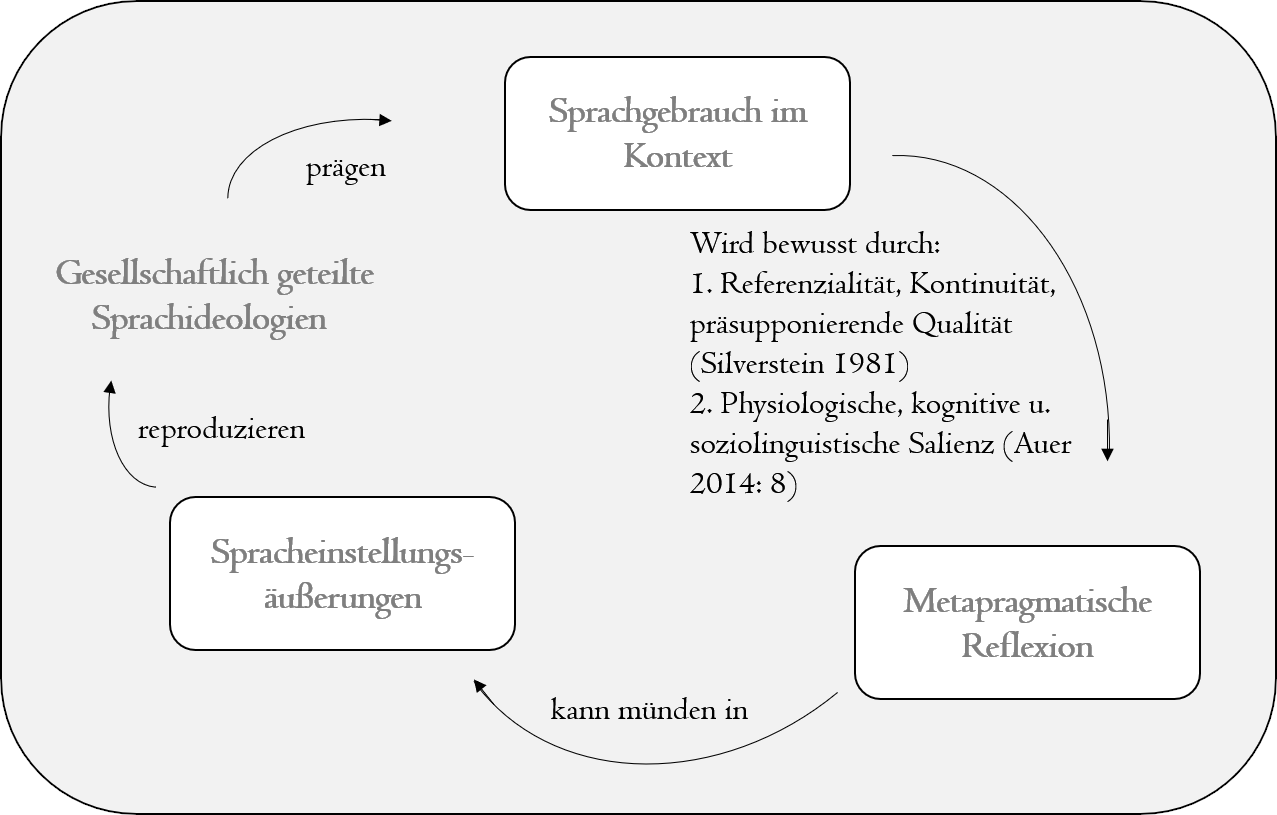
\includegraphics[width=\textwidth]{ModellMetapragmatikundSprachgebrauch}
\caption{Schematische Darstellung des Zusammenhangs von Sprachgebrauch und Metapragmatik}
\label{pic:MetapragmatikundSprachwandel}
\end{figure}
%Schaubild
Dargestellt ist, wie Sprachgebrauch, metapragmatische Bewusstheit, die Reflexion über den wahrgenommenen Sprachgebrauch und die Bewertung des Sprachgebrauchs interagieren. 
Über bestimmte sprachliche Formen reflektieren Sprachbenutzer:innen bewusst. 
Welche das sind, hängt von mehreren Faktoren ab: Einerseits nennt \citet[]{Auer2014} die Salienz, für die Eigenschaften wie etwa Phonemstatus, Frequenz und geografische Reichweite relevant sind, andererseits nennt \citet[]{Silverstein.1981} die Faktoren Referentialität, Kontinuität und präsupponierende Qualität (s. \autoref{sec:MetapragmatischeBewusstheit}). 
Die von diesen Faktoren begünstigte Auffälligkeit ist die Voraussetzung dafür, dass über ein sprachliches Zeichen bewusst reflektiert wird \citep[s.][374]{Butterworth.2011}. 
Ob etwas als auffällig wahrgenommen wird, wird immer vor dem konkreten Kontext entschieden, in dem ein sprachliches Zeichen erscheint. 
Wie dieser Kontext aufgefasst und interpretiert wird, ist wiederum mitbestimmt von sprachideologischen Vorstellungen.
Gesellschaftlich geteilte Sprachideologien bilden also gewissermaßen den Hintergrund, vor dem uns sprachliche Zeichen bewusst werden, sodass wir über sie reflektieren.
Damit sind die in einer Gesellschaft bekannten Sprachideologien und persönliche Einstellungen der Sprachbenutzer:innen zu bestimmten Formen, das Wissen über Sprache also, entscheidend dafür, welche sprachlichen Formen bewusst wahrgenommen werden. 
Die bewusste Wahrnehmung kann zu einer Reflexion führen, die ihrerseits Einstellungen und Ideologien hervorbringt, indem sie die bereits vorhandenen bestätigt, hinterfragt oder ergänzt.
Dabei sind persönliche Einstellungen wie Normbewusstheit und -toleranz entscheidend \citep[s.][375]{Butterworth.2011}. 
Die durch den Reflexions- und Bewertungsprozess generierten Sprachurteile \glqq steuern die situative Auswahl zwischen verschiedenen verfügbaren sprachlichen Varianten und wirken sich damit auf die Art des Sprachgebrauchs einer Gesellschaft aus\grqq{} \citep[372]{Butterworth.2011}.
Dieser Sprachgebrauch kann Ausgangspunkt für erneute metapragmatische Reflexion sein, evtl. mit anderen Bewertungsergebnissen, die ihrerseits wieder den Sprachgebrauch prägen. 
Somit formt Metapragmatik sprachliche Variation und damit auch sprachlichen Wandel zu einem erheblichen Maße mit. 
